\chapter{Democritus Junior to the Reader}
\index{Democritus}
\lettrine[lines=4,findent=5pt,nindent=0pt]{G}{entle reader}, I presume thou
wilt be very inquisitive to know what antic or personate actor this is, that so
insolently intrudes upon this common theatre, to the world's view, arrogating
another man's name; whence he is, why he doth it, and what he hath to say;
although, as \authorfootnote{7}he said, \lit{Primum si noluero, non respondebo,
quis coacturus est?}{I am a free man born, and may choose whether I will tell;
who can compel me?} If I be urged, I will as readily reply as that Egyptian in
\authorfootnote{8}\idxname{Plutarch}, when a curious fellow would needs know what he had
in his basket, \li{Quum vides velatam, quid inquiris in rem absconditam}? It
was therefore covered, because he should not know what was in it. Seek not
after that which is hid; if the contents please thee, \authorfootnote{9}"and be
for thy use, suppose the Man in the Moon, or whom thou wilt to be the author;"
I would not willingly be known. Yet in some sort to give thee satisfaction,
which is more than I need, I will show a reason, both of this usurped name,
title, and subject. And first of the name of Democritus; lest any man, by
reason of it, should be deceived, expecting a \worddef{satirical verse}{pasquil}, a satire, some
ridiculous treatise (as I myself should have done), some prodigious tenet, or
paradox of the earth's motion, of infinite worlds, \li{in infinito vacuo, ex
fortuita atomorum collisione}, in an infinite waste, so caused by an accidental
collision of motes in the sun, all which Democritus held, Epicurus and their
master Lucippus of old maintained, and are lately revived by Copernicus,
Brunus, and some others. Besides, it hath been always an ordinary custom, as
\authorfootnote{10}Gellius observes, "for later writers and impostors, to
broach many absurd and insolent fictions, under the name of so noble a
philosopher as Democritus, to get themselves credit, and by that means the more
to be respected," as artificers usually do, \li{Novo qui marmori ascribunt
Praxatilem suo}. 'Tis not so with me.

\translatedverse{%
\begin{latin}
\begin{verse}%
Non hic Centaurus, non Gorgonas, Harpyasque\\*
Invenies, hominem pagina nostra sapit.\\!
\end{verse}%
\end{latin}}{%
\begin{verse}%
No Centaurs here, or Gorgons look to find,\\*
My subject is of man and human kind.\\!
\end{verse}}{%
\attrib{\getauthornote{11}}}

Thou thyself art the subject of my discourse.

\translatedverse{%
\begin{latin}
\begin{verse}%
Quicquid agunt homines, votum, timor, ira, voluptas,\\*
Gaudia, discursus, nostri farrago libelli.\\!
\end{verse}%
\end{latin}}{%
\begin{verse}%
Whate'er men do, vows, fears, in ire, in sport,\\*
Joys, wand'rings, are the sum of my report.\\!
\end{verse}}{%
\attrib{\authorfootnote{12}}}

My intent is no otherwise to use his name, than Mercurius Gallobelgicus,
Mercurius Britannicus, use the name of Mercury, \authorfootnote{13}Democritus
Christianus, \etc{}; although there be some other circumstances for which I
have masked myself under this vizard, and some peculiar respect which I cannot
so well express, until I have set down a brief character of this our
Democritus, what he was, with an epitome of his life.

\begin{figure}[H]
  \begingroup
  \centering
  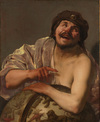
\includegraphics[keepaspectratio,width=0.7\textwidth]{democritus-small.jpg}
  \captionart{Democritus}
  \label{fig:democritus}
\end{figure}

Democritus, as he is described by \authorfootnote{14}Hippocrates and
\authorfootnote{15}Laertius, was a little wearish old man, very melancholy by
nature, averse from company in his latter days, \authorfootnote{16}and much
given to solitariness, a famous philosopher in his age,
\authorfootnote{17}\lit{coaevus}{of the same age} with Socrates, wholly
addicted to his studies at the last, and to a private life: wrote many
excellent works, a great divine, according to the divinity of those times, an
expert physician, a politician, an excellent mathematician, as
\authorfootnote{18}Diacosmus and the rest of his works do witness. He was much
delighted with the studies of husbandry, saith \authorfootnote{19}Columella,
and often I find him cited by \authorfootnote{20}Constantinus and others
treating of that subject. He knew the natures, differences of all beasts,
plants, fishes, birds; and, as some say, could \authorfootnote{21}understand
the tunes and voices of them. In a word, he was \li{omnifariam doctus}, a
general scholar, a great student; and to the intent he might better
contemplate, \authorfootnote{22}I find it related by some, that he put out his
eyes, and was in his old age voluntarily blind, yet saw more than all Greece
besides, and \authorfootnote{23}writ of every subject, \li{Nihil in toto
opificio naturae, de quo non scripsit}. \authorfootnote{24}A man of an
excellent wit, profound conceit; and to attain knowledge the better in his
younger years, he travelled to Egypt and \authorfootnote{25}Athens, to confer
with learned men, \authorfootnote{26}"admired of some, despised of others."
After a wandering life, he settled at Abdera, a town in Thrace, and was sent
for thither to be their lawmaker, recorder, or town-clerk, as some will; or as
others, he was there bred and born. Howsoever it was, there he lived at last in
a garden in the suburbs, wholly betaking himself to his studies and a private
life, \authorfootnote{27}"saving that sometimes he would walk down to the
haven," \authorfootnote{28}"and laugh heartily at such variety of ridiculous
objects, which there he saw." Such a one was Democritus.

But in the mean time, how doth this concern me, or upon what reference do I
usurp his habit? I confess, indeed, that to compare myself unto him for aught I
have yet said, were both impudency and arrogancy. I do not presume to make any
parallel, \lit{Antistat mihi millibus trecentis}{he is immeasurably ahead of
me}, \authorfootnote{29}\lit{parvus sum, nullus sum, altum nec spiro, nec
spero}{I am insignificant, a nobody with little ambition and small prospects}.
Yet thus much I will say of myself, and that I hope without all suspicion of
pride, or self-conceit, I have lived a silent, sedentary, solitary, private
life, \lit{mihi et musis}{for myself and my studies} in the University, as long
almost as Xenocrates in Athens, \lit{ad senectam fere}{practically to old age}
to learn wisdom as he did, penned up most part in my study. For I have been
brought up a student in the most flourishing college of Europe,
\authorfootnote{30}\li{augustissimo collegio}, and can brag with
\authorfootnote{31}Jovius, almost, \lit{in ea luce domicilii Vacicani, totius
orbis celeberrimi, per 37 annos multa opportunaque didici}{for 37 years I have
made good use of my opportunities for study in the world renowned library of
the Vatican}; for thirty years I have continued (having the use of as good
\authorfootnote{32}libraries as ever he had) a scholar, and would be therefore
loath, either by living as a drone, to be an unprofitable or unworthy member of
so learned and noble a society, or to write that which should be any way
dishonourable to such a royal and ample foundation. Something I have done,
though by my profession a divine, yet \li{turbine raptus ingenii}, as
\authorfootnote{33}he said, out of a running wit, an unconstant, unsettled
mind, I had a great desire (not able to attain to a superficial skill in any)
to have some smattering in all, to be \li{aliquis in omnibus, nullus in
singulis}\authorlatintrans{34}, which \authorfootnote{35}Plato commends, out of
him \authorfootnote{36}Lipsius approves and furthers, "as fit to be imprinted
in all curious wits, not to be a slave of one science, or dwell altogether in
one subject, as most do, but to rove abroad, \lit{centum puer artium}{one who
can turn his hand to anything}, to have an oar in every man's boat, to
\authorfootnote{37}taste of every dish, and sip of every cup," which, saith
\authorfootnote{38}Montaigne, was well performed by Aristotle, and his learned
countryman Adrian Turnebus. This roving humour (though not with like success) I
have ever had, and like a ranging spaniel, that barks at every bird he sees,
leaving his game, I have followed all, saving that which I should, and may
justly complain, and truly, \li{qui ubique est, nusquam
est}\authorlatintrans{39}, which \authorfootnote{40}Gesner did in modesty, that
I have read many books, but to little purpose, for want of good method; I have
confusedly tumbled over divers authors in our libraries, with small profit, for
want of art, order, memory, judgment. I never travelled but in map or card, in
which mine unconfined thoughts have freely expatiated, as having ever been
especially delighted with the study of Cosmography. \authorfootnote{41}Saturn
was lord of my geniture, culminating, \etc{}, and Mars principal significator
of manners, in partile conjunction with my ascendant; both fortunate in their
houses, \etc{} I am not poor, I am not rich; \li{nihil est, nihil deest}, I
have little, I want nothing: all my treasure is in Minerva's tower. Greater
preferment as I could never get, so am I not in debt for it, I have a
competence (\lit{laus Deo}{praise God}) from my noble and munificent patrons,
though I live still a collegiate student, as Democritus in his garden, and lead
a monastic life, \lit{ipse mihi theatrum}{sufficient entertainment to myself},
sequestered from those tumults and troubles of the world, \li{Et tanquam in
specula positus}, (\authorfootnote{42}as he said) in some high place above you
all, like Stoicus Sapiens, \lit{omnia saecula, praeterita presentiaque videns,
uno velut intuitu}{the stoic surveying with one sweep all ages down to the
present}, I hear and see what is done abroad, how others
\authorfootnote{43}run, ride, turmoil, and macerate themselves in court and
country, far from those wrangling lawsuits, \li{aulia vanitatem, fori
ambitionem, ridere mecum soleo}: I laugh at all, \authorfootnote{44}only
secure, lest my suit go amiss, my ships perish, corn and cattle miscarry, trade
decay, I have no wife nor children good or bad to provide for. A mere spectator
of other men's fortunes and adventures, and how they act their parts, which
methinks are diversely presented unto me, as from a common theatre or scene. I
hear new news every day, and those ordinary rumours of war, plagues, fires,
inundations, thefts, murders, massacres, meteors, comets, spectrums, prodigies,
apparitions, of towns taken, cities besieged in France, Germany, Turkey,
Persia, Poland, \etc{}, daily musters and preparations, and such like, which
these tempestuous times afford, battles fought, so many men slain, monomachies,
shipwrecks, piracies and sea-fights; peace, leagues, stratagems, and fresh
alarms. A vast confusion of vows, wishes, actions, edicts, petitions, lawsuits,
pleas, laws, proclamations, complaints, grievances are daily brought to our
ears. New books every day, pamphlets, corantoes, stories, whole catalogues of
volumes of all sorts, new paradoxes, opinions, schisms, heresies, controversies
in philosophy, religion, \etc{} Now come tidings of weddings, maskings,
mummeries, entertainments, jubilees, embassies, tilts and tournaments,
trophies, triumphs, revels, sports, plays: then again, as in a new shifted
scene, treasons, cheating tricks, robberies, enormous villainies in all kinds,
funerals, burials, deaths of princes, new discoveries, expeditions, now
comical, then tragical matters. Today we hear of new lords and officers
created, tomorrow of some great men deposed, and then again of fresh honours
conferred; one is let loose, another imprisoned; one purchaseth, another
breaketh: he thrives, his neighbour turns bankrupt; now plenty, then again
dearth and famine; one runs, another rides, wrangles, laughs, weeps, \etc{}
This I daily hear, and such like, both private and public news, amidst the
gallantry and misery of the world; jollity, pride, perplexities and cares,
simplicity and villainy; subtlety, knavery, candour and integrity, mutually
mixed and offering themselves; I rub on \lit{privus privatus}{in complete
privacy}; as I have still lived, so I now continue, \li{statu quo prius}, left
to a solitary life, and mine own domestic discontents: saving that sometimes,
\lit{ne quid mentiar}{not to conceal anything}, as Diogenes went into the city,
and Democritus to the haven to see fashions, I did for my recreation now and
then walk abroad, look into the world, and could not choose but make some
little observation, \li{non tam sagax observator ac simplex
recitator}\authorlatintrans{45}, not as they did, to scoff or laugh at all, but
with a mixed passion.

\translatedverse{%
\begin{latin}
\begin{verse}%
Bilem s\ae{}pe, jocum vestri movere tumultus.\\!
\end{verse}%
\end{latin}}{%
\begin{verse}%
Ye wretched mimics, whose fond heats have been,\\*
How oft! the objects of my mirth and spleen.
\end{verse}}{%
\attrib{\getauthornote{46}}}

I did sometime laugh and scoff with Lucian, and satirically tax with Menippus,
lament with Heraclitus, sometimes again I was \li{petulanti splene
chachinno}\authorlatintrans{47.5}\authorfootnote{47}, and then again, \li{urere
bilis jecur}\authorfootnote{48}, I was much moved to see that abuse which I
could not mend. In which passion howsoever I may sympathise with him or them,
'tis for no such respect I shroud myself under his name; but either in an
unknown habit to assume a little more liberty and freedom of speech, or if you
will needs know, for that reason and only respect which Hippocrates relates at
large in his Epistle to Damegetus, wherein he doth express, how coming to visit
him one day, he found Democritus in his garden at Abdera, in the suburbs,
\authorfootnote{49}under a shady bower, \authorfootnote{50}with a book on his
knees, busy at his study, sometimes writing, sometimes walking. The subject of
his book was melancholy and madness; about him lay the carcases of many several
beasts, newly by him cut up and anatomised; not that he did contemn God's
creatures, as he told Hippocrates, but to find out the seat of this \li{atra
bilis}, or melancholy, whence it proceeds, and how it was engendered in men's
bodies, to the intent he might better cure it in himself, and by his writings
and observation \authorfootnote{51}teach others how to prevent and avoid it.
Which good intent of his, Hippocrates highly commended: Democritus Junior is
therefore bold to imitate, and because he left it imperfect, and it is now
lost, \li{quasi succenturiator Democriti}, to revive again, prosecute, and
finish in this treatise.

You have had a reason of the name. If the title and inscription offend your
gravity, were it a sufficient justification to accuse others, I could produce
many sober treatises, even sermons themselves, which in their fronts carry more
fantastical names. Howsoever, it is a kind of policy in these days, to prefix a
fantastical title to a book which is to be sold; for, as larks come down to a
day-net, many vain readers will \worddef{delay}{tarry} and stand gazing like
silly passengers at an antic picture in a painter's shop, that will not look at
a judicious piece. And, indeed, as \authorfootnote{52}Scaliger observes,
"nothing more invites a reader than an argument unlooked for, unthought of, and
sells better than a \worddef{vulgar, obscene}{scurrile} pamphlet," \li{tum
maxime cum novitas excitat \authorfootnote{53}palatum}. "Many men," saith
Gellius, "are very conceited in their inscriptions," "and able" (as
\authorfootnote{54}Pliny quotes out of Seneca) "to make him loiter by the way
that went in haste to fetch a midwife for his daughter, now ready to lie down."
For my part, I have honourable \authorfootnote{55}precedents for this which I
have done: I will cite one for all, Anthony Zara, Pap. Epis., his Anatomy of
Wit, in four sections, members, subsections, \etc{}, to be read in our
libraries.

If any man except against the matter or manner of treating of this my subject,
and will demand a reason of it, I can allege more than one; I write of
melancholy, by being busy to avoid
melancholy.\phantomsection\label{mention:being-busy} There is no greater cause
of melancholy than idleness, "no better cure than business," as
\authorfootnote{56}Rhasis holds: and howbeit, \li{stultus labor est
ineptiarum}, to be busy in toys is to small purpose, yet hear that divine
Seneca, \li{aliud agere quam nihil}, better do to no end, than nothing. I wrote
therefore, and busied myself in this playing labour, \lit{oliosaque diligentia
ut vitarem torporum feriandi}{to escape the ennui of idleness by a leisurely
kind of employment} with Vectius in Macrobius, \lit{atque otium in utile
verterem negatium}{and so turn leisure to good account}.

\translatedverse{%
\begin{latin}
\begin{verse}%
Simul et jucunda et idonea dicere vita,\\*
Lectorem delectando simul atque monendo.\\!
\end{verse}%
\end{latin}}{%
\begin{verse}%
Poets would profit or delight mankind,\\*
And with the pleasing have th' instructive joined.\\*
Profit and pleasure, then, to mix with art,\\*
T' inform the judgment, nor offend the heart,\\*
Shall gain all votes.\\!
\end{verse}}{%
\attrib{\getauthornote{57}}}

To this end I write, like them, saith Lucian, that "recite to trees, and
declaim to pillars for want of auditors:" as \authorfootnote{58}Paulus Aegineta
ingenuously confesseth, "not that anything was unknown or omitted, but to
exercise myself," which course if some took, I think it would be good for their
bodies, and much better for their souls; or peradventure as others do, for
fame, to show myself (\li{Scire tuum nihil est, nisi te scire hoc sciat
alter}). I might be of Thucydides' opinion, \authorfootnote{59}"to know a thing
and not to express it, is all one as if he knew it not." When I first took this
task in hand, \li{et quod ait \authorfootnote{60}ille, impellents genio
negotium suscepi}, this I aimed at; \authorfootnote{61}\li{vel ut lenirem
animum scribendo}, to ease my mind by writing; for I had \li{gravidum cor,
foetum caput}, a kind of imposthume in my head, which I was very desirous to be
unladen of, and could imagine no fitter evacuation than this. Besides, I might
not well refrain, for \li{ubi dolor, ibi digitus}, one must needs scratch where
it itches. I was not a little offended with this malady, shall I say my
mistress Melancholy, my Aegeria, or my \li{malus genius}? and for that cause,
as he that is stung with a scorpion, I would expel \li{clavum clavo},
\authorfootnote{62}comfort one sorrow with another, idleness with idleness,
\li{ut ex vipera Theriacum}, make an antidote out of that which was the prime
cause of my disease. Or as he did, of whom \authorfootnote{63}Felix Plater
speaks, that thought he had some of Aristophanes' frogs in his belly, still
crying \li{Breec, okex, coax, coax, oop, oop}, and for that cause studied
physic seven years, and travelled over most part of Europe to ease himself. To
do myself good I turned over such physicians as our libraries would afford, or
my \authorfootnote{64}private friends impart, and have taken this pains. And
why not? Cardan professeth he wrote his book, \bookcite{\textlatin{De
Consolatione}} after his son's death, to comfort himself; so did Tully write of
the same subject with like intent after his daughter's departure, if it be his
at least, or some impostor's put out in his name, which Lipsius probably
suspects. Concerning myself, I can peradventure affirm with Marius in Sallust,
\authorfootnote{65}"that which others hear or read of, I felt and practised
myself; they get their knowledge by books, I mine by melancholising."
\li{Experto crede Roberto}. Something I can speak out of experience,
\li{aerumnabilis experientia me docuit}; and with her in the poet,
\authorfootnote{66}\li{Haud ignara mali miseris succurrere
disco}\authorlatintrans{66.5}; I would help others out of a fellow-feeling;
and, as that virtuous lady did of old, \authorfootnote{67}"being a leper
herself, bestow all her portion to build an hospital for lepers," I will spend
my time and knowledge, which are my greatest fortunes, for the common good of
all.

Yea, but you will infer that this is \authorfootnote{68}\li{actum agere}, an
unnecessary work, \li{cramben bis coctam apponnere}, the same again and again
in other words. To what purpose? \authorfootnote{69}"Nothing is omitted that
may well be said," so thought Lucian in the like theme. How many excellent
physicians have written just volumes and elaborate tracts of this subject? No
news here; that which I have is stolen, from others,
\authorfootnote{70}\li{Dicitque mihi mea pagina fur es}. If that severe doom of
\authorfootnote{71}Synesius be true, "it is a greater offence to steal dead
men's labours, than their clothes," what shall become of most writers? I hold
up my hand at the bar among others, and am guilty of felony in this kind,
\li{habes confitentem reum}, I am content to be pressed with the rest. 'Tis
most true, \li{tenet insanabile multos scribendi cacoethes}, and
\authorfootnote{72}"there is no end of writing of books," as the wiseman found
of old, in this \authorfootnote{73}scribbling age, especially wherein
\authorfootnote{74}"the number of books is without number," (as a worthy man
saith,) "presses be oppressed," and out of an itching humour that every man
hath to show himself, \authorfootnote{75}desirous of fame and honour
(\li{scribimus indocti doctique} ---) he will write no matter what, and scrape
together it boots not whence. \authorfootnote{76}"Bewitched with this desire of
fame," \li{etiam mediis in morbis}, to the disparagement of their health, and
scarce able to hold a pen, they must say something, \authorfootnote{77}"and get
themselves a name," saith Scaliger, "though it be to the downfall and ruin of
many others." To be counted writers, \li{scriptores ut salutentur}, to be
thought and held polymaths and polyhistors, \li{apud imperitum vulgus ob
ventosae nomen artis}, to get a paper-kingdom: \li{nulla spe quaestus sed ampla
famae}, in this precipitate, ambitious age, \li{nunc ut est saeculum, inter
immaturam eruditionem, ambitiosum et praeceps} ('tis
\authorfootnote{78}Scaliger's censure); and they that are scarce auditors,
\li{vix auditores}, must be masters and teachers, before they be capable and
fit hearers. They will rush into all learning, \li{togatam armatam}, divine,
human authors, rake over all indexes and pamphlets for notes, as our merchants
do strange havens for traffic, write great tomes, \li{Cum non sint re vera
doctiores, sed loquaciores}, whereas they are not thereby better scholars, but
greater praters. They commonly pretend public good, but as
\authorfootnote{79}Gesner observes, 'tis pride and vanity that eggs them on; no
news or aught worthy of note, but the same in other terms. \li{Ne feriarentur
fortasse typographi vel ideo scribendum est aliquid ut se vixisse testentur}.
As apothecaries we make new mixtures everyday, pour out of one vessel into
another; and as those old Romans robbed all the cities of the world, to set out
their bad-sited Rome, we skim off the cream of other men's wits, pick the
choice flowers of their tilled gardens to set out our own sterile plots.
\li{Castrant alios ut libros suos per se graciles alieno adipe suffarciant} (so
\authorfootnote{80}Jovius inveighs.) They lard their lean books with the fat of
others' works. \li{Ineruditi fures}, \etc{} A fault that every writer finds, as
I do now, and yet faulty themselves, \authorfootnote{81}\li{Trium literarum
homines}, all thieves; they pilfer out of old writers to stuff up their new
comments, scrape Ennius' dunghills, and out of \authorfootnote{82}Democritus'
pit, as I have done. By which means it comes to pass, \authorfootnote{83}"that
not only libraries and shops are full of our putrid papers, but every
close-stool and jakes," \li{Scribunt carmina quae legunt cacantes}; they serve
to put under pies, to \authorfootnote{84}lap spice in, and keep roast meat from
burning. "With us in France," saith \authorfootnote{85}Scaliger, "every man
hath liberty to write, but few ability." \authorfootnote{86}"Heretofore
learning was graced by judicious scholars, but now noble sciences are vilified
by base and illiterate scribblers," that either write for vainglory, need, to
get money, or as Parasites to flatter and collogue with some great men, they
put cut \authorfootnote{87}\li{burras, quisquiliasque ineptiasque}.
\authorfootnote{88}Amongst so many thousand authors you shall scarce find one,
by reading of whom you shall be any whit better, but rather much worse,
\li{quibus inficitur potius, quam perficitur}, by which he is rather infected
than any way perfected.

\translatedverse{%
\begin{latin}
\begin{verse}%
------Qui talia legit,\\*
Quid didicit tandem, quid scit nisi somnia, nugas?\\!
\end{verse}%
\end{latin}}{%\authorlatintrans{89.5}
\begin{verse}%
What does any one, who reads such works,\\*
learn or know but dreams and trifling things.\\!
\end{verse}}{%
\attrib{\getauthornote{89}}}

So that oftentimes it falls out (which Callimachus taxed of old) a great book
is a great mischief. \authorfootnote{90}Cardan finds fault with Frenchmen and
Germans, for their scribbling to no purpose, \li{non inquit ab edendo deterreo,
modo novum aliquid inveniant}, he doth not bar them to write, so that it be
some new invention of their own; but we weave the same web still, twist the
same rope again and again; or if it be a new invention, 'tis but some bauble or
toy which idle fellows write, for as idle fellows to read, and who so cannot
invent? \authorfootnote{91}"He must have a barren wit, that in this scribbling
age can forge nothing. \authorfootnote{92}Princes show their armies, rich men
vaunt their buildings, soldiers their manhood, and scholars vent their toys;"
they must read, they must hear whether they will or no.

\translatedverse{%
\begin{latin}
\begin{verse}%
Et quodcunque semel chartis illeverit, omnes\\*
Gestiet a furno redeuntes scire lacuque,\\*
Et pueros et anus------\\!
\end{verse}%
\end{latin}}{%
\begin{verse}%
What once is said and writ, all men must know,\\*
Old wives and children as they come and go.\\!
\end{verse}}{%
\attrib{\getauthornote{93}}}


"What a company of poets hath this year brought out," as Pliny complains to
Sossius Sinesius. \authorfootnote{94}"This April every day some or other have
recited." What a catalogue of new books all this year, all this age (I say),
have our Frankfort Marts, our domestic Marts brought out? Twice a year,
\authorfootnote{95}\li{Proferunt se nova ingenia et ostentant}, we stretch our
wits out, and set them to sale, \li{magno conatu nihil agimus}. So that which
\authorfootnote{96}Gesner much desires, if a speedy reformation be not had, by
some prince's edicts and grave supervisors, to restrain this liberty, it will
run on \li{in infinitum}. \li{Quis tam avidus librorum helluo}, who can read
them? As already, we shall have a vast chaos and confusion of books, we are
\authorfootnote{97}oppressed with them, \authorfootnote{98}our eyes ache with
reading, our fingers with turning. For my part I am one of the number, \li{nos
numerus sumus}, (we are mere ciphers): I do not deny it, I have only this of
Macrobius to say for myself, \li{Omne meum, nihil meum}, 'tis all mine, and
none mine. As a good housewife out of divers fleeces weaves one piece of cloth,
a bee gathers wax and honey out of many flowers, and makes a new bundle of all,
\li{Floriferis ut apes in saltibus omnia libant}, I have laboriously
\authorfootnote{99}collected this cento out of divers writers, and that
\li{sine injuria}, I have wronged no authors, but given every man his own;
which \authorfootnote{100}Hierom so much commends in Nepotian; he stole not
whole verses, pages, tracts, as some do nowadays, concealing their authors'
names, but still said this was Cyprian's, that Lactantius, that Hilarius, so
said Minutius Felix, so Victorinus, thus far Arnobius: I cite and quote mine
authors (which, howsoever some illiterate scribblers account pedantical, as a
cloak of ignorance, and opposite to their affected fine style, I must and will
use) \li{sumpsi, non suripui}; and what Varro, \bookcite{\textlatin{lib. 6. de
re rust.}} speaks of bees, \li{minime maleficae nullius opus vellicantes
faciunt delerius}, I can say of myself, Whom have I injured? The matter is
theirs most part, and yet mine, \li{apparet unde sumptum sit} (which Seneca
approves), \li{aliud tamen quam unde sumptum sit apparet}, which nature doth
with the aliment of our bodies incorporate, digest, assimilate, I do
\li{concoquere quod hausi}, dispose of what I take. I make them pay tribute, to
set out this my Maceronicon, the method only is mine own, I must usurp that of
\authorfootnote{101}Wecker \li{e Ter. nihil dictum quod non dictum prius,
methodus sola artificem ostendit}, we can say nothing but what hath been said,
the composition and method is ours only, and shows a scholar. Oribasius,
Aesius, Avicenna, have all out of Galen, but to their own method, \li{diverso
stilo, non diversa fide}. Our poets steal from Homer; he spews, saith Aelian,
they lick it up. Divines use Austin's words verbatim still, and our
story-dressers do as much; he that comes last is commonly best,

\translatedverse{%
\begin{latin}
\begin{verse}%
------donec quid grandius aetas\\*
Postera sorsque ferat melior.------\\!
\end{verse}%
\end{latin}}{%\setauthornote{102}
\begin{verse}%
until a later age and a happier lot\\*
produce something more truly grand.\\!
\end{verse}}{}

Though there were many giants of old in physic and philosophy, yet I say with
\authorfootnote{103}Didacus Stella, "A dwarf standing on the shoulders of a
giant may see farther than a giant himself;" I may likely add, alter, and see
farther than my predecessors; and it is no greater prejudice for me to indite
after others, than for Aelianus Montaltus, that famous physician, to write
\bookcite{\textlatin{de morbis capitis}} after Jason Pratensis, Heurnius,
Hildesheim, \etc{}, many horses to run in a race, one logician, one
rhetorician, after another. Oppose then what thou wilt,

\begin{latin}
\begin{verse}%
Allatres licet usque nos et usque\\*
Et gannitibus improbis lacessas.\\!
\end{verse}%
\end{latin}


I solve it thus. And for those other faults of barbarism,
\authorfootnote{104}Doric dialect, extemporanean style, tautologies, apish
imitation, a rhapsody of rags gathered together from several dunghills,
excrements of authors, toys and fopperies confusedly tumbled out, without art,
invention, judgment, wit, learning, harsh, raw, rude, fantastical, absurd,
insolent, indiscreet, ill-composed, indigested, vain, scurrile, idle, dull, and
dry; I confess all ('tis partly affected), thou canst not think worse of me
than I do of myself. 'Tis not worth the reading, I yield it, I desire thee not
to lose time in perusing so vain a subject, I should be peradventure loath
myself to read him or thee so writing; 'tis not \li{operae, pretium}. All I say
is this, that I have \authorfootnote{105}precedents for it, which Isocrates
calls \li{perfugium iis qui peccant}, others as absurd, vain, idle, illiterate,
\etc{} \li{Nonnulli alii idem fecerunt}; others have done as much, it may be
more, and perhaps thou thyself, \li{Novimus et qui te}, \etc{} We have all our
faults; \li{scimus, et hanc, veniaim}, \etc{}; \authorfootnote{106}thou
censurest me, so have I done others, and may do thee, \li{Cedimus inque vicem},
\etc{}, 'tis \li{lex talionis, quid pro quo}.

Go now, censure, criticise, scoff, and rail.

\translatedverse{%
\begin{latin}
\begin{verse}%
Nasutus cis usque licet, sis denique nasus:\\*
Non potes in nugas dicere plura meas,\\*
Ipse ego quam dixi, \etc{}\\!
\end{verse}%
\end{latin}}{%
\begin{verse}%
Wert thou all scoffs and flouts, a very Momus,\\*
Than we ourselves, thou canst not say worse of us.\\!
\end{verse}}{%
\attrib{\getauthornote{107}}}

Thus, as when women scold, have I cried whore first, and in some men's censures
I am afraid I have overshot myself, \li{Laudare se vani, vituperare stulti}, as
I do not arrogate, I will not derogate. \li{Primus vestrum non sum, nec imus},
I am none of the best, I am none of the meanest of you. As I am an inch, or so
many feet, so many parasangs, after him or him, I may be peradventure an ace
before thee. Be it therefore as it is, well or ill, I have essayed, put myself
upon the stage; I must abide the censure, I may not escape it. It is most true,
\li{stylus virum arguit}, our style bewrays us, and as
\authorfootnote{108}hunters find their game by the trace, so is a man's genius
descried by his works, \li{Multo melius ex sermone quam lineamentis, de moribus
hominum judicamus}; it was old Cato's rule. I have laid myself open (I know it)
in this treatise, turned mine inside outward: I shall be censured, I doubt not;
for, to say truth with Erasmus, \li{nihil morosius hominum judiciis}, there is
nought so peevish as men's judgments; yet this is some comfort, \li{ut palata,
sic judicia}, our censures are as various as our palates.

\translatedverse{%
\begin{latin}
\begin{verse}%
Tres mihi convivae prope dissentire videntur,\\*
Poscentes vario multum diversa palato, \etc{}\\!
\end{verse}%
\end{latin}}{%
\begin{verse}%
Three guests I have, dissenting at my feast,\\*
Requiring each to gratify his taste\\*
With different food.\\!
\end{verse}}{%
\attrib{\getauthornote{109}}}

Our writings are as so many dishes, our readers guests, our books like beauty,
that which one admires another rejects; so are we approved as men's fancies are
inclined. \li{Pro captu lectoris habent sua fata libelli}. That which is most
pleasing to one is \li{amaracum sui}, most harsh to another. \li{Quot homines,
tot sententiae}, so many men, so many minds: that which thou condemnest he
commends. \authorfootnote{110}\li{Quod petis, id sane est invisum acidumque
duobus}. He respects matter, thou art wholly for words; he loves a loose and
free style, thou art all for neat composition, strong lines, hyperboles,
allegories; he desires a fine frontispiece, enticing pictures, such as
\authorfootnote{111}Hieron. Natali the Jesuit hath cut to the Dominicals, to
draw on the reader's attention, which thou rejectest; that which one admires,
another explodes as most absurd and ridiculous. If it be not point blank to his
humour, his method, his conceit, \authorfootnote{112}\li{si quid, forsan
omissum, quod is animo conceperit, si quae dictio}, \etc{} If aught be omitted,
or added, which he likes, or dislikes, thou art \li{mancipium paucae
lectionis}, an idiot, an ass, \li{nullus es}, or \li{plagiarius}, a trifler, a
trivant, thou art an idle fellow; or else it is a thing of mere industry, a
collection without wit or invention, a very toy.
\authorfootnote{113}\li{Facilia sic putant omnes quae jam facta, nec de
salebris cogitant, ubi via strata}; so men are valued, their labours vilified
by fellows of no worth themselves, as things of nought, who could not have done
as much. \li{Unusquisque abundat sensu suo}, every man abounds in his own
sense; and whilst each particular party is so affected, how should one please
all?

\translatedverse{%
\begin{latin}
\begin{verse}%
Quid dem? quid non dem? Renuis tu quod jubet ille.\\!
\end{verse}%
\end{latin}}{%
\begin{verse}%
------What courses must I choose?\\*
What not? What both would order you refuse.\\!
\end{verse}}{%
\attrib{\getauthornote{114}}}


How shall I hope to express myself to each man's humour and
\authorfootnote{115}conceit, or to give satisfaction to all? Some understand
too little, some too much, \li{qui similiter in legendos libros, atque in
salutandos homines irruunt, non cogitantes quales, sed quibus vestibus induti
sint}, as \authorfootnote{116}Austin observes, not regarding what, but who
write, \authorfootnote{117}\li{orexin habet auctores celebritas}, not valuing
the metal, but stamp that is upon it, \li{Cantharum aspiciunt, non quid in eo}.
If he be not rich, in great place, polite and brave, a great doctor, or full
fraught with grand titles, though never so well qualified, he is a dunce; but,
as \authorfootnote{118}Baronius hath it of Cardinal Caraffa's works, he is a
mere hog that rejects any man for his poverty. Some are too partial, as friends
to overween, others come with a prejudice to carp, vilify, detract, and scoff;
(\li{qui de me forsan, quicquid est, omni contemptu contemptius judicant}) some
as bees for honey, some as spiders to gather poison. What shall I do in this
case? As a Dutch host, if you come to an inn in. Germany, and dislike your
fare, diet, lodging, \etc{}, replies in a surly tone,
\authorfootnote{119}\li{aliud tibi quaeras diversorium}, if you like not this,
get you to another inn: I resolve, if you like not my writing, go read
something else. I do not much esteem thy censure, take thy course, it is not as
thou wilt, nor as I will, but when we have both done, that of
\authorfootnote{120}Plinius Secundus to Trajan will prove true, "Every man's
witty labour takes not, except the matter, subject, occasion, and some
commending favourite happen to it." If I be taxed, exploded by thee and some
such, I shall haply be approved and commended by others, and so have been
(\li{Expertus loquor}), and may truly say with \authorfootnote{121}Jovius in
like case, \li{(absit verbo jactantia) heroum quorundam, pontificum, et virorum
nobilium familiaritatem et amicitiam, gratasque gratias, et multorum
\authorfootnote{122}bene laudatorum laudes sum inde promeritus}, as I have been
honoured by some worthy men, so have I been vilified by others, and shall be.
At the first publishing of this book, (which \authorfootnote{123}Probus of
Persius satires), \li{editum librum continuo mirari homines, atque avide
deripere caeperunt}, I may in some sort apply to this my work. The first,
second, and third edition were suddenly gone, eagerly read, and, as I have
said, not so much approved by some, as scornfully rejected by others. But it
was Democritus his fortune, \li{Idem admirationi et
\authorfootnote{124}irrisioni habitus}. 'Twas Seneca's fate, that
superintendent of wit, learning, judgment, \authorfootnote{125}\li{ad stuporem
doctus}, the best of Greek and Latin writers, in \idxname{Plutarch}'s opinion;
that "renowned corrector of vice," as, \authorfootnote{126}Fabius terms him,
"and painful omniscious philosopher, that writ so excellently and admirably
well," could not please all parties, or escape censure. How is he vilified by
\authorfootnote{127}Caligula, Agellius, Fabius, and Lipsius himself, his chief
propugner? \li{In eo pleraque pernitiosa}, saith the same Fabius, many childish
tracts and sentences he hath, \li{sermo illaboratus}, too negligent often and
remiss, as Agellius observes, \li{oratio vulgaris et protrita, dicaces et
ineptae, sententiae, eruditio plebeia}, an homely shallow writer as he is.
\li{In partibus spinas et fastidia habet}, saith \authorfootnote{128}Lipsius;
and, as in all his other works, so especially in his epistles, \li{aliae in
argutiis et ineptiis occupantur, intricatus alicubi, et parum compositus, sine
copia rerum hoc fecit}, he jumbles up many things together immethodically,
after the Stoics' fashion, \li{parum ordinavit, multa accumulavit}, \etc{} If
Seneca be thus lashed, and many famous men that I could name, what shall I
expect? How shall I that am \li{vix umbra tanti philosophi} hope to please? "No
man so absolute" (\authorfootnote{129}Erasmus holds) "to satisfy all, except
antiquity, prescription, \etc{}, set a bar." But as I have proved in Seneca,
this will not always take place, how shall I evade? 'Tis the common doom of all
writers, I must (I say) abide it; I seek not applause;
\authorfootnote{130}\li{Non ego ventosa venor suffragia plebis}; again, \li{non
sum adeo informis}, I would not be \authorfootnote{131}vilified:

\begin{latin}
\begin{verse}%
------laudatus abunde,\\*
Non fastiditus si tibi, lector, ero.\\!
\end{verse}%
\end{latin}
\attrib{\getauthornote{132}}

I fear good men's censures, and to their favourable acceptance I submit my labours,

\begin{latin}
\begin{verse}%
------et linguas mancipiorum\\*
Contemno.------\\!
\end{verse}%
\end{latin}
\attrib{\getauthornote{133}}

As the barking of a dog, I securely contemn those malicious and scurrile
obloquies, flouts, calumnies of railers and detractors; I scorn the rest. What
therefore I have said, \li{pro tenuitate mea}, I have said.

One or two things yet I was desirous to have amended if I could, concerning the
manner of handling this my subject, for which I must apologise,
\lit{deprecari}{I pray}, and upon better advice give the friendly reader
notice: it was not mine intent to prostitute my muse in English, or to divulge
\li{secreta Minervae}, but to have exposed this more contract in Latin, if I
could have got it printed. Any scurrile pamphlet is welcome to our mercenary
stationers in English; they print all

\begin{latin}
\begin{verse}%
------cuduntque libellos\\*
In quorum foliis vix simia nuda cacaret;\\!
\end{verse}%
\end{latin}

But in Latin they will not deal; which is one of the reasons
\authorfootnote{134}Nicholas Car, in his oration of the
\worddef{scarcity}{paucity} of English writers, gives, that so many flourishing
wits are smothered in oblivion, lie dead and buried in this our nation. Another
main fault is, that I have not revised the copy, and amended the style, which
now flows \worddef{carelessly}{remissly}, as it was first conceived; but my
leisure would not permit; \li{Feci nec quod potui, nec quod volui}, I confess
it is neither as I would, nor as it should be.

\translatedverse{%
\begin{latin}
\begin{verse}%
Cum relego scripsisse pudet, quia plurima cerno\\*
Me quoque quae fuerant judice digna lini.\\!
\end{verse}%
\end{latin}}{%
\begin{verse}%
When I peruse this tract which I have writ,\\*
I am abash'd, and much I hold unfit.\\!
\end{verse}}{%
\attrib{\getauthornote{135}}}

\li{Et quod gravissimum}, in the matter itself, many things I disallow at this
present, which when I writ, \authorfootnote{136}\li{Non eadem est aetas, non
mens}; I would willingly retract much, \etc{}, but 'tis too late, I can only
crave pardon now for what is amiss.

I might indeed, (had I wisely done) observed that precept of the poet,
\li{------nonumque prematur in annum}, and have taken more care: or, as
Alexander the physician would have done by lapis lazuli, fifty times washed
before it be used, I should have revised, corrected and amended this tract; but
I had not (as I said) that happy leisure, no \worddef{secretary,
scribe}{amanuenses} or assistants. Pancrates in \authorfootnote{137}Lucian,
wanting a servant as he went from Memphis to Coptus in Egypt, took a door bar,
and after some superstitious words pronounced (Eucrates the relator was then
present) made it stand up like a serving-man, fetch him water, turn the spit,
serve in supper, and what work he would besides; and when he had done that
service he desired, turned his man to a stick again. I have no such skill to
make new men at my pleasure, or means to hire them; no whistle to call like the
master of a ship, and bid them run, \etc{} I have no such authority, no such
benefactors, as that noble \authorfootnote{138}Ambrosius was to Origen,
allowing him six or seven amanuenses to write out his dictates; I must for that
cause do my business myself, and was therefore enforced, as a bear doth her
whelps, to bring forth this confused lump; I had not time to lick it into form,
as she doth her young ones, but even so to publish it, as it was first written
\li{quicquid in buccam venit}, in an extemporean style, as
\authorfootnote{139}I do commonly all other exercises, \li{effudi quicquid
dictavit genius meus}, out of a confused company of notes, and writ with as
small deliberation as I do ordinarily speak, without all affectation of big
words, fustian phrases, jingling terms, tropes, strong lines, that like
\authorfootnote{140}Acesta's arrows caught fire as they flew, strains of wit,
brave heats, elegies, hyperbolical exornations, elegancies, \etc{}, which many
so much affect. I am \authorfootnote{141}\li{aquae potor}, drink no wine at
all, which so much improves our modern wits, a loose, plain, rude writer,
\li{ficum, voco ficum et ligonem ligonem} and as free, as loose, \li{idem
calamo quod in mente}, \authorfootnote{142}I call a spade a spade, \li{animis
haec scribo, non auribus}, I respect matter not words; remembering that of
Cardan, \li{verba propter res, non res propter verba}: and seeking with Seneca,
\li{quid scribam, non quemadmodum}, rather \emph{what} than \emph{how} to
write: for as Philo thinks, \authorfootnote{143}"He that is conversant about
matter, neglects words, and those that excel in this art of speaking, have no
profound learning,"

\translatedverse{%
\begin{latin}
\begin{verse}%
Verba nitent phaleris, at nullus verba medullas\\*
Intus habent------\\!
\end{verse}%
\end{latin}}{%
\begin{verse}
Words may be resplendent with ornament,\\*
but they contain no marrow within.\\!
\end{verse}}{%
\attrib{\getauthornote{144}}}

Besides, it was the observation of that wise Seneca, \authorfootnote{145}"when
you see a fellow careful about his words, and neat in his speech, know this for
a certainty, that man's mind is busied about toys, there's no solidity in him."
\li{Non est ornamentum virile concinnitas}: as he said of a nightingale,
\li{------vox es, praeterea nihil}, \etc{} I am therefore in this point a
professed disciple of \authorfootnote{146}Apollonius a scholar of Socrates, I
neglect phrases, and labour wholly to inform my reader's understanding, not to
please his ear; 'tis not my study or intent to compose neatly, which an orator
requires, but to express myself readily and plainly as it happens. So that as a
river runs sometimes precipitate and swift, then dull and slow; now direct,
then \li{per ambages}, now deep, then shallow; now muddy, then clear; now
broad, then narrow; doth my style flow: now serious, then light; now comical,
then satirical; now more elaborate, then remiss, as the present subject
required, or as at that time I was affected. And if thou vouchsafe to read this
treatise, it shall seem no otherwise to thee, than the way to an ordinary
traveller, sometimes fair, sometimes foul; here champaign, there enclosed;
barren, in one place, better soil in another: by woods, groves, hills, dales,
plains, \etc{} I shall lead thee \li{per ardua montium, et lubrica valllum, et
roscida cespitum, et \authorfootnote{147}glebosa camporum}, through variety of
objects, that which thou shalt like and surely dislike.

For the matter itself or method, if it be faulty, consider I pray you that of
\li{Columella, Nihil perfectum, aut a singulari consummatum industria}, no man
can observe all, much is defective no doubt, may be justly taxed, altered, and
avoided in Galen, Aristotle, those great masters. \li{Boni venatoris}
(\authorfootnote{148}one holds) \li{plures feras capere, non omnes}; he is a
good huntsman can catch some, not all: I have done my endeavour. Besides, I
dwell not in this study, \li{Non hic sulcos ducimus, non hoc pulvere
desudamus}, I am but a smatterer, I confess, a stranger,
\authorfootnote{149}here and there I pull a flower; I do easily grant, if a
rigid censurer should criticise on this which I have writ, he should not find
three sole faults, as Scaliger in Terence, but three hundred. So many as he
hath done in Cardan's subtleties, as many notable errors as
\authorfootnote{150}Gul Laurembergius, a late professor of Rostock, discovers
in that anatomy of Laurentius, or Barocius the Venetian in \li{Sacro boscus}.
And although this be a sixth edition, in which I should have been more
accurate, corrected all those former escapes, yet it was \li{magni laboris
opus}, so difficult and tedious, that as carpenters do find out of experience,
'tis much better build a new sometimes, than repair an old house; I could as
soon write as much more, as alter that which is written. If aught therefore be
amiss (as I grant there is), I require a friendly admonition, no bitter
invective, \authorfootnote{151}\li{Sint musis socii Charites, Furia omnis
abesto}, otherwise, as in ordinary controversies, \li{funem contentionis
nectamus, sed cui bono}? We may contend, and likely misuse each other, but to
what purpose? We are both scholars, say,

\translatedverse{%
\begin{latin}
\begin{verse}%
------Arcades ambo\\*
Et Cantare pares, et respondere parati.\\!
\end{verse}%
\end{latin}}{%
\begin{verse}%
Both young Arcadians, both alike inspir'd\\*
To sing and answer as the song requir'd.\\!
\end{verse}}{%
\attrib{\getauthornote{152}}}

If we do wrangle, what shall we get by it? Trouble and wrong ourselves, make
sport to others. If I be convict of an error, I will yield, I will amend.
\li{Si quid bonis moribus, si quid veritati dissentaneum, in sacris vel humanis
literis a me dictum sit, id nec dictum esto}. In the mean time I require a
favourable censure of all faults omitted, harsh compositions, pleonasms of
words, tautological repetitions (though Seneca bear me out, \li{nunquam nimis
dicitur, quod nunquam satis dicitur}) perturbations of tenses, numbers,
printers' faults, \etc{} My translations are sometimes rather paraphrases than
interpretations, \li{non ad verbum}, but as an author, I use more liberty, and
that's only taken which was to my purpose. Quotations are often inserted in the
text, which makes the style more harsh, or in the margin, as it happened. Greek
authors, Plato, \idxname{Plutarch}, Athenaeus, \etc{}, I have cited out of
their interpreters, because the original was not so ready. I have mingled
\li{sacra prophanis}, but I hope not profaned, and in repetition of authors'
names, ranked them \li{per accidens}, not according to chronology; sometimes
neoterics before ancients, as my memory suggested. Some things are here
altered, expunged in this sixth edition, others amended, much added, because
many good \authorfootnote{153}authors in all kinds are come to my hands since,
and 'tis no prejudice, no such indecorum, or oversight.

\translatedverse{%
\begin{latin}
\begin{verse}%
Nunquam ita quicquam bene subducta ratione ad vitam fuit,\\*
Quin res, aetas, usus, semper aliquid apportent novi,\\*
Aliquid moneant, ut illa quae scire te credas, nescias,\\*
Et quae tibi putaris prima, in exercendo ut repudias.\\!
\end{verse}%
\end{latin}}{%
\begin{verse}%
Ne'er was ought yet at first contriv'd so fit,\\*
But use, age, or something would alter it;\\*
Advise thee better, and, upon peruse,\\*
Make thee not say, and what thou tak'st refuse.\\!
\end{verse}}{%
\attrib{\getauthornote{154}}}

But I am now resolved never to put this treatise out again, \li{Ne quid nimis},
I will not hereafter add, alter, or retract; I have done. The last and greatest
exception is, that I, being a divine, have meddled with physic,

\begin{latin}
\begin{verse}%
Tantumne est ab re tua otii tibi,\\*
Aliena ut cures, eaque nihil quae ad te attinent.\\!
\end{verse}%
\end{latin}
\attrib{\getauthornote{155}}%

Which Menedemus objected to Chremes; have I so much leisure, or little business
of mine own, as to look after other men's matters which concern me not? What
have I to do with physic? \li{Quod medicorum est promittant medici}. The
\authorfootnote{156}Lacedaemonians were once in counsel about state matters, a
debauched fellow spake excellent well, and to the purpose, his speech was
generally approved: a grave senator steps up, and by all means would have it
repealed, though good, because \li{dehonestabatur pessimo auctore}, it had no
better an author; let some good man relate the same, and then it should pass.
This counsel was embraced, \li{factum est}, and it was registered forthwith,
\li{Et sic bona sententia mansit, malus auctor mutatus est}. Thou sayest as
much of me, stomachosus as thou art, and grantest, peradventure, this which I
have written in physic, not to be amiss, had another done it, a professed
physician, or so, but why should I meddle with this tract? Hear me speak. There
be many other subjects, I do easily grant, both in humanity and divinity, fit
to be treated of, of which had I written \li{ad ostentationem} only, to show
myself, I should have rather chosen, and in which I have been more conversant,
I could have more willingly luxuriated, and better satisfied myself and others;
but that at this time I was fatally driven upon this rock of melancholy, and
carried away by this by-stream, which, as a rillet, is deducted from the main
channel of my studies, in which I have pleased and busied myself at idle hours,
as a subject most necessary and commodious. Not that I prefer it before
divinity, which I do acknowledge to be the queen of professions, and to which
all the rest are as handmaids, but that in divinity I saw no such great need.
For had I written positively, there be so many books in that kind, so many
commentators, treatises, pamphlets, expositions, sermons, that whole teams of
oxen cannot draw them; and had I been as forward and ambitious as some others,
I might have haply printed a sermon at Paul's Cross, a sermon in St. Marie's
Oxon, a sermon in Christ Church, or a sermon before the right honourable, right
reverend, a sermon before the right worshipful, a sermon in Latin, in English,
a sermon with a name, a sermon without, a sermon, a sermon, \etc{} But I have
been ever as desirous to suppress my labours in this kind, as others have been
to press and publish theirs. To have written in controversy had been to cut off
an hydra's head, \authorfootnote{157}\li{Lis litem generat}, one begets
another, so many duplications, triplications, and swarms of questions. \li{In
sacro bello hoc quod stili mucrone agitur}, that having once begun, I should
never make an end. One had much better, as \authorfootnote{158}Alexander, the
sixth pope, long since observed, provoke a great prince than a begging friar, a
Jesuit, or a seminary priest, I will add, for \li{inexpugnabile genus hoc
hominum}, they are an irrefragable society, they must and will have the last
word; and that with such eagerness, impudence, abominable lying, falsifying,
and bitterness in their questions they proceed, that as he
\authorfootnote{159}said, \li{furorne caecus, an rapit vis acrior, an culpa,
responsum date}? Blind fury, or error, or rashness, or what it is that eggs
them, I know not, I am sure many times, which \authorfootnote{160}Austin
perceived long since, \li{tempestate contentionis, serenitas charitatis
obnubilatur}, with this tempest of contention, the serenity of charity is
overclouded, and there be too many spirits conjured up already in this kind in
all sciences, and more than we can tell how to lay, which do so furiously rage,
and keep such a racket, that as \authorfootnote{161}Fabius said, "It had been
much better for some of them to have been born dumb, and altogether illiterate,
than so far to dote to their own destruction."

\translatedverse{%
\begin{latin}
\begin{verse}%
At melius fuerat non scribere, namque tacere\\*
Tutum semper erit,------\\!
\end{verse}%
\end{latin}}{%\setauthornote{162}
\begin{verse}%
But it would be better not to write,\\*
for silence is the safer course.\\!
\end{verse}}{}

'Tis a general fault, so Severinus the Dane complains \authorfootnote{163}in
physic, "unhappy men as we are, we spend our days in unprofitable questions and
disputations," intricate subtleties, \li{de lana caprina} about moonshine in
the water, "leaving in the mean time those chiefest treasures of nature
untouched, wherein the best medicines for all manner of diseases are to be
found, and do not only neglect them ourselves, but hinder, condemn, forbid, and
scoff at others, that are willing to inquire after them." These motives at this
present have induced me to make choice of this medicinal subject.

If any physician in the mean time shall infer, \li{Ne sutor ultra crepidam},
and find himself grieved that I have intruded into his profession, I will tell
him in brief, I do not otherwise by them, than they do by us. If it be for
their advantage, I know many of their sect which have taken orders, in hope of
a benefice, 'tis a common transition, and why may not a melancholy divine, that
can get nothing but by simony, profess physic? Drusianus an Italian (Crusianus,
but corruptly, Trithemius calls him) \authorfootnote{164}"because he was not
fortunate in his practice, forsook his profession, and writ afterwards in
divinity." Marcilius Ficinus was \li{semel et simul}; a priest and a physician
at once, and \authorfootnote{165}T. Linacer in his old age took orders. The
Jesuits profess both at this time, divers of them \li{permissu superiorum},
\worddef{surgeons}{chirurgeons}, panders, bawds, and midwives, \etc{} Many poor
country-vicars, for want of other means, are driven to their shifts; to turn
mountebanks, quacksalvers, empirics, and if our greedy patrons hold us to such
hard conditions, as commonly they do, they will make most of us work at some
trade, as Paul did, at last turn taskers, maltsters, costermongers, graziers,
sell ale as some have done, or worse. Howsoever in undertaking this task, I
hope I shall commit no great error or \li{indecorum}, if all be considered
aright, I can vindicate myself with Georgius Braunus, and Hieronymus Hemingius,
those two learned divines; who (to borrow a line or two of mine
\authorfootnote{166}elder brother) drawn by a "natural love, the one of
pictures and maps, prospectives and chorographical delights, writ that ample
theatre of cities; the other to the study of genealogies, penned \li{theatrum
genealogicum}." Or else I can excuse my studies with
\authorfootnote{167}Lessius the Jesuit in like case. It is a disease of the
soul on which I am to treat, and as much appertaining to a divine as to a
physician, and who knows not what an agreement there is betwixt these two
professions? A good divine either is or ought to be a good physician, a
spiritual physician at least, as our Saviour calls himself, and was indeed,
Mat. iv. 23; Luke, v. 18; Luke, vii. 8. They differ but in object, the one of
the body, the other of the soul, and use divers medicines to cure; one amends
\li{animam per corpus}, the other \li{corpus per animam} as
\authorfootnote{168}our Regius Professor of physic well informed us in a
learned lecture of his not long since. One helps the vices and passions of the
soul, anger, lust, desperation, pride, presumption, \etc{} by applying that
spiritual physic; as the other uses proper remedies in bodily diseases. Now
this being a common infirmity of body and soul, and such a one that hath as
much need of spiritual as a corporal cure, I could not find a fitter task to
busy myself about, a more apposite theme, so necessary, so commodious, and
generally concerning all sorts of men, that should so equally participate of
both, and require a whole physician. A divine in this compound mixed malady can
do little alone, a physician in some kinds of melancholy much less, both make
an absolute cure.

\translatedverse{%
\begin{latin}
\begin{verse}%
Alterius sic altera poscit opem.\\!
\end{verse}%
\end{latin}}{%
\begin{verse}%
------when in friendship joined\\*
A mutual succour in each other find.\\!
\end{verse}}{%
\attrib{\getauthornote{169}}}

And 'tis proper to them both, and I hope not unbeseeming me, who am by my
profession a divine, and by mine inclination a physician. I had Jupiter in my
sixth house; I say with \authorfootnote{170}Beroaldus, \li{non sum medicus, nec
medicinae prorsus expers}, in the theory of physic I have taken some pains, not
with an intent to practice, but to satisfy myself, which was a cause likewise
of the first undertaking of this subject.

If these reasons do not satisfy thee, good reader, as Alexander Munificus that
bountiful prelate, sometimes bishop of Lincoln, when he had built six castles,
\li{ad invidiam operis eluendam}, saith \authorfootnote{171}Mr. Camden, to take
away the envy of his work (which very words Nubrigensis hath of Roger the rich
bishop of Salisbury, who in king Stephen's time built Shirburn castle, and that
of Devises), to divert the scandal or imputation, which might be thence
inferred, built so many religious houses. If this my discourse be
over-medicinal, or savour too much of humanity, I promise thee that I will
hereafter make thee amends in some treatise of divinity. But this I hope shall
suffice, when you have more fully considered of the matter of this my subject,
\li{rem substratam}, melancholy, madness, and of the reasons following, which
were my chief motives: the generality of the disease, the necessity of the
cure, and the commodity or common good that will arise to all men by the
knowledge of it, as shall at large appear in the ensuing preface. And I doubt
not but that in the end you will say with me, that to anatomise this humour
aright, through all the members of this our Microcosmus, is as great a task, as
to reconcile those chronological errors in the Assyrian monarchy, find out the
quadrature of a circle, the creeks and sounds of the north-east, or north-west
passages, and all out as good a discovery as that hungry
\authorfootnote{172}Spaniard's of \lit{Terra Australis Incognita}{the Unknown
Land of Australia}, as great trouble as to perfect the motion of Mars and
Mercury, which so crucifies our astronomers, or to rectify the Gregorian
Calendar. I am so affected for my part, and hope as
\authorfootnote{173}Theophrastus did by his characters, "That our posterity, O
friend Policles, shall be the better for this which we have written, by
correcting and rectifying what is amiss in themselves by our examples, and
applying our precepts and cautions to their own use." And as that great captain
Zisca would have a drum made of his skin when he was dead, because he thought
the very noise of it would put his enemies to flight, I doubt not but that
these following lines, when they shall be recited, or hereafter read, will
drive away melancholy (though I be gone) as much as Zisca's drum could terrify
his foes. Yet one caution let me give by the way to my present, or my future
reader, who is actually melancholy, that he read not the
\authorfootnote{174}symptoms or prognostics in this following tract, lest by
applying that which he reads to himself, aggravating, appropriating things
generally spoken, to his own person (as melancholy men for the most part do) he
trouble or hurt himself, and get in conclusion more harm than good. I advise
them therefore warily to peruse that tract, \li{Lapides loquitur} (so said
\authorfootnote{175}Agrippa \bookcite{\textlatin{de occ. Phil.}}) \li{et
caveant lectores ne cerebrum iis excutiat}. The rest I doubt not they may
securely read, and to their benefit. But I am over-tedious, I proceed.

Of the necessity and generality of this which I have said, if any man doubt, I
shall desire him to make a brief survey of the world, as
\authorfootnote{176}Cyprian adviseth Donat, "supposing himself to be
transported to the top of some high mountain, and thence to behold the tumults
and chances of this wavering world, he cannot choose but either laugh at, or
pity it." S. Hierom out of a strong imagination, being in the wilderness,
conceived with himself, that he then saw them dancing in Rome; and if thou
shalt either conceive, or climb to see, thou shalt soon perceive that all the
world is mad, that it is melancholy, dotes; that it is (which Epichthonius
Cosmopolites expressed not many years since in a map) made like a fool's head
(with that motto, \li{Caput helleboro dignum}) a crazed head, \li{cavea
stultorum}, a fool's paradise, or as Apollonius, a common prison of gulls,
cheaters, flatterers, \etc{} and needs to be reformed. Strabo in the ninth book
of his geography, compares Greece to the picture of a man, which comparison of
his, Nic. Gerbelius in his exposition of Sophianus' map, approves; the breast
lies open from those Acroceraunian hills in Epirus, to the Sunian promontory in
Attica; Pagae and Magaera are the two shoulders; that Isthmus of Corinth the
neck; and Peloponnesus the head. If this allusion hold, 'tis sure a mad head;
Morea may be Moria; and to speak what I think, the inhabitants of modern Greece
swerve as much from reason and true religion at this day, as that Morea doth
from the picture of a man. Examine the rest in like sort, and you shall find
that kingdoms and provinces are melancholy, cities and families, all creatures,
vegetal, sensible, and rational, that all sorts, sects, ages, conditions, are
out of tune, as in Cebes' table, \li{omnes errorem bibunt}, before they come
into the world, they are intoxicated by error's cup, from the highest to the
lowest have need of physic, and those particular actions in
\authorfootnote{177}Seneca, where father and son prove one another mad, may be
general; Porcius Latro shall plead against us all. For indeed who is not a
fool, melancholy, mad?-- \authorfootnote{178}\li{Qui nil molitur inepte}, who
is not brain-sick? Folly, melancholy, madness, are but one disease, Delirium is
a common name to all. Alexander, Gordonius, Jason Pratensis, Savanarola,
Guianerius, Montaltus, confound them as differing \li{secundum magis et minus};
so doth David, \biblecite{Psal. \rn{xxxvii.} 5}. "I said unto the fools, deal not
so madly," and 'twas an old Stoical paradox, \li{omnes stultos insanire},
\authorfootnote{179}all fools are mad, though some madder than others. And who
is not a fool, who is free from melancholy? Who is not touched more or less in
habit or disposition? If in disposition, "ill dispositions beget habits, if
they persevere," saith \authorfootnote{180}\idxname{Plutarch}, habits either
are, or turn to diseases. 'Tis the same which Tully maintains in the second of
his Tusculans, \li{omnium insipientum animi in morbo sunt, et perturbatorum},
fools are sick, and all that are troubled in mind: for what is sickness, but as
\authorfootnote{181}Gregory Tholosanus defines it, "A dissolution or
perturbation of the bodily league, which health combines:" and who is not sick,
or ill-disposed? in whom doth not passion, anger, envy, discontent, fear and
sorrow reign? Who labours not of this disease? Give me but a little leave, and
you shall see by what testimonies, confessions, arguments, I will evince it,
that most men are mad, that they had as much need to go a pilgrimage to the
Anticyrae (as in \authorfootnote{182}Strabo's time they did) as in our days
they run to Compostella, our Lady of Sichem, or Lauretta, to seek for help;
that it is like to be as prosperous a voyage as that of Guiana, and that there
is much more need of hellebore than of tobacco.

That men are so misaffected, melancholy, mad, giddy-headed, hear the testimony
of Solomon, \biblecite{Eccl. \rn{ii.} 12}. "And I turned to behold wisdom,
madness and folly," \etc{} And \biblecite{ver. 23}: "All his days are sorrow, his
travel grief, and his heart taketh no rest in the night." So that take
melancholy in what sense you will, properly or improperly, in disposition or
habit, for pleasure or for pain, dotage, discontent, fear, sorrow, madness, for
part, or all, truly, or metaphorically, 'tis all one. Laughter itself is
madness according to Solomon, and as St. Paul hath it, "Worldly sorrow brings
death." "The hearts of the sons of men are evil, and madness is in their hearts
while they live," \biblecite{Eccl. \rn{ix.} 3}. "Wise men themselves are no
better." \biblecite{Eccl. \rn{i.} 18}. "In the multitude of wisdom is much grief,
and he that increaseth wisdom, increaseth sorrow," \biblecite{chap. \rn{ii.} 17}.
He hated life itself, nothing pleased him: he hated his labour, all, as
\authorfootnote{183}he concludes, is "sorrow, grief, vanity, vexation of
spirit." And though he were the wisest man in the world, \li{sanctuarium
sapientiae}, and had wisdom in abundance, he will not vindicate himself, or
justify his own actions. "Surely I am more foolish than any man, and have not
the understanding of a man in me," \biblecite{Prov. \rn{xxx.} 2}. Be they
Solomon's words, or the words of Agur, the son of Jakeh, they are canonical.
David, a man after God's own heart, confesseth as much of himself,
\biblecite{Psal. \rn{xxxvii.} 21, 22}. "So foolish was I and ignorant, I was even
as a beast before thee." And condemns all for fools, \biblecite{Psal.
\rn{xciii.}; \rn{xxxii.} 9; \rn{xlix.} 20}. He compares them to "beasts,
horses, and mules, in which there is no understanding." The apostle Paul
accuseth himself in like sort, \biblecite{2 Cor. \rn{ix.} 21}. "I would you would
suffer a little my foolishness, I speak foolishly." "The whole head is sick,"
saith Esay, "and the heart is heavy," \biblecite{cap. \rn{i.} 5}. And makes
lighter of them than of oxen and asses, "the ox knows his owner," \etc{}: read
\biblecite{Deut. \rn{xxxii.} 6}; \biblecite{Jer. \rn{iv.}}; \biblecite{Amos,
\rn{iii.} 1}; \biblecite{Ephes. \rn{v.} 6}. "Be not mad, be not deceived, foolish
Galatians, who hath bewitched you?" How often are they branded with this
epithet of madness and folly? No word so frequent amongst the fathers of the
Church and divines; you may see what an opinion they had of the world, and how
they valued men's actions.

I know that we think far otherwise, and hold them most part wise men that are
in authority, princes, magistrates, \authorfootnote{184}rich men, they are wise
men born, all politicians and statesmen must needs be so, for who dare speak
against them? And on the other, so corrupt is our judgment, we esteem wise and
honest men fools. Which Democritus well signified in an epistle of his to
Hippocrates: \authorfootnote{185}the "Abderites account virtue madness," and so
do most men living. Shall I tell you the reason of it?
\authorfootnote{186}Fortune and Virtue, Wisdom and Folly, their seconds, upon a
time contended in the Olympics; every man thought that Fortune and Folly would
have the worst, and pitied their cases; but it fell out otherwise. Fortune was
blind and cared not where she stroke, nor whom, without laws, \li{Audabatarum
instar}, \etc{} Folly, rash and inconsiderate, esteemed as little what she said
or did. Virtue and Wisdom gave \authorfootnote{187}place, were hissed out, and
exploded by the common people; Folly and Fortune admired, and so are all their
followers ever since: knaves and fools commonly fare and deserve best in
worldlings' eyes and opinions. Many good men have no better fate in their ages:
Achish, \biblecite{1 Sam. \rn{xxi.} 14}, held David for a madman.
\authorfootnote{188}Elisha and the rest were no otherwise esteemed. David was
derided of the common people, \biblecite{Ps. \rn{ix.} 7}, "I am become a monster
to many." And generally we are accounted fools for Christ, \biblecite{1 Cor.
xiv}. "We fools thought his life madness, and his end without honour,"
\biblecite{Wisd. \rn{v.} 4}. Christ and his Apostles were censured in like sort,
\biblecite{John \rn{x.}}; \biblecite{Mark \rn{iii.}}; \biblecite{Acts \rn{xxvi.}} And
so were all Christians in \authorfootnote{189}Pliny's time, \li{fuerunt et
alii, similis dementiae}, \etc{} And called not long after,
\authorfootnote{190}\li{Vesaniae sectatores, eversores hominum, polluti
novatores, fanatici, canes, malefici, venefici, Galilaei homunciones}, \etc{}
'Tis an ordinary thing with us, to account honest, devout, orthodox, divine,
religious, plain-dealing men, idiots, asses, that cannot, or will not lie and
dissemble, shift, flatter, \li{accommodare se ad eum locum ubi nati sunt}, make
good bargains, supplant, thrive, \li{patronis inservire; solennes ascendendi
modos apprehendere, leges, mores, consuetudines recte observare, candide
laudare, fortiter defendere, sententias amplecti, dubitare de nullus, credere
omnia, accipere omnia, nihil reprehendere, caeteraque quae promotionem ferunt
et securitatem, quae sine ambage felicem, reddunt hominem, et vere sapientem
apud nos}; that cannot temporise as other men do, \authorfootnote{191}hand and
take bribes, \etc{} but fear God, and make a conscience of their doings. But
the Holy Ghost that knows better how to judge, he calls them fools. "The fool
hath said in his heart," \biblecite{Psal. \rn{liii.} 1}. "And their ways utter
their folly," \biblecite{Psal. \rn{xlix.} 14}. \authorfootnote{192}"For what can
be more mad, than for a little worldly pleasure to procure unto themselves
eternal punishment?" As Gregory and others inculcate unto us.

Yea even all those great philosophers the world hath ever had in admiration,
whose works we do so much esteem, that gave precepts of wisdom to others,
inventors of Arts and Sciences, Socrates the wisest man of his time by the
Oracle of Apollo, whom his two scholars, \authorfootnote{193}Plato and
\authorfootnote{194}Xenophon, so much extol and magnify with those honourable
titles, "best and wisest of all mortal men, the happiest, and most just;" and
as \authorfootnote{195}Alcibiades incomparably commends him; Achilles was a
worthy man, but Bracides and others were as worthy as himself; Antenor and
Nestor were as good as Pericles, and so of the rest; but none present, before,
or after Socrates, \li{nemo veterum neque eorum qui nunc sunt}, were ever such,
will match, or come near him. Those seven wise men of Greece, those Britain
Druids, Indian Brachmanni, Ethiopian Gymnosophist, Magi of the Persians,
Apollonius, of whom Philostratus, \li{Non doctus, sed natus sapiens}, wise from
his cradle, Eoicuras so much admired by his scholar Lucretius:

\translatedverse{%
\begin{latin}
\begin{verse}%
Qui genus humanum ingenio superavit, et omnes\\*
Perstrinxit stellas exortus ut aetherius sol.\\!
\end{verse}%
\end{latin}}{%
\begin{verse}%
Whose wit excell'd the wits of men as far,\\*
As the sun rising doth obscure a star,\\!
\end{verse}}{}

Or that so much renowned Empedocles,

\begin{latin}
\begin{verse}%
Ut vix humana videatur stirpe creatus.\\!
\end{verse}%
\end{latin}
\attrib{\getauthornote{196}}

All those of whom we read such \authorfootnote{197}hyperbolical eulogiums, as
of Aristotle, that he was wisdom itself in the abstract, \authorfootnote{198}a
miracle of nature, breathing libraries, as Eunapius of Longinus, lights of
nature, giants for wit, quintessence of wit, divine spirits, eagles in the
clouds, fallen from heaven, gods, spirits, lamps of the world, dictators,
\li{Nulla ferant talem saecla futura virum}: monarchs, miracles,
superintendents of wit and learning, \li{oceanus, phoenix, atlas, monstrum,
portentum hominis, orbis universi musaeum, ultimus humana naturae donatus,
naturae maritus},

\begin{latin}
\begin{verse}%
------merito cui doctior orbis\\*
Submissis defert fascibus imperium.\\!
\end{verse}%
\end{latin}

As Aelian writ of Protagoras and Gorgias, we may say of them all, \li{tantum a
sapientibus abfuerunt, quantum a viris pueri}, they were children in respect,
infants, not eagles, but kites; novices, illiterate, \li{Eunuchi sapientiae}.
And although they were the wisest, and most admired in their age, as he
censured Alexander, I do them, there were 10\thinspace{}000 in his army as
worthy captains (had they been in place of command) as valiant as himself;
there were myriads of men wiser in those days, and yet all short of what they
ought to be. \authorfootnote{199}Lactantius, in his book of wisdom, proves them
to be dizzards, fools, asses, madmen, so full of absurd and ridiculous tenets,
and brain-sick positions, that to his thinking never any old woman or sick
person doted worse. \authorfootnote{200}Democritus took all from Leucippus, and
left, saith he, "the inheritance of his folly to Epicurus,"
\authorfootnote{201}\li{insanienti dum sapientiae}, \etc{} The like he holds of
Plato, Aristippus, and the rest, making no difference
\authorfootnote{202}"betwixt them and beasts, saving that they could speak."
\authorfootnote{203}Theodoret in his tract, \bookcite{\textlatin{De cur. grec.
affect.}} manifestly evinces as much of Socrates, whom though that Oracle of
Apollo confirmed to be the wisest man then living, and saved him from plague,
whom 2000 years have admired, of whom some will as soon speak evil as of
Christ, yet \li{re vera}, he was an illiterate idiot, as
\authorfootnote{204}Aristophanes calls him, \li{irriscor et ambitiosus}, as his
master Aristotle terms him, \li{scurra Atticus}, as Zeno, an
\authorfootnote{205}enemy to all arts and sciences, as Athaeneus, to
philosophers and travellers, an opiniative ass, a caviller, a kind of pedant;
for his manners, as Theod. Cyrensis describes him, a
\authorfootnote{206}sodomite, an atheist, (so convict by Anytus) \li{iracundus
et ebrius, dicax}, \etc{} a pot-companion, by \authorfootnote{207}Plato's own
confession, a sturdy drinker; and that of all others he was most sottish, a
very madman in his actions and opinions. Pythagoras was part philosopher, part
magician, or part witch. If you desire to hear more of Apollonius, a great wise
man, sometime paralleled by Julian the apostate to Christ, I refer you to that
learned tract of Eusebius against Hierocles, and for them all to Lucian's
\bookcite{\textlatin{Piscator, Icaromenippus, Necyomantia}}: their actions,
opinions in general were so prodigious, absurd, ridiculous, which they broached
and maintained, their books and elaborate treatises were full of dotage, which
Tully \bookcite{\textlatin{ad Atticum}} long since observed, \li{delirant
plerumque scriptores in libris suis}, their lives being opposite to their
words, they commended poverty to others, and were most covetous themselves,
extolled love and peace, and yet persecuted one another with virulent hate and
malice. They could give precepts for verse and prose, but not a man of them (as
\authorfootnote{208}Seneca tells them home) could moderate his affections.
Their music did show us \li{flebiles modos}, \etc{} how to rise and fall, but
they could not so contain themselves as in adversity not to make a lamentable
tone. They will measure ground by geometry, set down limits, divide and
subdivide, but cannot yet prescribe \li{quantum homini satis}, or keep within
compass of reason and discretion. They can square circles, but understand not
the state of their own souls, describe right lines and crooked, \etc{} but know
not what is right in this life, \li{quid in vita rectum sit, ignorant}; so that
as he said, \li{Nescio an Anticyram ratio illis destinet omnem.} I think all
the Anticyrae will not restore them to their wits, \authorfootnote{209}if these
men now, that held \authorfootnote{210}Xenodotus' heart, Crates' liver,
Epictetus' lantern, were so sottish, and had no more brains than so many
beetles, what shall we think of the commonalty? what of the rest?

Yea, but you will infer, that is true of heathens, if they be conferred with
Christians, \biblecite{1 Cor. \rn{iii.} 19}. "The wisdom of this world is
foolishness with God, earthly and devilish," as James calls it, \biblecite{iii.
15}. "They were vain in their imaginations, and their foolish heart was full of
darkness," \biblecite{Rom. \rn{i.} 21, 22}. "When they professed themselves wise,
became fools." Their witty works are admired here on earth, whilst their souls
are tormented in hell fire. In some sense, \lit{Christiani
Crassiani}{Christians are Crassians}, and if compared
to that wisdom, no better than fools. \li{Quis est sapiens? Solus Deus},
\authorfootnote{211}Pythagoras replies, "God is only wise," \biblecite{Rom.
\rn{xvi.}} Paul determines "only good," as Austin well contends, "and no man
living can be justified in his sight." "God looked down from heaven upon the
children of men, to see if any did understand," \biblecite{Psalm \rn{liii.} 2,
3}, but all are corrupt, err. \biblecite{Rom. \rn{iii.} 12}, "None doeth good,
no, not one." Job aggravates this, \biblecite{iv. 18}, "Behold he found no
steadfastness in his servants, and laid folly upon his angels;" \biblecite{19}.
"How much more on them that dwell in houses of clay?" In this sense we are all
fools, and the \authorfootnote{212}Scripture alone is \li{arx Minervae}, we and
our writings are shallow and imperfect. But I do not so mean; even in our
ordinary dealings we are no better than fools. "All our actions," as
\authorfootnote{213}Pliny told Trajan, "upbraid us of folly," our whole course
of life is but matter of laughter: we are not soberly wise; and the world
itself, which ought at least to be wise by reason of his antiquity, as
\authorfootnote{214}Hugo de Prato Florido will have it, "\li{semper stultizat},
is every day more foolish than other; the more it is whipped, the worse it is,
and as a child will still be crowned with roses and flowers." We are apish in
it, \li{asini bipedes}, and every place is full \li{inversorum Apuleiorum} of
metamorphosed and two-legged asses, \li{inversorum Silenorum}, childish,
\li{pueri instar bimuli, tremula patris dormientis in ulna}. Jovianus Pontanus,
Antonio Dial, brings in some laughing at an old man, that by reason of his age
was a little fond, but as he admonisheth there, \li{Ne mireris mi hospes de hoc
sene}, marvel not at him only, for \li{tota haec civitas delirium}, all our
town dotes in like sort, \authorfootnote{215}we are a company of fools. Ask not
with him in the poet, \authorfootnote{216}\li{Larvae hunc intemperiae
insaniaeque agitant senem}? What madness ghosts this old man, but what madness
ghosts us all? For we are \li{ad unum omnes}, all mad, \li{semel insanivimus
omnes} not once, but alway so, \li{et semel, et simul, et semper}, ever and
altogether as bad as he; and not \li{senex bis puer, delira anus}, but say it
of us all, \li{semper pueri}, young and old, all dote, as Lactantius proves out
of Seneca; and no difference betwixt us and children, saving that, \li{majora
ludimus, et grandioribus pupis}, they play with babies of clouts and such toys,
we sport with greater baubles. We cannot accuse or condemn one another, being
faulty ourselves, \li{deliramenta loqueris}, you talk idly, or as
\authorfootnote{217}Mitio upbraided Demea, \li{insanis, auferte}, for we are as
mad our own selves, and it is hard to say which is the worst. Nay, 'tis
universally so, \li{Vitam regit fortuna, non
sapientia}\authorlatintrans{218.5}.\authorfootnote{218}

When \authorfootnote{219}Socrates had taken great pains to find out a wise man,
and to that purpose had consulted with philosophers, poets, artificers, he
concludes all men were fools; and though it procured him both anger and much
envy, yet in all companies he would openly profess it. When
\authorfootnote{220}Supputius in Pontanus had travelled all over Europe to
confer with a wise man, he returned at last without his errand, and could find
none. \authorfootnote{221}Cardan concurs with him, "Few there are (for aught I
can perceive) well in their wits." So doth \authorfootnote{222}Tully, "I see
everything to be done foolishly and unadvisedly."

\translatedverse{%
\begin{latin}
\begin{verse}%
Ille sinistrorsum, hic dextrorsum, unus utrique\\*
Error, sed variis illudit partibus omnes.\\!
\end{verse}%
\end{latin}}{%
\begin{verse}%
One reels to this, another to that wall,\\*
'Tis the same error that deludes them all.\\!
\end{verse}}{}

\authorfootnote{223}They dote all, but not alike, \textgreek{Μανία γαρ πᾶσιν
ὁμοια}, not in the same kind, "One is covetous, a second lascivious, a third
ambitious, a fourth envious, \etc{}" as Damasippus the Stoic hath well
illustrated in the poet,

\translatedverse{%
\begin{latin}
\begin{verse}%
Desipiunt omnes aeque ac tu.\\!
\end{verse}%
\end{latin}}{%
\begin{verse}%
And they who call you fool, with equal claim\\*
May plead an ample title to the name.\\!
\end{verse}}{%
\attrib{\getauthornote{224}}}

'Tis an inbred malady in every one of us, there is \li{seminarium stultitiae},
a seminary of folly, "which if it be stirred up, or get ahead, will run \li{in
infinitum}, and infinitely varies, as we ourselves are severally addicted,"
saith \authorfootnote{225}Balthazar Castilio: and cannot so easily be rooted
out, it takes such fast hold, as Tully holds, \li{altae radices stultitiae},
\authorfootnote{226}so we are bred, and so we continue. Some say there be two
main defects of wit, error and ignorance, to which all others are reduced; by
ignorance we know not things necessary, by error we know them falsely.
Ignorance is a privation, error a positive act. From ignorance comes vice, from
error heresy, \etc{} But make how many kinds you will, divide and subdivide,
few men are free, or that do not impinge on some one kind or other.
\authorfootnote{227}\li{Sic plerumque agitat stultos inscitia}, as he that
examines his own and other men's actions shall find.

\authorfootnote{228}Charon in Lucian, as he wittily feigns, was conducted by
Mercury to such a place, where he might see all the world at once; after he had
sufficiently viewed, and looked about, Mercury would needs know of him what he
had observed: He told him that he saw a vast multitude and a promiscuous, their
habitations like molehills, the men as emmets, "he could discern cities like so
many hives of bees, wherein every bee had a sting, and they did nought else but
sting one another, some domineering like hornets bigger than the rest, some
like filching wasps, others as drones." Over their heads were hovering a
confused company of perturbations, hope, fear, anger, avarice, ignorance,
\etc{}, and a multitude of diseases hanging, which they still pulled on their
pates. Some were brawling, some fighting, riding, running, \li{sollicite
ambientes, callide litigantes} for toys and trifles, and such momentary things,
Their towns and provinces mere factions, rich against poor, poor against rich,
nobles against artificers, they against nobles, and so the rest. In conclusion,
he condemned them all for madmen, fools, idiots, asses, \li{O stulti, quaenam
haec est amentia}? O fools, O madmen, he exclaims, \li{insana studia, insani
labores}, \etc{} Mad endeavours, mad actions, mad, mad, mad,
\authorfootnote{229}\li{O saeclum insipiens et infacetum}, a giddy-headed age.
Heraclitus the philosopher, out of a serious meditation of men's lives, fell a
weeping, and with continual tears bewailed their misery, madness, and folly.
Democritus on the other side, burst out a laughing, their whole life seemed to
him so ridiculous, and he was so far carried with this ironical passion, that
the citizens of Abdera took him to be mad, and sent therefore ambassadors to
Hippocrates, the physician, that he would exercise his skill upon him. But the
story is set down at large by Hippocrates, in his epistle to Damogetus, which
because it is not impertinent to this discourse, I will insert verbatim almost
as it is delivered by Hippocrates himself, with all the circumstances belonging
unto it.

When Hippocrates was now come to Abdera, the people of the city came flocking
about him, some weeping, some intreating of him, that he would do his best.
After some little repast, he went to see Democritus, the people following him,
whom he found (as before) in his garden in the suburbs all alone,
\authorfootnote{230}"sitting upon a stone under a plane tree, without hose or
shoes, with a book on his knees, cutting up several beasts, and busy at his
study." The multitude stood gazing round about to see the congress.
Hippocrates, after a little pause, saluted him by his name, whom he resaluted,
ashamed almost that he could not call him likewise by his, or that he had
forgot it. Hippocrates demanded of him what he was doing: he told him that he
was \authorfootnote{231}"busy in cutting up several beasts, to find out the
cause of madness and melancholy." Hippocrates commended his work, admiring his
happiness and leisure. And why, quoth Democritus, have not you that leisure?
Because, replied Hippocrates, domestic affairs hinder, necessary to be done for
ourselves, neighbours, friends; expenses, diseases, frailties and mortalities
which happen; wife, children, servants, and such business which deprive us of
our time. At this speech Democritus profusely laughed (his friends and the
people standing by, weeping in the mean time, and lamenting his madness).
Hippocrates asked the reason why he laughed. He told him, at the vanities and
the fopperies of the time, to see men so empty of all virtuous actions, to hunt
so far after gold, having no end of ambition; to take such infinite pains for a
little glory, and to be favoured of men; to make such deep mines into the earth
for gold, and many times to find nothing, with loss of their lives and
fortunes. Some to love dogs, others horses, some to desire to be obeyed in many
provinces, \authorfootnote{232}and yet themselves will know no obedience.
\authorfootnote{233}Some to love their wives dearly at first, and after a while
to forsake and hate them; begetting children, with much care and cost for their
education, yet when they grow to man's estate, \authorfootnote{234}to despise,
neglect, and leave them naked to the world's mercy. \authorfootnote{235}Do not
these behaviours express their intolerable folly? When men live in peace, they
covet war, detesting quietness, \authorfootnote{236}deposing kings, and
advancing others in their stead, murdering some men to beget children of their
wives. How many strange humours are in men! When they are poor and needy, they
seek riches, and when they have them, they do not enjoy them, but hide them
under ground, or else wastefully spend them. O wise Hippocrates, I laugh at
such things being done, but much more when no good comes of them, and when they
are done to so ill purpose. There is no truth or justice found amongst them,
for they daily plead one against another, \authorfootnote{237}the son against
the father and the mother, brother against brother, kindred and friends of the
same quality; and all this for riches, whereof after death they cannot be
possessors. And yet notwithstanding they will defame and kill one another,
commit all unlawful actions, contemning God and men, friends and country. They
make great account of many senseless things, esteeming them as a great part of
their treasure, statues, pictures, and such like movables, dear bought, and so
cunningly wrought, as nothing but speech wanteth in them,
\authorfootnote{238}and yet they hate living persons speaking to them.
\authorfootnote{239}Others affect difficult things; if they dwell on firm land
they will remove to an island, and thence to land again, being no way constant
to their desires. They commend courage and strength in wars, and let themselves
be conquered by lust and avarice; they are, in brief, as disordered in their
minds, as Thersites was in his body. And now, methinks, O most worthy
Hippocrates, you should not reprehend my laughing, perceiving so many fooleries
in men; \authorfootnote{240}for no man will mock his own folly, but that which
he seeth in a second, and so they justly mock one another. The drunkard calls
him a glutton whom he knows to be sober. Many men love the sea, others
husbandry; briefly, they cannot agree in their own trades and professions, much
less in their lives and actions.

When Hippocrates heard these words so readily uttered, without premeditation,
to declare the world's vanity, full of ridiculous contrariety, he made answer,
that necessity compelled men to many such actions, and divers wills ensuing
from divine permission, that we might not be idle, being nothing is so odious
to them as sloth and negligence. Besides, men cannot foresee future events, in
this uncertainty of human affairs; they would not so marry, if they could
foretell the causes of their dislike and separation; or parents, if they knew
the hour of their children's death, so tenderly provide for them; or an
husbandman sow, if he thought there would be no increase; or a merchant
adventure to sea, if he foresaw shipwreck; or be a magistrate, if presently to
be deposed. Alas, worthy Democritus, every man hopes the best, and to that end
he doth it, and therefore no such cause, or ridiculous occasion of laughter.

Democritus hearing this poor excuse, laughed again aloud, perceiving he wholly
mistook him, and did not well understand what he had said concerning
perturbations and tranquillity of the mind. Insomuch, that if men would govern
their actions by discretion and providence, they would not declare themselves
fools as now they do, and he should have no cause of laughter; but (quoth he)
they swell in this life as if they were immortal, and demigods, for want of
understanding. It were enough to make them wise, if they would but consider the
mutability of this world, and how it wheels about, nothing being firm and sure.
He that is now above, tomorrow is beneath; he that sate on this side today,
tomorrow is hurled on the other: and not considering these matters, they fall
into many inconveniences and troubles, coveting things of no profit, and
thirsting after them, tumbling headlong into many calamities. So that if men
would attempt no more than what they can bear, they should lead contented
lives, and learning to know themselves, would limit their ambition,
\authorfootnote{241}they would perceive then that nature hath enough without
seeking such superfluities, and unprofitable things, which bring nothing with
them but grief and molestation. As a fat body is more subject to diseases, so
are rich men to absurdities and fooleries, to many casualties and cross
inconveniences. There are many that take no heed what happeneth to others by
bad conversation, and therefore overthrow themselves in the same manner through
their own fault, not foreseeing dangers manifest. These are things (O more than
mad, quoth he) that give me matter of laughter, by suffering the pains of your
impieties, as your avarice, envy, malice, enormous villainies, mutinies,
unsatiable desires, conspiracies, and other incurable vices; besides your
\authorfootnote{242}dissimulation and hypocrisy, bearing deadly hatred one to
the other, and yet shadowing it with a good face, flying out into all filthy
lusts, and transgressions of all laws, both of nature and civility. Many things
which they have left off, after a while they fall to again, husbandry,
navigation; and leave again, fickle and inconstant as they are. When they are
young, they would be old, and old, young. \authorfootnote{243}Princes commend a
private life; private men itch after honour: a magistrate commends a quiet
life; a quiet man would be in his office, and obeyed as he is: and what is the
cause of all this, but that they know not themselves? Some delight to destroy,
\authorfootnote{244}one to build, another to spoil one country to enrich
another and himself. \authorfootnote{245}In all these things they are like
children, in whom is no judgment or counsel and resemble beasts, saving that
beasts are better than they, as being contented with nature.
\authorfootnote{246}When shall you see a lion hide gold in the ground, or a
bull contend for better pasture? When a boar is thirsty, he drinks what will
serve him, and no more; and when his belly is full, ceaseth to eat: but men are
immoderate in both, as in lust--they covet carnal copulation at set times; men
always, ruinating thereby the health of their bodies. And doth it not deserve
laughter to see an amorous fool torment himself for a wench; weep, howl for a
misshapen slut, a dowdy sometimes, that might have his choice of the finest
beauties? Is there any remedy for this in physic? I do anatomise and cut up
these poor beasts, \authorfootnote{247}to see these distempers, vanities, and
follies, yet such proof were better made on man's body, if my kind nature would
endure it: \authorfootnote{248}who from the hour of his birth is most
miserable; weak, and sickly; when he sucks he is guided by others, when he is
grown great practiseth unhappiness \authorfootnote{249}and is sturdy, and when
old, a child again, and repenteth him of his life past. And here being
interrupted by one that brought books, he fell to it again, that all were mad,
careless, stupid. To prove my former speeches, look into courts, or private
houses. \authorfootnote{250}Judges give judgment according to their own
advantage, doing manifest wrong to poor innocents to please others. Notaries
alter sentences, and for money lose their deeds. Some make false monies; others
counterfeit false weights. Some abuse their parents, yea corrupt their own
sisters; others make long libels and pasquils, defaming men of good life, and
extol such as are lewd and vicious. Some rob one, some another:
\authorfootnote{251}magistrates make laws against thieves, and are the veriest
thieves themselves. Some kill themselves, others despair, not obtaining their
desires. Some dance, sing, laugh, feast and banquet, whilst others sigh,
languish, mourn and lament, having neither meat, drink, nor clothes.
\authorfootnote{252}Some prank up their bodies, and have their minds full of
execrable vices. Some trot about \authorfootnote{253}to bear false witness, and
say anything for money; and though judges know of it, yet for a bribe they wink
at it, and suffer false contracts to prevail against equity. Women are all day
a dressing, to pleasure other men abroad, and go like sluts at home, not caring
to please their own husbands whom they should. Seeing men are so fickle, so
sottish, so intemperate, why should not I laugh at those to whom
\authorfootnote{254}folly seems wisdom, will not be cured, and perceive it not?

It grew late: Hippocrates left him; and no sooner was he come away, but all the
citizens came about flocking, to know how he liked him. He told them in brief,
that notwithstanding those small neglects of his attire, body, diet,
\authorfootnote{255}the world had not a wiser, a more learned, a more honest
man, and they were much deceived to say that he was mad.

Thus Democritus esteemed of the world in his time, and this was the cause of
his laughter: and good cause he had.

\translatedverse{%
\begin{latin}
\begin{verse}%
Olim jure quidem, nunc plus Democrite ride;\\*
Quin rides? vita haec nunc mage ridicula est.\\!
\end{verse}%
\end{latin}}{%
\begin{verse}%
Democritus did well to laugh of old,\\*
Good cause he had, but now much more;\\*
This life of ours is more ridiculous\\*
Than that of his, or long before.\\!
\end{verse}}{%
\attrib{\getauthornote{256}}}%

Never so much cause of laughter as now, never so many fools and madmen. 'Tis
not one \authorfootnote{257}Democritus will serve turn to laugh in these days;
we have now need of a "Democritus to laugh at Democritus;" one jester to flout
at another, one fool to fleer at another: a great stentorian Democritus, as big
as that Rhodian Colossus, For now, as
\authorfootnote{258}\idxname{Salisburiensis} said in his time, \li{totus mundus
histrionem agit}, the whole world plays the fool; we have a new theatre, a new
scene, a new comedy of errors, a new company of personate actors, \li{volupiae
sacra} (as Calcagninus willingly feigns in his Apologues) are celebrated all
the world over, \authorfootnote{259}where all the actors were madmen and fools,
and every hour changed habits, or took that which came next. He that was a
mariner today, is an apothecary tomorrow; a smith one while, a philosopher
another, \li{in his volupiae ludis}; a king now with his crown, robes, sceptre,
attendants, by and by drove a loaded ass before him like a carter, \etc{} If
Democritus were alive now, he should see strange alterations, a new company of
counterfeit vizards, whifflers, Cumane asses, maskers, mummers, painted
puppets, outsides, fantastic shadows, gulls, monsters, giddy-heads,
butterflies. And so many of them are indeed (\authorfootnote{260}if all be true
that I have read). For when Jupiter and Juno's wedding was solemnised of old,
the gods were all invited to the feast, and many noble men besides: Amongst the
rest came Crysalus, a Persian prince, bravely attended, rich in golden attires,
in gay robes, with a majestical presence, but otherwise an ass. The gods seeing
him come in such pomp and state, rose up to give him place, \li{ex habitu
hominem metientes}; \authorfootnote{261}but Jupiter perceiving what he was, a
light, fantastic, idle fellow, turned him and his proud followers into
butterflies: and so they continue still (for aught I know to the contrary)
roving about in pied coats, and are called chrysalides by the wiser sort of
men: that is, golden outsides, drones, and flies, and things of no worth.
Multitudes of such, \etc{}

\translatedverse{%
\begin{latin}
\begin{verse}%
------ubique invenies\\*
Stultos avaros, sycopliantas prodigos.\\!
\end{verse}%
\end{latin}}{%
\begin{verse}%\setauthornote{262}
You'll meet covetous fools\\*
and prodigal sycophants everywhere.\\!
\end{verse}}{}

Many additions, much increase of madness, folly, vanity, should Democritus
observe, were he now to travel, or could get leave of Pluto to come see
fashions, as Charon did in Lucian to visit our cities of Moronia Pia, and
Moronia Felix: sure I think he would break the rim of his belly with laughing.
\authorfootnote{263}\li{Si foret in terris rideret Democritus, seu}, \etc{}

A satirical Roman in his time, thought all vice, folly, and madness were all at
full sea, \authorfootnote{264}\li{Omne in praecipiti vitium stetit}.

\authorfootnote{265}Josephus the historian taxeth his countrymen Jews for
bragging of their vices, publishing their follies, and that they did contend
amongst themselves who should be most notorious in villainies; but we flow
higher in madness, far beyond them,

\translatedverse{%
\begin{latin}
\begin{verse}%
Mox daturi progeniem vitiosorem,\\!
\end{verse}%
\end{latin}}{%
\begin{verse}%
And yet with crimes to us unknown,\\*
Our sons shall mark the coming age their own,\\!
\end{verse}}{%%
\attrib{\getauthornote{266}}}

and the latter end (you know whose oracle it is) is like to be worse. 'Tis not
to be denied, the world alters every day, \li{Ruunt urbes, regna transferuntur,
\etc{} variantur habitus, leges innovantur}, as \authorfootnote{267}Petrarch
observes, we change language, habits, laws, customs, manners, but not vices,
not diseases, not the symptoms of folly and madness, they are still the same.
And as a river, we see, keeps the like name and place, but not water, and yet
ever runs, \authorfootnote{268}\li{Labitur et labetur in omne volubilis aevum};
our times and persons alter, vices are the same, and ever will be; look how
nightingales sang of old, cocks crowed, kine lowed, sheep bleated, sparrows
chirped, dogs barked, so they do still: we keep our madness still, play the
fools still, \li{nec dum finitus Orestes}; we are of the same humours and
inclinations as our predecessors were; you shall find us all alike, much at
one, we and our sons, \li{Et nati natorum, et qui nascuntur ab illis}. And so
shall our posterity continue to the last. But to speak of times present.

If Democritus were alive now, and should but see the superstition of our age,
our \authorfootnote{269}religious madness, as \authorfootnote{270}Meteran calls
it, \li{Religiosam insaniam}, so many professed Christians, yet so few
imitators of Christ; so much talk of religion, so much science, so little
conscience; so much knowledge, so many preachers, so little practice; such
variety of sects, such have and hold of all sides, \authorfootnote{271}--
\li{obvia signis Signa}, \etc{}, such absurd and ridiculous traditions and
ceremonies: If he should meet a \authorfootnote{272}Capuchin, a Franciscan, a
Pharisaical Jesuit, a man-serpent, a shave-crowned Monk in his robes, a begging
Friar, or, see their three-crowned Sovereign Lord the Pope, poor Peter's
successor, \li{servus servorum Dei}, to depose kings with his foot, to tread on
emperors' necks, make them stand barefoot and barelegged at his gates, hold his
bridle and stirrup, \etc{} (O that Peter and Paul were alive to see this!) If
he should observe a \authorfootnote{273}prince creep so devoutly to kiss his
toe, and those red-cap cardinals, poor parish priests of old, now princes'
companions; what would he say? \li{Coelum ipsum petitur stultitia}. Had he met
some of our devout pilgrims going barefoot to Jerusalem, our lady of Lauretto,
Rome, S. Iago, S. Thomas' Shrine, to creep to those counterfeit and
maggot-eaten relics; had he been present at a mass, and seen such kissing of
paxes, crucifixes, cringes, duckings, their several attires and ceremonies,
pictures of saints, \authorfootnote{274}indulgences, pardons, vigils, fasting,
feasts, crossing, knocking, kneeling at Ave-Marias, bells, with many such;
\li{--jucunda rudi spectacula plebi}\authorlatintrans{275}, praying in
gibberish, and mumbling of beads. Had he heard an old woman say her prayers in
Latin, their sprinkling of holy water, and going a procession,

\begin{latin}
\begin{verse}%
------incedunt monachorum agmina mille;\\*
Quid momerem vexilla, cruces, idolaque culta, \etc{}\\!
\end{verse}%
\end{latin}
\attrib{\getauthornote{276}}

Their breviaries, bulls, hallowed beans, exorcisms, pictures, curious crosses,
fables, and baubles. Had he read the Golden Legend, the Turks' Alcoran, or
Jews' Talmud, the Rabbins' Comments, what would he have thought? How dost thou
think he might have been affected? Had he more particularly examined a Jesuit's
life amongst the rest, he should have seen an hypocrite profess poverty,
\authorfootnote{277}and yet possess more goods and lands than many princes, to
have infinite treasures and revenues; teach others to fast, and play the
gluttons themselves; like watermen that row one way and look another.
\authorfootnote{278}Vow virginity, talk of holiness, and yet indeed a notorious
bawd, and famous fornicator, \li{lascivum pecus}, a very goat. Monks by
profession, \authorfootnote{279}such as give over the world, and the vanities
of it, and yet a Machiavellian rout \authorfootnote{280}interested in all
manner of state: holy men, peace-makers, and yet composed of envy, lust,
ambition, hatred, and malice; firebrands, \li{adulta patriae pestis}, traitors,
assassinats, \li{hac itur ad astra}, and this is to supererogate, and merit
heaven for themselves and others. Had he seen on the adverse side, some of our
nice and curious schismatics in another extreme, abhor all ceremonies, and
rather lose their lives and livings, than do or admit anything Papists have
formerly used, though in things indifferent (they alone are the true Church,
\li{sal terrae, cum sint omnium insulsissimi}). Formalists, out of fear and
base flattery, like so many weather-cocks turn round, a rout of temporisers,
ready to embrace and maintain all that is or shall be proposed in hope of
preferment: another Epicurean company, lying at lurch as so many vultures,
watching for a prey of Church goods, and ready to rise by the downfall of any:
as \authorfootnote{281}Lucian said in like case, what dost thou think
Democritus would have done, had he been spectator of these things?

Or had he but observed the common people follow like so many sheep one of their
fellows drawn by the horns over a gap, some for zeal, some for fear, \li{quo se
cunque rapit tempestas}, to credit all, examine nothing, and yet ready to die
before they will adjure any of those ceremonies to which they have been
accustomed; others out of hypocrisy frequent sermons, knock their breasts, turn
up their eyes, pretend zeal, desire reformation, and yet professed usurers,
gripers, monsters of men, harpies, devils in their lives, to express nothing
less.

What would he have said to see, hear, and read so many bloody battles, so many
thousands slain at once, such streams of blood able to turn mills: \li{unius ob
noxam furiasque}, or to make sport for princes, without any just cause,
\authorfootnote{282}"for vain titles" (saith Austin), "precedency, some wench,
or such like toy, or out of desire of domineering, vainglory, malice, revenge,
folly, madness," (goodly causes all, \li{ob quas universus orbis bellis et
caedibus misceatur},) whilst statesmen themselves in the mean time are secure
at home, pampered with all delights and pleasures, take their ease, and follow
their lusts, not considering what intolerable misery poor soldiers endure,
their often wounds, hunger, thirst, \etc{}, the lamentable cares, torments,
calamities, and oppressions that accompany such proceedings, they feel not,
take no notice of it. "So wars are begun, by the persuasion of a few debauched,
hair-brain, poor, dissolute, hungry captains, parasitical fawners, unquiet
hotspurs, restless innovators, green heads, to satisfy one man's private
spleen, lust, ambition, avarice," \etc{}; \li{tales rapiunt scelerata in
praelia causae. Flos hominum}, proper men, well proportioned, carefully brought
up, able both in body and mind, sound, led like so many
\authorfootnote{283}beasts to the slaughter in the flower of their years,
pride, and full strength, without all remorse and pity, sacrificed to Pluto,
killed up as so many sheep, for devils' food, 40\thinspace{}000 at once. At
once, said I, that were tolerable, but these wars last always, and for many
ages; nothing so familiar as this hacking and hewing, massacres, murders,
desolations-- \li{ignoto coelum clangore remugit}, they care not what mischief
they procure, so that they may enrich themselves for the present; they will so
long blow the coals of contention, till all the world be consumed with fire.
The \authorfootnote{284}siege of Troy lasted ten years, eight months, there
died 870\thinspace{}000 Grecians, 670\thinspace{}000 Trojans, at the taking of
the city, and after were slain 276\thinspace{}000 men, women, and children of
all sorts. Caesar killed a million, \authorfootnote{285}Mahomet the second
Turk, 300\thinspace{}000 persons; Sicinius Dentatus fought in a hundred
battles, eight times in single combat he overcame, had forty wounds before, was
rewarded with 140 crowns, triumphed nine times for his good service. M. Sergius
had 32 wounds; Scaeva, the Centurion, I know not how many; every nation had
their Hectors, Scipios, Caesars, and Alexanders! Our \authorfootnote{286}Edward
the Fourth was in 26 battles afoot: and as they do all, he glories in it, 'tis
related to his honour. At the siege of Hierusalem,
1\thinspace{}100\thinspace{}000 died with sword and famine. At the battle of
Cannas, 70\thinspace{}000 men were slain, as \authorfootnote{287}Polybius
records, and as many at Battle Abbey with us; and 'tis no news to fight from
sun to sun, as they did, as Constantine and Licinius, \etc{} At the siege of
Ostend (the devil's academy) a poor town in respect, a small fort, but a great
grave, 120\thinspace{}000 men lost their lives, besides whole towns, dorps, and
hospitals, full of maimed soldiers; there were engines, fireworks, and
whatsoever the devil could invent to do mischief with
2\thinspace{}500\thinspace{}000 iron bullets shot of 40 pounds weight, three or
four millions of gold consumed. \authorfootnote{288}"Who" (saith mine author)
"can be sufficiently amazed at their flinty hearts, obstinacy, fury, blindness,
who without any likelihood of good success, hazard poor soldiers, and lead them
without pity to the slaughter, which may justly be called the rage of furious
beasts, that run without reason upon their own deaths:"
\authorfootnote{289}\li{quis malus genius, quae furia quae pestis}, \etc{};
what plague, what fury brought so devilish, so brutish a thing as war first
into men's minds? Who made so soft and peaceable a creature, born to love,
mercy, meekness, so to rave, rage like beasts, and run on to their own
destruction? how may Nature expostulate with mankind, \li{Ego te divinum animal
finxi}, \etc{}? I made thee an harmless, quiet, a divine creature: how may God
expostulate, and all good men? yet, \li{horum facta} (as
\authorfootnote{290}one condoles) \li{tantum admirantur, et heroum numero
habent}: these are the brave spirits, the gallants of the world, these admired
alone, triumph alone, have statues, crowns, pyramids, obelisks to their eternal
fame, that immortal genius attends on them, \li{hac itur ad astra}. When Rhodes
was besieged, \authorfootnote{291}\li{fossae urbis cadaveribus repletae sunt},
the ditches were full of dead carcases: and as when the said Suleiman, great
Turk, beleaguered Vienna, they lay level with the top of the walls. This they
make a sport of, and will do it to their friends and confederates, against
oaths, vows, promises, by treachery or otherwise; \authorfootnote{292}--
\li{dolus an virtus? quis in hoste requirat}? leagues and laws of arms,
(\authorfootnote{293}\li{silent leges inter arma},) for their advantage,
\li{omnia jura, divina, humana, proculcata plerumque sunt}; God's and men's
laws are trampled under foot, the sword alone determines all; to satisfy their
lust and spleen, they care not what they attempt, say, or do,
\authorfootnote{294}\li{Rara fides, probitasque viris qui castra sequuntur.}
Nothing so common as to have \authorfootnote{295}"father fight against the son,
brother against brother, kinsman against kinsman, kingdom against kingdom,
province against province, Christians against Christians:" \li{a quibus nec
unquam cogitatione fuerunt laesi}, of whom they never had offence in thought,
word, or deed. Infinite treasures consumed, towns burned, flourishing cities
sacked and ruinated, \li{quodque animus meminisse horret}, goodly countries
depopulated and left desolate, old inhabitants expelled, trade and traffic
decayed, maids deflowered, \li{Virgines nondum thalamis jugatae, et comis
nondum positis ephaebi}; chaste matrons cry out with Andromache,
\authorfootnote{296}\li{Concubitum mox cogar pati ejus, qui interemit
Hectorem}, they shall be compelled peradventure to lie with them that erst
killed their husbands: to see rich, poor, sick, sound, lords, servants,
\li{eodem omnes incommodo macti}, consumed all or maimed, \etc{} \li{Et
quicquid gaudens scelere animus audet, et perversa mens}, saith Cyprian, and
whatsoever torment, misery, mischief, hell itself, the devil,
\authorfootnote{297}fury and rage can invent to their own ruin and destruction;
so abominable a thing is \authorfootnote{298}war, as Gerbelius concludes,
\li{adeo foeda et abominanda res est bellum, ex quo hominum caedes,
vastationes}, \etc{}, the scourge of God, cause, effect, fruit and punishment
of sin, and not \li{tonsura humani generis} as Tertullian calls it, but
\li{ruina}. Had Democritus been present at the late civil wars in France, those
abominable wars-- \li{bellaque matribus detestata}, \authorfootnote{299}"where
in less than ten years, ten thousand men were consumed," saith Collignius,
twenty thousand churches overthrown; nay, the whole kingdom subverted (as
\authorfootnote{300}Richard Dinoth adds). So many myriads of the commons were
butchered up, with sword, famine, war, \li{tanto odio utrinque ut barbari ad
abhorrendam lanienam obstupescerent}, with such feral hatred, the world was
amazed at it: or at our late Pharsalian fields in the time of Henry the Sixth,
betwixt the houses of Lancaster and York, a hundred thousand men slain,
\authorfootnote{301}one writes; \authorfootnote{302}another, ten thousand
families were rooted out, "that no man can but marvel," saith Comineus, "at
that barbarous immanity, feral madness, committed betwixt men of the same
nation, language, and religion." \authorfootnote{303}\li{Quis furor, O cives}?
"Why do the Gentiles so furiously rage," saith the Prophet David,
\biblecite{Psal. \rn{ii.} 1}. But we may ask, why do the Christians so furiously
rage? \authorfootnote{304}\li{Arma volunt, quare poscunt, rapiuntque juventus}?
Unfit for Gentiles, much less for us so to tyrannise, as the Spaniard in the
West Indies, that killed up in 42 years (if we may believe
\authorfootnote{305}Bartholomeus a Casa, their own bishop) 12 millions of men,
with stupend and exquisite torments; neither should I lie (said he) if I said
50 millions. I omit those French massacres, Sicilian evensongs,
\authorfootnote{306}the Duke of Alva's tyrannies, our gunpowder machinations,
and that fourth fury, as \authorfootnote{307}one calls it, the Spanish
inquisition, which quite obscures those ten persecutions,
\authorfootnote{308}------ \li{saevit toto Mars impius orbe.} Is not this
\authorfootnote{309}\li{mundus furiosus}, a mad world, as he terms it,
\li{insanum bellum}? are not these mad men, as \authorfootnote{310}Scaliger
concludes, \li{qui in praelio acerba morte, insaniae, suae memoriam pro
perpetuo teste relinquunt posteritati}; which leave so frequent battles, as
perpetual memorials of their madness to all succeeding ages? Would this, think
you, have enforced our Democritus to laughter, or rather made him turn his
tune, alter his tone, and weep with \authorfootnote{311}Heraclitus, or rather
howl, \authorfootnote{312}roar, and tear his hair in commiseration, stand
amazed; or as the poets feign, that Niobe was for grief quite stupefied, and
turned to a stone? I have not yet said the worst, that which is more absurd and
\authorfootnote{313}mad, in their tumults, seditions, civil and unjust wars,
\authorfootnote{314}\li{quod stulte sucipitur, impie geritur, misere finitur}.
Such wars I mean; for all are not to be condemned, as those fantastical
Anabaptists vainly conceive. Our Christian tactics are all out as necessary as
the Roman acies, or Grecian phalanx, to be a soldier is a most noble and
honourable profession (as the world is), not to be spared, they are our best
walls and bulwarks, and I do therefore acknowledge that of
\authorfootnote{315}Tully to be most true, "All our civil affairs, all our
studies, all our pleading, industry, and commendation lies under the protection
of warlike virtues, and whensoever there is any suspicion of tumult, all our
arts cease;" wars are most behoveful, \li{et bellatores agricolis civitati sunt
utiliores}, as \authorfootnote{316}Tyrius defends: and valour is much to be
commended in a wise man; but they mistake most part, \li{auferre, trucidare,
rapere, falsis nominibus virtutem vocant}, \etc{} ('Twas Galgacus' observation
in Tacitus) they term theft, murder, and rapine, virtue, by a wrong name,
rapes, slaughters, massacres, \etc{} \li{jocus et ludus}, are pretty pastimes,
as Ludovicus Vives notes. \authorfootnote{317}"They commonly call the most
hair-brain bloodsuckers, strongest thieves, the most desperate villains,
treacherous rogues, inhuman murderers, rash, cruel and dissolute caitiffs,
courageous and generous spirits, heroical and worthy captains,
\authorfootnote{318}brave men at arms, valiant and renowned soldiers, possessed
with a brute persuasion of false honour," as Pontus Huter in his Burgundian
history complains. By means of which it comes to pass that daily so many
voluntaries offer themselves, leaving their sweet wives, children, friends, for
sixpence (if they can get it) a day, prostitute their lives and limbs, desire
to enter upon breaches, lie sentinel, perdu, give the first onset, stand in the
fore front of the battle, marching bravely on, with a cheerful noise of drums
and trumpets, such vigour and alacrity, so many banners streaming in the air,
glittering armours, motions of plumes, woods of pikes, and swords, variety of
colours, cost and magnificence, as if they went in triumph, now victors to the
Capitol, and with such pomp, as when Darius' army marched to meet Alexander at
Issus. Void of all fear they run into imminent dangers, cannon's mouth, \etc{},
\li{ut vulneribus suis ferrum hostium hebetent}, saith
\authorfootnote{319}Barletius, to get a name of valour, humour and applause,
which lasts not either, for it is but a mere flash this fame, and like a rose,
\li{intra diem unum extinguitur}, 'tis gone in an instant. Of 15\thinspace{}000
proletaries slain in a battle, scarce fifteen are recorded in history, or one
alone, the General perhaps, and after a while his and their names are likewise
blotted out, the whole battle itself is forgotten. Those Grecian orators,
\li{summa vi ingenii et eloquentiae}, set out the renowned overthrows at
Thermopylae, Salamis, Marathon, Micale, Mantinea, Cheronaea, Plataea. The
Romans record their battle at Cannas, and Pharsalian fields, but they do but
record, and we scarce hear of them. And yet this supposed honour, popular
applause, desire of immortality by this means, pride and vainglory spur them on
many times rashly and unadvisedly, to make away themselves and multitudes of
others. Alexander was sorry, because there were no more worlds for him to
conquer, he is admired by some for it, \li{animosa vox videtur, et regia},
'twas spoken like a Prince; but as wise \authorfootnote{320}Seneca censures
him, 'twas \li{vox inquissima et stultissima}, 'twas spoken like a Bedlam fool;
and that sentence which the same \authorfootnote{321}Seneca appropriates to his
father Philip and him, I apply to them all, \li{Non minores fuere pestes
mortalium quam inundatio, quam conflagratio, quibus}, \etc{} they did as much
mischief to mortal men as fire and water, those merciless elements when they
rage. \authorfootnote{322}Which is yet more to be lamented, they persuade them
this hellish course of life is holy, they promise heaven to such as venture
their lives \li{bello sacro}, and that by these bloody wars, as Persians,
Greeks, and Romans of old, as modern Turks do now their commons, to encourage
them to fight, \li{ut cadant infeliciter}. "If they die in the field, they go
directly to heaven, and shall be canonised for saints." (O diabolical
invention!) put in the Chronicles, \li{in perpetuam rei memoriam}, to their
eternal memory: when as in truth, as \authorfootnote{323}some hold, it were
much better (since wars are the scourge of God for sin, by which he punisheth
mortal men's peevishness and folly) such brutish stories were suppressed,
because \li{ad morum institutionem nihil habent}, they conduce not at all to
manners, or good life. But they will have it thus nevertheless, and so they put
note of \authorfootnote{324}"divinity upon the most cruel and pernicious plague
of human kind," adore such men with grand titles, degrees, statues, images,
\authorfootnote{325}honour, applaud, and highly reward them for their good
service, no greater glory than to die in the field. So Africanus is extolled by
Ennius: Mars, and \authorfootnote{326}Hercules, and I know not how many besides
of old, were deified; went this way to heaven, that were indeed bloody
butchers, wicked destroyers, and troublers of the world, prodigious monsters,
hell-hounds, feral plagues, devourers, common executioners of human kind, as
Lactantius truly proves, and Cyprian to Donat, such as were desperate in wars,
and precipitately made away themselves, (like those Celts in Damascen, with
ridiculous valour, \li{ut dedecorosum putarent muro ruenti se subducere}, a
disgrace to run away for a rotten wall, now ready to fall on their heads,) such
as will not rush on a sword's point, or seek to shun a cannon's shot, are base
cowards, and no valiant men. By which means, \li{Madet orbis mutuo sanguine},
the earth wallows in her own blood,

\li{Savit amor ferri et scelerati insania belli}\authormarginnote{327}; and for
that, which if it be done in private, a man shall be rigorously executed,
\authorfootnote{328}"and which is no less than murder itself; if the same fact
be done in public in wars, it is called manhood, and the party is honoured for
it."

\translatedverse{%
\begin{latin}
\begin{verse}%
------Prosperum et felix scelus,\\*
Virtus vocatur.------\\!
\end{verse}%
\end{latin}}{%\authorlatintrans{329.5}
\begin{verse}%
Successful vice is called virtue.
\end{verse}}{%
\attrib{\getauthornote{329}}}

We measure all as Turks do, by the event, and most part, as Cyprian notes, in
all ages, countries, places, \li{saevitiae magnitudo impunitatem sceleris
acquirit}; the foulness of the fact vindicates the offender.
\authorfootnote{330}One is crowned for that which another is tormented:
\li{Ille crucem sceleris precium tulit, hic diadema}; made a knight, a lord, an
earl, a great duke, (as \authorfootnote{331}Agrippa notes) for that which
another should have hung in gibbets, as a terror to the rest,

\begin{latin}
\begin{verse}%
------et tamen alter,\\*
Si fecisset idem, caderet sub judice morum.\\!
\end{verse}%
\end{latin}
\attrib{\getauthornote{332}}

A poor sheep-stealer is hanged for stealing of victuals, compelled peradventure
by necessity of that intolerable cold, hunger, and thirst, to save himself from
starving: but a \authorfootnote{333}great man in office may securely rob whole
provinces, undo thousands, pill and poll, oppress \li{ad libitum}, flea, grind,
tyrannise, enrich himself by spoils of the commons, be uncontrollable in his
actions, and after all, be recompensed with turgent titles, honoured for his
good service, and no man dare find fault, or \authorfootnote{334}mutter at it.

How would our Democritus have been affected to see a wicked caitiff or
\authorfootnote{335}"fool, a very idiot, a funge, a golden ass, a monster of
men, to have many good men, wise, men, learned men to attend upon him with all
submission, as an appendix to his riches, for that respect alone, because he
hath more wealth and money," \authorfootnote{336}"to honour him with divine
titles, and bombast epithets," to smother him with fumes and eulogies, whom
they know to be a dizzard, a fool, a covetous wretch, a beast, \etc{} "because
he is rich?" To see \li{sub exuviis leonis onagrum}, a filthy loathsome
carcass, a Gorgon's head puffed up by parasites, assume this unto himself,
glorious titles, in worth an infant, a Cuman ass, a painted sepulchre, an
Egyptian temple? To see a withered face, a diseased, deformed, cankered
complexion, a rotten carcass, a viperous mind, and Epicurean soul set out with
orient pearls, jewels, diadems, perfumes, curious elaborate works, as proud of
his clothes as a child of his new coats; and a goodly person, of an angel-like
divine countenance, a saint, an humble mind, a meet spirit clothed in rags,
beg, and now ready to be starved? To see a silly contemptible sloven in
apparel, ragged in his coat, polite in speech, of a divine spirit, wise?
another neat in clothes, spruce, full of courtesy, empty of grace, wit, talk
nonsense?

To see so many lawyers, advocates, so many tribunals, so little justice; so
many magistrates, so little care of common good; so many laws, yet never more
disorders; \li{Tribunal litium segetem}, the Tribunal a labyrinth, so many
thousand suits in one court sometimes, so violently followed? To see
\li{injustissimum saepe juri praesidentem, impium religioni, imperitissimum
eruditioni, otiosissimum labori, monstrosum humanitati}? to see a lamb
\authorfootnote{337}executed, a wolf pronounce sentence, \li{latro} arraigned,
and \li{fur} sit on the bench, the judge severely punish others, and do worse
himself, \authorfootnote{338}\li{cundem furtum facere et punire},
\authorfootnote{339}\li{rapinam plectere, quum sit ipse raptor}? Laws altered,
misconstrued, interpreted pro and con, as the \authorfootnote{340}judge is made
by friends, bribed, or otherwise affected as a nose of wax, good today, none
tomorrow; or firm in his opinion, cast in his? Sentence prolonged, changed,
\li{ad arbitrium judicis}, still the same case, \authorfootnote{341}"one thrust
out of his inheritance, another falsely put in by favour, false forged deeds or
wills." \li{Incisae leges negliguntur}, laws are made and not kept; or if put
in execution, \authorfootnote{342}they be some silly ones that are punished.
As, put case it be fornication, the father will disinherit or abdicate his
child, quite cashier him (out, villain, be gone, come no more in my sight); a
poor man is miserably tormented with loss of his estate perhaps, goods,
fortunes, good name, for ever disgraced, forsaken, and must do penance to the
utmost; a mortal sin, and yet make the worst of it, \li{nunquid aliud fecit},
saith Tranio in the \authorfootnote{343}poet, \li{nisi quod faciunt summis nati
generibus}? he hath done no more than what gentlemen usually do.
\authorfootnote{344}\li{Neque novum, neque mirum, neque secus quam alii
solent}. For in a great person, right worshipful Sir, a right honourable
grandee, 'tis not a venial sin, no, not a peccadillo, 'tis no offence at all, a
common and ordinary thing, no man takes notice of it; he justifies it in
public, and peradventure brags of it,

\translatedverse{%
\begin{latin}
\begin{verse}%
Nam quod turpe bonis, Titio, Seioque, decebat\\*
Crispinum------\\!
\end{verse}%
\end{latin}}{%
\begin{verse}%
For what would be base in good men,\\*
Titius, and Seius, became Crispinus.
\end{verse}}{%
\attrib{\getauthornote{345}}}

\authorfootnote{346}Many poor men, younger brothers, \etc{} by reason of bad
policy and idle education (for they are likely brought up in no calling), are
compelled to beg or steal, and then hanged for theft; than which, what can be
more ignominious, \li{non minus enim turpe principi multa supplicia, quam
medico multa funera}, 'tis the governor's fault. \li{Libentius verberant quam
docent}, as schoolmasters do rather correct their pupils, than teach them when
they do amiss. \authorfootnote{347}"They had more need provide there should be
no more thieves and beggars, as they ought with good policy, and take away the
occasions, than let them run on, as they do to their own destruction: root out
likewise those causes of wrangling, a multitude of lawyers, and compose
controversies, \li{lites lustrales et seculares}, by some more compendious
means." Whereas now for every toy and trifle they go to law,
\authorfootnote{348}\li{Mugit litibus insanum forum, et saevit invicem
discordantium rabies}, they are ready to pull out one another's throats; and
for commodity \authorfootnote{349}"to squeeze blood," saith Hierom, "out of
their brother's heart," defame, lie, disgrace, backbite, rail, bear false
witness, swear, forswear, fight and wrangle, spend their goods, lives,
fortunes, friends, undo one another, to enrich an harpy advocate, that preys
upon them both, and cries \li{Eia Socrates, Eia Xantippe}; or some corrupt
judge, that like the \authorfootnote{350}kite in Aesop, while the mouse and
frog fought, carried both away. Generally they prey one upon another as so many
ravenous birds, brute beasts, devouring fishes, no medium,
\authorfootnote{351}\li{omnes hic aut captantur aut captant; aut cadavera quae
lacerantur, aut corvi qui lacerant}, either deceive or be deceived; tear others
or be torn in pieces themselves; like so many buckets in a well, as one riseth
another falleth, one's empty, another's full; his ruin is a ladder to the
third; such are our ordinary proceedings. What's the market? A place, according
to \authorfootnote{352}Anacharsis, wherein they cozen one another, a trap; nay,
what's the world itself? \authorfootnote{353}A vast chaos, a confusion of
manners, as fickle as the air, \li{domicilium insanorum}, a turbulent troop
full of impurities, a mart of walking spirits, goblins, the theatre of
hypocrisy, a shop of knavery, flattery, a nursery of villainy, the scene of
babbling, the school of giddiness, the academy of vice; a warfare, \li{ubi
velis nolis pugnandum, aut vincas aut succumbas}, in which kill or be killed;
wherein every man is for himself, his private ends, and stands upon his own
guard. No charity, \authorfootnote{354}love, friendship, fear of God, alliance,
affinity, \worddef{having blood relation}{consanguinity}, Christianity, can
contain them, but if they be any ways offended, or that string of commodity be
touched, they fall foul. Old friends become bitter enemies on a sudden for toys
and small offences, and they that erst were willing to do all mutual offices of
love and kindness, now revile and persecute one another to death, with more
than Vatinian hatred, and will not be reconciled. So long as they are
behoveful, they love, or may bestead each other, but when there is no more good
to be expected, as they do by an old dog, hang him up or cashier him: which
\authorfootnote{355}Cato counts a great indecorum, to use men like old shoes or
broken glasses, which are flung to the dunghill; he could not find in his heart
to sell an old ox, much less to turn away an old servant: but they instead of
recompense, revile him, and when they have made him an instrument of their
villainy, as \authorfootnote{356}Bajazet the second Emperor of the Turks did by
Acomethes Bassa, make him away, or instead of \authorfootnote{357}reward, hate
him to death, as Silius was served by Tiberius. In a word, every man for his
own ends. Our \li{summum bonum} is commodity, and the goddess we adore \lit{Dea
moneta}{Queen money}, to whom we daily offer sacrifice, which steers our
hearts, hands, \authorfootnote{358}affections, all: that most powerful goddess,
by whom we are reared, depressed, elevated, \authorfootnote{359}esteemed the
sole commandress of our actions, for which we pray, run, ride, go, come,
labour, and contend as fishes do for a crumb that falleth into the water. It's
not worth, virtue, (that's \li{bonum theatrale},) wisdom, valour, learning,
honesty, religion, or any sufficiency for which we are respected, but
\authorfootnote{360}money, greatness, office, honour, authority; honesty is
accounted folly; knavery, policy; \authorfootnote{361}men admired out of
opinion, not as they are, but as they seem to be: such shifting, lying,
cogging, plotting, counterplotting, temporizing, nattering, cozening,
dissembling, \authorfootnote{362}"that of necessity one must highly offend God
if he be conformable to the world, \li{Cretizare cum Crete}, or else live in
contempt, disgrace and misery." One takes upon him temperance, holiness,
another austerity, a third an affected kind of simplicity, when as indeed, he,
and he, and he, and the rest are \authorfootnote{363}"hypocrites, ambidexters,"
outsides, so many turning pictures, a lion on the one side, a lamb on the
other. \authorfootnote{364}How would Democritus have been affected to see these
things!

To see a man turn himself into all shapes like a chameleon, or as Proteus,
\li{omnia transformans sese in miracula rerum}, to act twenty parts and persons
at once, for his advantage, to temporise and vary like Mercury the planet, good
with good; bad with bad; having a several face, garb, and character for every
one he meets; of all religions, humours, inclinations; to fawn like a spaniel,
\li{mentitis et mimicis obsequis}; rage like a lion, bark like a cur, fight
like a dragon, sting like a serpent, as meek as a lamb, and yet again grin like
a tiger, weep like a crocodile, insult over some, and yet others domineer over
him, here command, there crouch, tyrannise in one place, be baffled in another,
a wise man at home, a fool abroad to make others merry.

To see so much difference betwixt words and deeds, so many parasangs betwixt
tongue and heart, men like stage-players act variety of parts,
\authorfootnote{365}give good precepts to others, soar aloft, whilst they
themselves grovel on the ground.

To see a man protest friendship, kiss his hand, \authorfootnote{366}\li{quem
mallet truncatum videre}, \authorfootnote{367}smile with an intent to do
mischief, or cozen him whom he salutes, \authorfootnote{368}magnify his friend
unworthy with hyperbolical eulogiums; his enemy albeit a good man, to vilify
and disgrace him, yea all his actions, with the utmost that livor and malice
can invent.

To see a \authorfootnote{369}servant able to buy out his master, him that
carries the mace more worth than the magistrate, which Plato,
\bookcite{\textlatin{lib. 11, de leg.}}, absolutely forbids, Epictetus abhors.
A horse that tills the \authorfootnote{370}land fed with chaff, an idle jade
have provender in abundance; him that makes shoes go barefoot himself, him that
sells meat almost pined; a toiling drudge starve, a drone flourish.

To see men buy smoke for wares, castles built with fools' heads, men like apes
follow the fashions in tires, gestures, actions: if the king laugh, all laugh;

\translatedverse{%
\begin{latin}
\begin{verse}%
Rides? majore chachiano\\*
Concutitur, flet si lachrymas conspexit amici.\\!
\end{verse}%
\end{latin}}{%authorlatintrans{371.5}
\begin{verse}%
Do you laugh? he is shaken by still greater laughter;\\*
he weeps also when he has beheld the tears of his friend.\\!
\end{verse}}{%
\attrib{\getauthornote{371}}}

\authorfootnote{372}Alexander stooped, so did his courtiers; Alphonsus turned
his head, and so did his parasites. \authorfootnote{373}Sabina Poppea, Nero's
wife, wore amber-coloured hair, so did all the Roman ladies in an instant, her
fashion was theirs.

To see men wholly led by affection, admired and censured out of opinion without
judgment: an inconsiderate multitude, like so many dogs in a village, if one
bark all bark without a cause: as fortune's fan turns, if a man be in favour,
or commanded by some great one, all the world applauds him;
\authorfootnote{374}if in disgrace, in an instant all hate him, and as at the
sun when he is eclipsed, that erst took no notice, now gaze and stare upon him.

To see a man \authorfootnote{375}wear his brains in his belly, his guts in his
head, an hundred oaks on his back, to devour a hundred oxen at a meal, nay
more, to devour houses and towns, or as those \lit{Anthropophagi}{Man-eaters},
\authorfootnote{376}to eat one another.

To see a man roll himself up like a snowball, from base beggary to right
worshipful and right honourable titles, unjustly to screw himself into honours
and offices; another to starve his genius, damn his soul to gather wealth,
which he shall not enjoy, which his prodigal son melts and consumes in an
instant. \authorfootnote{377}

To see the \textgreek{κακοζηλίαν} of our times, a man bend all his forces,
means, time, fortunes, to be a favorite's favorite's favorite, \etc{}, a
parasite's parasite's parasite, that may scorn the servile world as having
enough already.

To see an hirsute beggar's brat, that lately fed on scraps, crept and whined,
crying to all, and for an old jerkin ran of errands, now ruffle in silk and
satin, bravely mounted, jovial and polite, now scorn his old friends and
familiars, neglect his kindred, insult over his betters, domineer over all.

To see a scholar crouch and creep to an illiterate peasant for a meal's meat; a
scrivener better paid for an obligation; a falconer receive greater wages than
a student; a lawyer get more in a day than a philosopher in a year, better
reward for an hour, than a scholar for a twelvemonth's study; him that can
\authorfootnote{378}paint Thaïs, play on a fiddle, curl hair, \etc{}, sooner
get preferment than a philologer or a poet.

\begin{figure}[bh]
  \begingroup
  \centering
  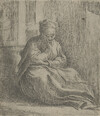
\includegraphics[keepaspectratio,width=0.6\textwidth]{thais-small.jpg}
  \captionart{MelancholieThais}
  \label{fig:thais}
\end{figure}

To see a fond mother, like Aesop's ape, hug her child to death, a
\authorfootnote{379}\worddef{a man who knows of his wife's infidelity and puts
up with it}{wittol} wink at his wife's honesty, and too perspicuous in all
other affairs; one stumble at a straw, and leap over a block; rob Peter, and
pay Paul; scrape unjust sums with one hand, purchase great manors by
corruption, fraud and \worddef{deception, trickery}{cozenage}, and liberally to
distribute to the poor with the other, give a remnant to pious uses, \etc{}
Penny wise, pound foolish; blind men judge of colours; wise men silent, fools
talk; \authorfootnote{380}find fault with others, and do worse themselves;
\authorfootnote{381}denounce that in public which he doth in secret; and which
Aurelius Victor gives out of Augustus, severely censure that in a third, of
which he is most guilty himself.

To see a poor fellow, or an hired servant venture his life for his new master
that will scarce give him his wages at year's end; A country colon toil and
moil, till and drudge for a prodigal idle drone, that devours all the gain, or
lasciviously consumes with fantastical expenses; A noble man in a bravado to
encounter death, and for a small flash of honour to cast away himself; A
worldling tremble at an executor, and yet not fear hell-fire; To wish and hope
for immortality, desire to be happy, and yet by all means avoid death, a
necessary passage to bring him to it.

To see a foolhardy fellow like those old Danes, \li{qui decollari malunt quam
verberari}, die rather than be punished, in a sottish humour embrace death with
alacrity, yet \authorfootnote{382}scorn to lament his own sins and miseries, or
his clearest friends' departures.

To see wise men degraded, fools preferred, one govern towns and cities, and yet
a silly woman overrules him at home; \authorfootnote{383}Command a province,
and yet his own servants or children prescribe laws to him, as Themistocles'
son did in Greece; \authorfootnote{384}"What I will" (said he) "my mother will,
and what my mother will, my father doth." To see horses ride in a coach, men
draw it; dogs devour their masters; towers build masons; children rule; old men
go to school; women wear the breeches; \authorfootnote{385}sheep demolish
towns, devour men, \etc{} And in a word, the world turned upside downward.
\li{O viveret Democritus}.

\authorfootnote{386}To insist in every particular were one of Hercules'
labours, there's so many ridiculous instances, as motes in the sun. \li{Quantum
est in rebus inane}? (How much vanity there is in things!) And who can speak of
all? \li{Crimine ab uno disce omnes}, take this for a taste.

But these are obvious to sense, trivial and well known, easy to be discerned.
How would Democritus have been moved, had he seen \authorfootnote{387}the
secrets of their hearts? If every man had a window in his breast, which Momus
would have had in Vulcan's man, or that which Tully so much wished it were
written in every man's forehead, \li{Quid quisque de republica sentiret}, what
he thought; or that it could be effected in an instant, which Mercury did by
Charon in Lucian, by touching of his eyes, to make him discern \li{semel et
simul rumores et susurros}.

\translatedverse{%
\begin{latin}
\begin{verse}%
Spes hominum caecas, morbos, votumque labores,\\*
Et passim toto volitantes aethere curas.\\!
\end{verse}%
\end{latin}}{%
\begin{verse}%
Blind hopes and wishes, their thoughts and affairs,\\*
Whispers and rumours, and those flying cares.\\!
\end{verse}}{}

That he could \li{cubiculorum obductas foras recludere et secreta cordium
penetrare}, which \authorfootnote{388}Cyprian desired, open doors and locks,
shoot bolts, as Lucian's Gallus did with a feather of his tail: or Gyges'
invisible ring, or some rare perspective glass, or \emph{Otacousticon}, which
would so multiply species, that a man might hear and see all at once (as
\authorfootnote{389}Martianus Capella's Jupiter did in a spear which he held in
his hand, which did present unto him all that was daily done upon the face of
the earth), observe cuckolds' horns, forgeries of alchemists, the philosopher's
stone, new projectors, \etc{}, and all those works of darkness, foolish vows,
hopes, fears and wishes, what a deal of laughter would it have afforded? He
should have seen windmills in one man's head, an hornet's nest in another. Or
had he been present with Icaromenippus in Lucian at Jupiter's whispering place,
\authorfootnote{390}and heard one pray for rain, another for fair weather; one
for his wife's, another for his father's death, \etc{}; "to ask that at God's
hand which they are abashed any man should hear:" How would he have been
confounded? Would he, think you, or any man else, say that these men were well
in their wits? \li{Haec sani esse hominis quis sanus juret Orestes}? Can all
the hellebore in the Anticyrae cure these men? No, sure,
\authorfootnote{391}"an acre of hellebore will not do it."

That which is more to be lamented, they are mad like Seneca's blind woman, and
will not acknowledge, or \authorfootnote{392}seek for any cure of it, for
\li{pauci vident morbum suum, omnes amant}. If our leg or arm offend us, we
covet by all means possible to redress it; \authorfootnote{393}and if we labour
of a bodily disease, we send for a physician; but for the diseases of the mind
we take no notice of them: \authorfootnote{394}Lust harrows us on the one side;
envy, anger, ambition on the other. We are torn in pieces by our passions, as
so many wild horses, one in disposition, another in habit; one is melancholy,
another mad; \authorfootnote{395}and which of us all seeks for help, doth
acknowledge his error, or knows he is sick? As that stupid fellow put out the
candle because the biting fleas should not find him; he shrouds himself in an
unknown habit, borrowed titles, because nobody should discern him. Every man
thinks with himself, \li{Egomet videor mihi sanus}, I am well, I am wise, and
laughs at others. And 'tis a general fault amongst them all, that
\authorfootnote{396}which our forefathers have approved, diet, apparel,
opinions, humours, customs, manners, we deride and reject in our time as
absurd. Old men account juniors all fools, when they are mere dizzards; and as
to sailors, ------ \li{terraeque urbesque recedunt} ------ they move, the land
stands still, the world hath much more wit, they dote themselves. Turks deride
us, we them; Italians Frenchmen, accounting them light headed fellows, the
French scoff again at Italians, and at their several customs; Greeks have
condemned all the world but themselves of barbarism, the world as much vilifies
them now; we account Germans heavy, dull fellows, explode many of their
fashions; they as contemptibly think of us; Spaniards laugh at all, and all
again at them. So are we fools and ridiculous, absurd in our actions,
carriages, diet, apparel, customs, and consultations; we
\authorfootnote{397}scoff and point one at another, when as in conclusion all
are fools, \authorfootnote{398}"and they the veriest asses that hide their ears
most." A private man if he be resolved with himself, or set on an opinion,
accounts all idiots and asses that are not affected as he is,
\authorfootnote{399}------ \li{nil rectum, nisi quod placuit sibi, ducit}, that
are not so minded, \authorfootnote{400}(\li{quodque volunt homines se bene
velle putant},) all fools that think not as he doth: he will not say with
Atticus, \li{Suam quisque sponsam, mihi meam}, let every man enjoy his own
spouse; but his alone is fair, \li{suus amor}, \etc{} and scorns all in respect
of himself \authorfootnote{401}will imitate none, hear none
\authorfootnote{402}but himself, as Pliny said, a law and example to himself.
And that which Hippocrates, in his epistle to Dionysius, reprehended of old, is
verified in our times, \li{Quisque in alio superfluum esse censet, ipse quod
non habet nec curat}, that which he hath not himself or doth not esteem, he
accounts superfluity, an idle quality, a mere foppery in another: like Aesop's
fox, when he had lost his tail, would have all his fellow foxes cut off theirs.
The Chinese say, that we Europeans have one eye, they themselves two, all the
world else is blind: (though \authorfootnote{403}Scaliger accounts them brutes
too, \li{merum pecus},) so thou and thy sectaries are only wise, others
indifferent, the rest beside themselves, mere idiots and asses. Thus not
acknowledging our own errors and imperfections, we securely deride others, as
if we alone were free, and spectators of the rest, accounting it an excellent
thing, as indeed it is, \li{Aliena optimum frui insania}, to make ourselves
merry with other men's obliquities, when as he himself is more faulty than the
rest, \li{mutato nomine, de te fabula narratur}, he may take himself by the
nose for a fool; and which one calls \li{maximum stultitiae specimen}, to be
ridiculous to others, and not to perceive or take notice of it, as Marsyas was
when he contended with Apollo, \li{non intelligens se deridiculo haberi}, saith
\authorfootnote{404}Apuleius; 'tis his own cause, he is a convicted madman, as
\authorfootnote{405}Austin well infers "in the eyes of wise men and angels he
seems like one, that to our thinking walks with his heels upwards." So thou
laughest at me, and I at thee, both at a third; and he returns that of the poet
upon us again, \authorfootnote{406}\li{Hei mihi, insanire me aiunt, quum ipsi
ultro insaniant}. We accuse others of madness, of folly, and are the veriest
dizzards ourselves. For it is a great sign and property of a fool (which
\biblecite{Eccl. \rn{x.} 3}, points at) out of pride and self-conceit to insult,
vilify, condemn, censure, and call other men fools (\li{Non videmus manticae
quod a tergo est}) to tax that in others of which we are most faulty; teach
that which we follow not ourselves: For an inconstant man to write of
constancy, a profane liver prescribe rules of sanctity and piety, a dizzard
himself make a treatise of wisdom, or with Sallust to rail downright at
spoilers of countries, and yet in \authorfootnote{407}office to be a most
grievous poller himself. This argues weakness, and is an evident sign of such
parties' indiscretion. \authorfootnote{408}\li{Peccat uter nostrum cruce
dignius}? "Who is the fool now?" Or else peradventure in some places we are all
mad for company, and so 'tis not seen, \li{Satietas erroris et dementiae,
pariter absurditatem et admirationem tollit}. 'Tis with us, as it was of old
(in \authorfootnote{409}Tully's censure at least) with C. Pimbria in Rome, a
bold, hair-brain, mad fellow, and so esteemed of all, such only excepted, that
were as mad as himself: now in such a case there is \authorfootnote{410}no
notice taken of it.

\translatedverse{%
\begin{latin}
\begin{verse}%
Nimirum insanus paucis videatur; eo quod\\*
Maxima pars hominum morbo jactatur eodem.\\!
\end{verse}%
\end{latin}}{%
\begin{verse}%
When all are mad, where all are like opprest\\*
Who can discern one mad man from the rest?\\!
\end{verse}}{}

But put case they do perceive it, and some one be manifestly convicted of
madness, \authorfootnote{411}he now takes notice of his folly, be it in action,
gesture, speech, a vain humour he hath in building, bragging, jangling,
spending, gaming, courting, scribbling, prating, for which he is ridiculous to
others, \authorfootnote{412}on which he dotes, he doth acknowledge as much: yet
with all the rhetoric thou hast, thou canst not so recall him, but to the
contrary notwithstanding, he will persevere in his dotage. 'Tis \li{amabilis
insania, et mentis gratissimus error}, so pleasing, so delicious, that he
\authorfootnote{413}cannot leave it. He knows his error, but will not seek to
decline it, tell him what the event will be, beggary, sorrow, sickness,
disgrace, shame, loss, madness, yet \authorfootnote{414}"an angry man will
prefer vengeance, a lascivious his whore, a thief his booty, a glutton his
belly, before his welfare." Tell an epicure, a covetous man, an ambitious man
of his irregular course, wean him from it a little, \li{pol me occidistis
amici}, he cries anon, you have undone him, and as \authorfootnote{415}a "dog
to his vomit," he returns to it again; no persuasion will take place, no
counsel, say what thou canst,

\translatedverse{%
\begin{latin}
\begin{verse}%
Clames licet et mare coelo\\*
------Confundas, surdo narras,\\!
\end{verse}%
\end{latin}}{%\setauthornote{416}
\begin{verse}%
Although you call out, and confound the sea and sky,\\*
you still address a deaf man.\\!
\end{verse}}{}

demonstrate as Ulysses did to \authorfootnote{417}Elpenor and Gryllus, and the
rest of his companions "those swinish men," he is irrefragable in his humour,
he will be a hog still; bray him in a mortar, he will be the same. If he be in
an heresy, or some perverse opinion, settled as some of our ignorant Papists
are, convince his understanding, show him the several follies and absurd
fopperies of that sect, force him to say, \li{veris vincor}, make it as clear
as the sun, \authorfootnote{418}he will err still, peevish and obstinate as he
is; and as he said \authorfootnote{419}\li{si in hoc erro, libenter erro, nec
hunc errorem auferri mihi volo}; I will do as I have done, as my predecessors
have done, \authorfootnote{420}and as my friends now do: I will dote for
company. Say now, are these men \authorfootnote{421}mad or no,
\authorfootnote{422}\li{Heus age responde}? are they ridiculous? \li{cedo
quemvis arbitrum}, are they \li{sanae mentis}, sober, wise, and discreet? have
they common sense? ------ \authorfootnote{423}\li{uter est insanior horum}? I
am of Democritus' opinion for my part, I hold them worthy to be laughed at; a
company of brain-sick dizzards, as mad as \authorfootnote{424}Orestes and
Athamas, that they may go "ride the ass," and all sail along to the Anticyrae,
in the "ship of fools" for company together. I need not much labour to prove
this which I say otherwise than thus, make any solemn protestation, or swear, I
think you will believe me without an oath; say at a word, are they fools? I
refer it to you, though you be likewise fools and madmen yourselves, and I as
mad to ask the question; for what said our comical Mercury?

\translatedverse{%
\begin{latin}
\begin{verse}%
Justum ab injustis petere insipientia est.\\!
\end{verse}%
\end{latin}}{%
\begin{verse}%
I'll stand to your censure yet, what think you?\\!
\end{verse}}{%
\attrib{\getauthornote{425}}}

But forasmuch as I undertook at first, that kingdoms, provinces, families, were
melancholy as well as private men, I will examine them in particular, and that
which I have hitherto dilated at random, in more general terms, I will
particularly insist in, prove with more special and evident arguments,
testimonies, illustrations, and that in brief. \authorfootnote{426}\li{Nunc
accipe quare desipiant omnes aeque ac tu.} My first argument is borrowed from
Solomon, an arrow drawn out of his sententious quiver, \biblecite{Pro. \rn{iii.}
7}, "Be not wise in thine own eyes." And \biblecite{xxvi. 12}, "Seest thou a man
wise in his own conceit? more hope is of a fool than of him." Isaiah
pronounceth a woe against such men, \biblecite{cap. \rn{v.} 21}, "that are wise
in their own eyes, and prudent in their own sight." For hence we may gather,
that it is a great offence, and men are much deceived that think too well of
themselves, an especial argument to convince them of folly. Many men (saith
\authorfootnote{427}Seneca) "had been without question wise, had they not had
an opinion that they had attained to perfection of knowledge already, even
before they had gone half way," too forward, too ripe, \li{praeproperi}, too
quick and ready, \authorfootnote{428}\li{cito prudentes, cito pii, cito mariti,
cito patres, cito sacerdotes, cito omnis officii capaces et curiosi}, they had
too good a conceit of themselves, and that marred all; of their worth, valour,
skill, art, learning, judgment, eloquence, their good parts; all their geese
are swans, and that manifestly proves them to be no better than fools. In
former times they had but seven wise men, now you can scarce find so many
fools. Thales sent the golden tripos, which the fishermen found, and the oracle
commanded to be \authorfootnote{429}"given to the wisest, to Bias, Bias to
Solon," \etc{} If such a thing were now found, we should all fight for it, as
the three goddesses did for the golden apple, we are so wise: we have women
politicians, children metaphysicians; every silly fellow can square a circle,
make perpetual motions, find the philosopher's stone, interpret Apocalypses,
make new Theories, a new system of the world, new Logic, new Philosophy, \etc{}
\li{Nostra utique regio}, saith \authorfootnote{430}Petronius, "our country is
so full of deified spirits, divine souls, that you may sooner find a God than a
man amongst us," we think so well of ourselves, and that is an ample testimony
of much folly.

My second argument is grounded upon the like place of Scripture, which though
before mentioned in effect, yet for some reasons is to be repeated (and by
Plato's good leave, I may do it, \authorfootnote{431}\textgreek{δίς τὸ καλὸν
ρηθέν ὀυδέν βλάπτει}) "Fools" (saith David) "by reason of their
transgressions." \etc{} \biblecite{Psal. \rn{cvii.} 17}. Hence Musculus infers
all transgressors must needs be fools. So we read \biblecite{Rom. \rn{ii.}},
"Tribulation and anguish on the soul of every man that doeth evil;" but all do
evil. And \biblecite{Isaiah, \rn{lxv.} 14}, "My servant shall sing for joy, and
\authorfootnote{432}ye shall cry for sorrow of heart, and vexation of mind."
'Tis ratified by the common consent of all philosophers. "Dishonesty" (saith
Cardan) "is nothing else but folly and madness." \li{Probus quis nobiscum
vivit?}\authorlatintrans{433.5}\authormarginnote{433} Show me an honest man,
\li{Nemo malus qui non stultus}, 'tis Fabius' aphorism to the same end. If none
honest, none wise, then all fools. And well may they be so accounted: for who
will account him otherwise, \li{Qui iter adornat in occidentem, quum properaret
in orientem}? that goes backward all his life, westward, when he is bound to
the east? or hold him a wise man (saith \authorfootnote{434}Musculus) "that
prefers momentary pleasures to eternity, that spends his master's goods in his
absence, forthwith to be condemned for it?" \li{Nequicquam sapit qui sibi non
sapit}, who will say that a sick man is wise, that eats and drinks to overthrow
the temperature of his body? Can you account him wise or discreet that would
willingly have his health, and yet will do nothing that should procure or
continue it? \authorfootnote{435}Theodoret, out of Plotinus the Platonist,
"holds it a ridiculous thing for a man to live after his own laws, to do that
which is offensive to God, and yet to hope that he should save him: and when he
voluntarily neglects his own safety, and contemns the means, to think to be
delivered by another:" who will say these men are wise?

A third argument may be derived from the precedent, \authorfootnote{436}all men
are carried away with passion, discontent, lust, pleasures, \etc{}, they
generally hate those virtues they should love, and love such vices they should
hate. Therefore more than melancholy, quite mad, brute beasts, and void of
reason, so Chrysostom contends; "or rather dead and buried alive," as
\authorfootnote{437}Philo Judeus concludes it for a certainty, "of all such
that are carried away with passions, or labour of any disease of the mind.
Where is fear and sorrow," there \authorfootnote{438}Lactantius stiffly
maintains, "wisdom cannot dwell,"

\translatedverse{%
\begin{latin}
\begin{verse}%
------qui cupiet, metuet quoque porro,\\*
Qui metuens vivit, liber mihi non erit unquam.\\!
\end{verse}%
\end{latin}}{%\authorfootnote{439}
\begin{verse}%
He who is desirous is also fearful,\\*
and he who lives in fear never can be free.\\!
\end{verse}}{}

Seneca and the rest of the stoics are of opinion, that where is any the least
perturbation, wisdom may not be found. "What more ridiculous," as
\authorfootnote{440}Lactantius urges, than to hear how Xerxes whipped the
Hellespont, threatened the Mountain Athos, and the like. To speak \li{ad rem},
who is free from passion? \authorfootnote{441}\li{Mortalis nemo est quem non
attingat dolor, morbusve}, as \authorfootnote{442}Tully determines out of an
old poem, no mortal men can avoid sorrow and sickness, and sorrow is an
inseparable companion from melancholy. \authorfootnote{443}Chrysostom pleads
farther yet, that they are more than mad, very beasts, stupefied and void of
common sense: "For how" (saith he) "shall I know thee to be a man, when thou
kickest like an ass, neighest like a horse after women, ravest in lust like a
bull, ravenest like a bear, stingest like a scorpion, rakest like a wolf, as
subtle as a fox, as impudent as a dog? Shall I say thou art a man, that hast
all the symptoms of a beast? How shall I know thee to be a man? by thy shape?
That affrights me more, when I see a beast in likeness of a man."

\authorfootnote{444}Seneca calls that of Epicurus, \li{magnificam vocem}, an
heroical speech, "A fool still begins to live," and accounts it a filthy
lightness in men, every day to lay new foundations of their life, but who doth
otherwise? One travels, another builds; one for this, another for that
business, and old folks are as far out as the rest; \li{O dementem senectutem},
Tully exclaims. Therefore young, old, middle age, are all stupid, and dote.

\authorfootnote{445}Aeneas Sylvius, amongst many other, sets down three special
ways to find a fool by. He is a fool that seeks that he cannot find: he is a
fool that seeks that, which being found will do him more harm than good: he is
a fool, that having variety of ways to bring him to his journey's end, takes
that which is worst. If so, methinks most men are fools; examine their courses,
and you shall soon perceive what dizzards and mad men the major part are.

Beroaldus will have drunkards, afternoon men, and such as more than ordinarily
delight in drink, to be mad. The first pot quencheth thirst, so Panyasis the
poet determines in \li{Athenaeus, secunda gratiis, horis et Dyonisio}: the
second makes merry, the third for pleasure, \li{quarta, ad insaniam}, the
fourth makes them mad. If this position be true, what a catalogue of mad men
shall we have? what shall they be that drink four times four? \li{Nonne supra
omnem furorem, supra omnem insanian reddunt insanissimos}? I am of his opinion,
they are more than mad, much worse than mad.

The \authorfootnote{446}Abderites condemned Democritus for a mad man, because
he was sometimes sad, and sometimes again profusely merry. \li{Hac Patria}
(saith Hippocrates) \li{ob risum furere et insanire dicunt}, his countrymen
hold him mad because he laughs; \authorfootnote{447}and therefore "he desires
him to advise all his friends at Rhodes, that they do not laugh too much, or be
over sad." Had those Abderites been conversant with us, and but seen what
\authorfootnote{448}fleering and grinning there is in this age, they would
certainly have concluded, we had been all out of our wits.

Aristotle in his Ethics holds \li{felix idemque sapiens}, to be wise and happy,
are reciprocal terms, \li{bonus idemque sapiens honestus}. 'Tis
\authorfootnote{449}Tully's paradox, "wise men are free, but fools are slaves,"
liberty is a power to live according to his own laws, as we will ourselves: who
hath this liberty? who is free?

\translatedverse{%
\begin{latin}
\begin{verse}%
------sapiens sibique imperiosus,\\*
Quem neque pauperis, neque mors, neque vincula terrent,\\*
Responsare cupidinibus, contemnere honores\\*
Fortis, et in seipso totus teres atque rotundus.\\!
\end{verse}%
\end{latin}}{%
\begin{verse}%
He is wise that can command his own will,\\*
Valiant and constant to himself still,\\*
Whom poverty nor death, nor bands can fright,\\*
Checks his desires, scorns honours, just and right.\\!
\end{verse}}{%
\attrib{\getauthornote{450}}}

But where shall such a man be found? If no where, then \li{e diametro}, we are
all slaves, senseless, or worse. \li{Nemo malus felix}. But no man is happy in
this life, none good, therefore no man wise. \authorfootnote{451}\li{Rari
quippe boni------}\authorlatintrans{451.5}\authormarginnote{451} For one virtue
you shall find ten vices in the same party; \li{pauci Promethei, multi
Epimethei}. We may peradventure usurp the name, or attribute it to others for
favour, as Carolus Sapiens, Philippus Bonus, Lodovicus Pius, \etc{}, and
describe the properties of a wise man, as Tully doth an orator, Xenophon Cyrus,
Castilio a courtier, Galen temperament, an aristocracy is described by
politicians. But where shall such a man be found?

\translatedverse{%
\begin{latin}
\begin{verse}%
Vir bonus et sapiens, qualem vix repperit unum\\*
Millibus e multis hominum consultus Apollo.\\!
\end{verse}%
\end{latin}}{%
\begin{verse}%
A wise, a good man in a million,\\*
Apollo consulted could scarce find one.\\!
\end{verse}}{}

A man is a miracle of himself, but Trismegistus adds, \li{Maximum miraculum
homo sapiens}, a wise man is a wonder: \li{multi Thirsigeri, pauci Bacchi}.

Alexander when he was presented with that rich and costly casket of king
Darius, and every man advised him what to put in it, he reserved it to keep
Homer's works, as the most precious jewel of human wit, and yet
\authorfootnote{452}Scaliger upbraids Homer's muse, \li{Nutricem insanae
sapientiae}, a nursery of madness, \authorfootnote{453}impudent as a court
lady, that blushes at nothing. Jacobus Mycillus, Gilbertus Cognatus, Erasmus,
and almost all posterity admire Lucian's luxuriant wit, yet Scaliger rejects
him in his censure, and calls him the Cerberus of the muses. Socrates, whom all
the world so much magnified, is by Lactantius and Theodoret condemned for a
fool. Plutarch extols Seneca's wit beyond all the Greeks, \li{nulli secundus},
yet \authorfootnote{454}Seneca saith of himself, "when I would solace myself
with a fool, I reflect upon myself, and there I have him." Cardan, in his
Sixteenth Book of Subtleties, reckons up twelve supereminent, acute
philosophers, for worth, subtlety, and wisdom: Archimedes, Galen, Vitruvius,
Architas Tarentinus, Euclid, Geber, that first inventor of Algebra, Alkindus
the Mathematician, both Arabians, with others. But his \li{triumviri terrarum}
far beyond the rest, are Ptolomaeus, Plotinus, Hippocrates. Scaliger
\bookcite{\textlatin{exercitat. 224}}, scoffs at this censure of his, calls
some of them carpenters and mechanicians, he makes Galen \li{fimbriam
Hippocratis}, a skirt of Hippocrates: and the said \authorfootnote{455}Cardan
himself elsewhere condemns both Galen and Hippocrates for tediousness,
obscurity, confusion. Paracelsus will have them both mere idiots, infants in
physic and philosophy. Scaliger and Cardan admire Suisset the Calculator,
\li{qui pene modum excessit humani ingenii}, and yet \authorfootnote{456}Lod.
Vives calls them \li{nugas Suisseticas}: and Cardan, opposite to himself in
another place, contemns those ancients in respect of times present,
\authorfootnote{457}\li{Majoresque nostros ad presentes collatos juste pueros
appellari}. In conclusion, the said \authorfootnote{458}Cardan and Saint
Bernard will admit none into this catalogue of wise men,
\authorfootnote{459}but only prophets and apostles; how they esteem themselves,
you have heard before. We are worldly-wise, admire ourselves, and seek for
applause: but hear Saint \authorfootnote{460}Bernard, \li{quanto magis foras es
sapiens, tanto magis intus stultus efficeris}, \etc{} \li{in omnibus es
prudens, circa teipsum insipiens}: the more wise thou art to others, the more
fool to thyself. I may not deny but that there is some folly approved, a divine
fury, a holy madness, even a spiritual drunkenness in the saints of God
themselves; \li{sanctum insanium} Bernard calls it (though not as blaspheming
\authorfootnote{461}Vorstius, would infer it as a passion incident to God
himself, but) familiar to good men, as that of Paul, \biblecite{2 Cor.} "he was a
fool," \etc{} and \biblecite{Rom. \rn{ix.}} he wisheth himself to be
anathematised for them. Such is that drunkenness which Ficinus speaks of, when
the soul is elevated and ravished with a divine taste of that heavenly nectar,
which poets deciphered by the sacrifice of Dionysius, and in this sense with
the poet, \authorfootnote{462}\li{insanire lubet}, as Austin exhorts us, \li{ad
ebrietatem se quisque paret}, let's all be mad and \authorfootnote{463}drunk.
But we commonly mistake, and go beyond our commission, we reel to the opposite
part, \authorfootnote{464}we are not capable of it, \authorfootnote{465}and as
he said of the Greeks, \li{Vos Graeci semper pueri, vos Britanni, Galli,
Germani, Itali}, \etc{} you are a company of fools.

Proceed now \li{a partibus ad totum}, or from the whole to parts, and you shall
find no other issue, the parts shall be sufficiently dilated in this following
Preface. The whole must needs follow by a sorites or induction. Every multitude
is mad, \authorfootnote{466}\li{bellua multorum capitum}, (a many-headed
beast), precipitate and rash without judgment, \li{stultum animal}, a roaring
rout. \authorfootnote{467}Roger Bacon proves it out of Aristotle, \li{Vulgus
dividi in oppositum contra sapientes, quod vulgo videtur verum, falsum est};
that which the commonalty accounts true, is most part false, they are still
opposite to wise men, but all the world is of this humour (\li{vulgus}), and
thou thyself art \li{de vulgo}, one of the commonalty; and he, and he, and so
are all the rest; and therefore, as Phocion concludes, to be approved in nought
you say or do, mere idiots and asses. Begin then where you will, go backward or
forward, choose out of the whole pack, wink and choose, you shall find them all
alike, "never a barrel better herring."

Copernicus, Atlas his successor, is of opinion, the earth is a planet, moves
and shines to others, as the moon doth to us. Digges, Gilbert, Keplerus,
Origanus, and others, defend this hypothesis of his in sober sadness, and that
the moon is inhabited: if it be so that the earth is a moon, then are we also
giddy, vertiginous and lunatic within this sublunary maze.

I could produce such arguments till dark night: if you should hear the rest,

\translatedverse{%
\begin{latin}
\begin{verse}%
Ante diem clauso component vesper Olimpo:\\!
\end{verse}%
\end{latin}}{%
\begin{verse}%
Through such a train of words if I should run,\\*
The day would sooner than the tale be done:\\!
\end{verse}}{}

but according to my promise, I will descend to particulars. This melancholy
extends itself not to men only, but even to vegetals and sensibles. I speak not
of those creatures which are saturnine, melancholy by nature, as lead, and such
like minerals, or those plants, rue, cypress, \etc{} and hellebore itself, of
which \authorfootnote{468}Agrippa treats, fishes, birds, and beasts, hares,
conies, dormice, \etc{}, owls, bats, nightbirds, but that artificial, which is
perceived in them all. Remove a plant, it will pine away, which is especially
perceived in date trees, as you may read at large in Constantine's husbandry,
that antipathy betwixt the vine and the cabbage, vine and oil. Put a bird in a
cage, he will die for sullenness, or a beast in a pen, or take his young ones
or companions from him, and see what effect it will cause. But who perceives
not these common passions of sensible creatures, fear, sorrow, \etc{} Of all
other, dogs are most subject to this malady, insomuch some hold they dream as
men do, and through violence of melancholy run mad; I could relate many stories
of dogs that have died for grief, and pined away for loss of their masters, but
they are common in every \authorfootnote{469}author.

Kingdoms, provinces, and politic bodies are likewise sensible and subject to
this disease, as \authorfootnote{470}Boterus in his politics hath proved at
large. "As in human bodies" (saith he) "there be divers alterations proceeding
from humours, so be there many diseases in a commonwealth, which do as
diversely happen from several distempers," as you may easily perceive by their
particular symptoms. For where you shall see the people civil, obedient to God
and princes, judicious, peaceable and quiet, rich, fortunate,
\authorfootnote{471}and flourish, to live in peace, in unity and concord, a
country well tilled, many fair built and populous cities, \li{ubi incolae
nitent} as old \authorfootnote{472}Cato said, the people are neat, polite and
terse, \li{ubi bene, beateque vivunt}, which our politicians make the chief end
of a commonwealth; and which \authorfootnote{473}Aristotle,
\bookcite{\textlatin{Polit. lib. 3, cap. 4}}, calls \li{Commune bonum},
Polybius \bookcite{\textlatin{lib. 6}}, \li{optabilem et selectum statum}, that
country is free from melancholy; as it was in Italy in the time of Augustus,
now in China, now in many other flourishing kingdoms of Europe. But whereas you
shall see many discontents, common grievances, complaints, poverty, barbarism,
beggary, plagues, wars, rebellions, seditions, mutinies, contentions, idleness,
riot, epicurism, the land lie untilled, waste, full of bogs, fens, deserts,
\etc{}, cities decayed, base and poor towns, villages depopulated, the people
squalid, ugly, uncivil; that kingdom, that country, must needs be discontent,
melancholy, hath a sick body, and had need to be reformed.

Now that cannot well be effected, till the causes of these maladies be first
removed, which commonly proceed from their own default, or some accidental
inconvenience: as to be situated in a bad clime, too far north, sterile, in a
barren place, as the desert of Libya, deserts of Arabia, places void of waters,
as those of Lop and Belgian in Asia, or in a bad air, as at Alexandretta,
Bantam, Pisa, Durrazzo, S. John de Ulloa, \etc{}, or in danger of the sea's
continual inundations, as in many places of the Low Countries and elsewhere, or
near some bad neighbours, as Hungarians to Turks, Podolians to Tartars, or
almost any bordering countries, they live in fear still, and by reason of
hostile incursions are oftentimes left desolate. So are cities by reason
\authorfootnote{474}of wars, fires, plagues, inundations,
\authorfootnote{475}wild beasts, decay of trades, barred havens, the sea's
violence, as Antwerp may witness of late, Syracuse of old, Brundusium in Italy,
Rye and Dover with us, and many that at this day suspect the sea's fury and
rage, and labour against it as the Venetians to their inestimable charge. But
the most frequent maladies are such as proceed from themselves, as first when
religion and God's service is neglected, innovated or altered, where they do
not fear God, obey their prince, where atheism, epicurism, sacrilege, simony,
\etc{}, and all such impieties are freely committed, that country cannot
prosper. When Abraham came to Gerar, and saw a bad land, he said, sure the fear
of God was not in that place. \authorfootnote{476}Cyprian Echovius, a Spanish
chorographer, above all other cities of Spain, commends Borcino, "in which
there was no beggar, no man poor, \etc{}, but all rich, and in good estate, and
he gives the reason, because they were more religious than, their neighbours:"
why was Israel so often spoiled by their enemies, led into captivity, \etc{},
but for their idolatry, neglect of God's word, for sacrilege, even for one
Achan's fault? And what shall we except that have such multitudes of Achans,
church robbers, simoniacal patrons, \etc{}, how can they hope to flourish, that
neglect divine duties, that live most part like Epicures?

Other common grievances are generally noxious to a body politic; alteration of
laws and customs, breaking privileges, general oppressions, seditions, \etc{},
observed by \authorfootnote{477}Aristotle, Bodin, Boterus, Junius, Arniscus,
\etc{} I will only point at some of chiefest.
\authorfootnote{478}\li{Impotentia gubernandi, ataxia}, confusion, ill
government, which proceeds from unskilful, slothful, griping, covetous, unjust,
rash, or tyrannizing magistrates, when they are fools, idiots, children, proud,
wilful, partial, indiscreet, oppressors, giddy heads, tyrants, not able or
unfit to manage such offices: \authorfootnote{479}many noble cities and
flourishing kingdoms by that means are desolate, the whole body groans under
such heads, and all the members must needs be disaffected, as at this day those
goodly provinces in Asia Minor, \etc{} groan under the burthen of a Turkish
government; and those vast kingdoms of Muscovia, Russia,
\authorfootnote{480}under a tyrannizing duke. Who ever heard of more civil and
rich populous countries than those of "Greece, Asia Minor, abounding with all
\authorfootnote{481}wealth, multitudes of inhabitants, force, power, splendour
and magnificence?" and that miracle of countries, \authorfootnote{482}the Holy
Land, that in so small a compass of ground could maintain so many towns,
cities, produce so many fighting men? Egypt another paradise, now barbarous and
desert, and almost waste, by the despotical government of an imperious Turk,
\li{intolerabili servitutis jugo premitur} (\authorfootnote{483}one saith) not
only fire and water, goods or lands, \li{sed ipse spiritus ab insolentissimi
victoris pendet nutu}, such is their slavery, their lives and souls depend upon
his insolent will and command. A tyrant that spoils all wheresoever he comes,
insomuch that an \authorfootnote{484}historian complains, "if an old inhabitant
should now see them, he would not know them, if a traveller, or stranger, it
would grieve his heart to behold them." Whereas \authorfootnote{485}Aristotle
notes, \li{Novae exactiones, nova onera imposita}, new burdens and exactions
daily come upon them, like those of which Zosimus, \bookcite{\textlatin{lib.
2}}, so grievous, \li{ut viri uxores, patres filios prostituerent ut
exactoribus e questu}, \etc{}, they must needs be discontent, \li{hinc
civitatum gemitus et ploratus}, as \authorfootnote{486}Tully holds, hence come
those complaints and tears of cities, "poor, miserable, rebellious, and
desperate subjects," as \authorfootnote{487}Hippolitus adds; and
\authorfootnote{488}as a judicious countryman of ours observed not long since,
in a survey of that great Duchy of Tuscany, the people lived much grieved and
discontent, as appeared by their manifold and manifest complainings in that
kind. "That the state was like a sick body which had lately taken physic, whose
humours are not yet well settled, and weakened so much by purging, that nothing
was left but melancholy."

Whereas the princes and potentates are immoderate in lust, hypocrites,
epicures, of no religion, but in show: \li{Quid hypocrisi fragilius}? what so
brittle and unsure? what sooner subverts their estates than wandering and
raging lusts, on their subjects' wives, daughters? to say no worse. That they
should \li{facem praeferre}, lead the way to all virtuous actions, are the
ringleaders oftentimes of all mischief and dissolute courses, and by that means
their countries are plagued, \authorfootnote{489}"and they themselves often
ruined, banished, or murdered by conspiracy of their subjects, as Sardanapalus
was, Dionysius Junior, Heliogabalus, Periander, Pisistratus, Tarquinius,
Timocrates, Childericus, Appius Claudius, Andronicus, Galeacius Sforza,
Alexander Medices," \etc{}

Whereas the princes or great men are malicious, envious, factious, ambitious,
emulators, they tear a commonwealth asunder, as so many Guelfs and Gibelines
disturb the quietness of it, \authorfootnote{490}and with mutual murders let it
bleed to death; our histories are too full of such barbarous inhumanities, and
the miseries that issue from them.

Whereas they be like so many horseleeches, hungry, griping, corrupt,
\authorfootnote{491}covetous, \li{avaritice mancipia}, ravenous as wolves, for
as Tully writes: \li{qui praeest prodest, et qui pecudibus praeest, debet eorum
utilitati inservire}: or such as prefer their private before the public good.
For as \authorfootnote{492}he said long since, \li{res privatae publicis semper
officere}. Or whereas they be illiterate, ignorant, empirics in policy, \li{ubi
deest facultas}, \authorfootnote{493}\li{virtus} (Aristot.
\bookcite{\textlatin{pol. 5, cap. 8.}}) \li{et scientia}, wise only by
inheritance, and in authority by birthright, favour, or for their wealth and
titles; there must needs be a fault, \authorfootnote{494}a great defect:
because as an \authorfootnote{495}old philosopher affirms, such men are not
always fit. "Of an infinite number, few alone are senators, and of those few,
fewer good, and of that small number of honest, good, and noble men, few that
are learned, wise, discreet and sufficient, able to discharge such places, it
must needs turn to the confusion of a state."

For as the \authorfootnote{496}Princes are, so are the people; \li{Qualis Rex,
talis grex}: and which \authorfootnote{497}Antigonus right well said of old,
\li{qui Macedonia regem erudit, omnes etiam subditos erudit}, he that teacheth
the king of Macedon, teacheth all his subjects, is a true saying still.

\begin{verse}%
For Princes are the glass, the school, the book,\\*
Where subjects' eyes do learn, do read, do look.\\!
\end{verse}%

\translatedverse{%
\begin{latin}
\begin{verse}%
------Velocius et citius nos\\*
Corrumpunt vitiorum exempla domestica, magnis\\*
Cum subeant animos auctoribus.------\\!
\end{verse}%
\end{latin}}{%\setauthornote{498}
\begin{verse}%
Vicious domestic examples operate more quickly\\*
upon us when suggested to our minds\\*
by high authorities.\\!
\end{verse}}{}

Their examples are soonest followed, vices entertained, if they be profane,
irreligious, lascivious, riotous, epicures, factious, covetous, ambitious,
illiterate, so will the commons most part be, idle, unthrifts, prone to lust,
drunkards, and therefore poor and needy (\textgreek{ἡ πενια στάσιν ἐμποιει καὶ
κακουργίαν}, for poverty begets sedition and villainy) upon all occasions ready
to mutiny and rebel, discontent still, complaining, murmuring, grudging, apt to
all outrages, thefts, treasons, murders, innovations, in debt, shifters,
cozeners, outlaws, \li{Profligatae famae ac vitae}. It was an old
\authorfootnote{499}politician's aphorism, "They that are poor and bad envy
rich, hate good men, abhor the present government, wish for a new, and would
have all turned topsy-turvy." When Catiline rebelled in Rome, he got a company
of such debauched rogues together, they were his familiars and coadjutors, and
such have been your rebels most part in all ages, Jack Cade, Tom Straw, Kette,
and his companions.

Where they be generally riotous and contentious, where there be many discords,
many laws, many lawsuits, many lawyers and many physicians, it is a manifest
sign of a distempered, melancholy state, as \authorfootnote{500}Plato long
since maintained: for where such kind of men swarm, they will make more work
for themselves, and that body politic diseased, which was otherwise sound. A
general mischief in these our times, an insensible plague, and never so many of
them: "which are now multiplied" (saith Mat. Geraldus, \authorfootnote{501}a
lawyer himself,) "as so many locusts, not the parents, but the plagues of the
country, and for the most part a supercilious, bad, covetous, litigious
generation of men." \authorfootnote{502}\li{Crumenimulga natio} \etc{} A
purse-milking nation, a clamorous company, gowned vultures,
\authorfootnote{503}\li{qui ex injuria vivent et sanguine civium}, thieves and
seminaries of discord; worse than any pollers by the highway side, \li{auri
accipitres, auri exterebronides, pecuniarum hamiolae, quadruplatores, curiae
harpagones, fori tintinabula, monstra hominum, mangones}, \etc{} that take upon
them to make peace, but are indeed the very disturbers of our peace, a company
of irreligious harpies, scraping, griping catchpoles, (I mean our common hungry
pettifoggers, \authorfootnote{504}\li{rabulas forenses}, love and honour in the
meantime all good laws, and worthy lawyers, that are so many
\authorfootnote{505}oracles and pilots of a well-governed commonwealth).
Without art, without judgment, that do more harm, as \authorfootnote{506}Livy
said, \li{quam bella externa, fames, morbive}, than sickness, wars, hunger,
diseases; "and cause a most incredible destruction of a commonwealth," saith
\authorfootnote{507}Sesellius, a famous civilian sometimes in Paris, as ivy
doth by an oak, embrace it so long, until it hath got the heart out of it, so
do they by such places they inhabit; no counsel at all, no justice, no speech
to be had, \li{nisi eum premulseris}, he must be fed still, or else he is as
mute as a fish, better open an oyster without a knife. \li{Experto crede}
(saith \authorfootnote{508}Salisburiensis) \li{in manus eorum millies incidi,
et Charon immitis qui nulli pepercit unquam, his longe clementior est}; "I
speak out of experience, I have been a thousand times amongst them, and Charon
himself is more gentle than they; \authorfootnote{509}he is contented with his
single pay, but they multiply still, they are never satisfied," besides they
have \li{damnificas linguas}, as he terms it, \li{nisi funibus argenteis
vincias}, they must be fed to say nothing, and \authorfootnote{510}get more to
hold their peace than we can to say our best. They will speak their clients
fair, and invite them to their tables, but as he follows it,
\authorfootnote{511}"of all injustice there is none so pernicious as that of
theirs, which when they deceive most, will seem to be honest men." They take
upon them to be peacemakers, \li{et fovere causas humilium}, to help them to
their right, \li{patrocinantur afflictis}, \authorfootnote{512}but all is for
their own good, \li{ut loculos pleniorom exhauriant}, they plead for poor men
gratis, but they are but as a stale to catch others. If there be no jar,
\authorfootnote{513}they can make a jar, out of the law itself find still some
quirk or other, to set them at odds, and continue causes so long, \li{lustra
aliquot}, I know not how many years before the cause is heard, and when 'tis
judged and determined by reason of some tricks and errors, it is as fresh to
begin, after twice seven years sometimes, as it was at first; and so they
prolong time, delay suits till they have enriched themselves, and beggared
their clients. And, as \authorfootnote{514}Cato inveighed against Isocrates'
scholars, we may justly tax our wrangling lawyers, they do \li{consenescere in
litibus}, are so litigious and busy here on earth, that I think they will plead
their client's causes hereafter, some of them in hell.
\authorfootnote{515}Simlerus complains amongst the Swissers of the advocates in
his time, that when they should make an end, they began controversies, and
"protract their causes many years, persuading them their title is good, till
their patrimonies be consumed, and that they have spent more in seeking than
the thing is worth, or they shall get by the recovery." So that he that goes to
law, as the proverb is, \authorfootnote{516}holds a wolf by the ears, or as a
sheep in a storm runs for shelter to a brier, if he prosecute his cause he is
consumed, if he surcease his suit he loseth all; \authorfootnote{517}what
difference? They had wont heretofore, saith Austin, to end matters, \li{per
communes arbitros}; and so in Switzerland (we are informed by
\authorfootnote{518}Simlerus), "they had some common arbitrators or daysmen in
every town, that made a friendly composition betwixt man and man, and he much
wonders at their honest simplicity, that could keep peace so well, and end such
great causes by that means." At \authorfootnote{519}Fez in Africa, they have
neither lawyers nor advocates; but if there be any controversies amongst them,
both parties plaintiff and defendant come to their Alfakins or chief judge,
"and at once without any farther appeals or pitiful delays, the cause is heard
and ended." Our forefathers, as \authorfootnote{520}a worthy chorographer of
ours observes, had wont \li{pauculis cruculis aureis}, with a few golden
crosses, and lines in verse, make all conveyances, assurances. And such was the
candour and integrity of succeeding ages, that a deed (as I have oft seen) to
convey a whole manor, was \li{implicite} contained in some twenty lines or
thereabouts; like that scede or \li{Sytala Laconica}, so much renowned of old
in all contracts, which \authorfootnote{521}Tully so earnestly commends to
Atticus, Plutarch in his Lysander, Aristotle \bookcite{\textlatin{polit.}}:
Thucydides, \bookcite{\textlatin{lib. 1}}, \authorfootnote{522}Diodorus and
Suidus approve and magnify, for that laconic brevity in this kind; and well
they might, for, according to \authorfootnote{523}Tertullian, \li{certa sunt
paucis}, there is much more certainty in fewer words. And so was it of old
throughout: but now many skins of parchment will scarce serve turn; he that
buys and sells a house, must have a house full of writings, there be so many
circumstances, so many words, such tautological repetitions of all particulars
(to avoid cavillation they say); but we find by our woeful experience, that to
subtle wits it is a cause of much more contention and variance, and scarce any
conveyance so accurately penned by one, which another will not find a crack in,
or cavil at; if any one word be misplaced, any little error, all is
disannulled. That which is a law today, is none tomorrow; that which is sound
in one man's opinion, is most faulty to another; that in conclusion, here is
nothing amongst us but contention and confusion, we bandy one against another.
And that which long since \authorfootnote{524}Plutarch complained of them in
Asia, may be verified in our times. "These men here assembled, come not to
sacrifice to their gods, to offer Jupiter their first-fruits, or merriments to
Bacchus; but an yearly disease exasperating Asia hath brought them hither, to
make an end of their controversies and lawsuits." 'Tis \li{multitudo perdentium
et pereuntium}, a destructive rout that seek one another's ruin. Such most part
are our ordinary suitors, termers, clients, new stirs every day, mistakes,
errors, cavils, and at this present, as I have heard in some one court, I know
not how many thousand causes: no person free, no title almost good, with such
bitterness in following, so many slights, procrastinations, delays, forgery,
such cost (for infinite sums are inconsiderately spent), violence and malice, I
know not by whose fault, lawyers, clients, laws, both or all: but as Paul
reprehended the \authorfootnote{525}Corinthians long since, I may more
positively infer now: "There is a fault amongst you, and I speak it to your
shame, Is there not a \authorfootnote{526}wise man amongst you, to judge
between his brethren? but that a brother goes to law with a brother." And
\authorfootnote{527}Christ's counsel concerning lawsuits, was never so fit to
be inculcated as in this age: \authorfootnote{528}"Agree with thine adversary
quickly," \etc{} \biblecite{Matth. \rn{v.} 25.}

I could repeat many such particular grievances, which must disturb a body
politic. To shut up all in brief, where good government is, prudent and wise
princes, there all things thrive and prosper, peace and happiness is in that
land: where it is otherwise, all things are ugly to behold, incult, barbarous,
uncivil, a paradise is turned to a wilderness. This island amongst the rest,
our next neighbours the French and Germans, may be a sufficient witness, that
in a short time by that prudent policy of the Romans, was brought from
barbarism; see but what Caesar reports of us, and Tacitus of those old Germans,
they were once as uncivil as they in Virginia, yet by planting of colonies and
good laws, they became from barbarous outlaws, \authorfootnote{529}to be full
of rich and populous cities, as now they are, and most flourishing kingdoms.
Even so might Virginia, and those wild Irish have been civilised long since, if
that order had been heretofore taken, which now begins, of planting colonies,
\etc{} I have read a \authorfootnote{530}discourse, printed \emph{anno} 1612.
"Discovering the true causes why Ireland was never entirely subdued, or brought
under obedience to the crown of England, until the beginning of his Majesty's
happy reign." Yet if his reasons were thoroughly scanned by a judicious
politician, I am afraid he would not altogether be approved, but that it would
turn to the dishonour of our nation, to suffer it to lie so long waste. Yea,
and if some travellers should see (to come nearer home) those rich, united
provinces of Holland, Zealand, \etc{}, over against us; those neat cities and
populous towns, full of most industrious artificers, \authorfootnote{531}so
much land recovered from the sea, and so painfully preserved by those
artificial inventions, so wonderfully approved, as that of Bemster in Holland,
\li{ut nihil huic par aut simile invenias in toto orbe}, saith Bertius the
geographer, all the world cannot match it, \authorfootnote{532}so many
navigable channels from place to place, made by men's hands, \etc{} and on the
other side so many thousand acres of our fens lie drowned, our cities thin, and
those vile, poor, and ugly to behold in respect of theirs, our trades decayed,
our still running rivers stopped, and that beneficial use of transportation,
wholly neglected, so many havens void of ships and towns, so many parks and
forests for pleasure, barren heaths, so many villages depopulated, \etc{} I
think sure he would find some fault.

I may not deny but that this nation of ours, doth \li{bene audire apud
exteros}, is a most noble, a most flourishing kingdom, by common consent of all
\authorfootnote{533}geographers, historians, politicians, 'tis \li{unica velut
arx}, \authorfootnote{534}and which Quintius in Livy said of the inhabitants of
Peloponnesus, may be well applied to us, we are \li{testudines testa sua
inclusi}, like so many tortoises in our shells, safely defended by an angry
sea, as a wall on all sides. Our island hath many such honourable eulogiums;
and as a learned countryman of ours right well hath it,
\authorfootnote{535}"Ever since the Normans first coming into England, this
country both for military matters, and all other of civility, hath been
paralleled with the most flourishing kingdoms of Europe and our Christian
world," a blessed, a rich country, and one of the fortunate isles: and for some
things \authorfootnote{536}preferred before other countries, for expert seamen,
our laborious discoveries, art of navigation, true merchants, they carry the
bell away from all other nations, even the Portugals and Hollanders themselves;
\authorfootnote{537}"without all fear," saith Boterus, "furrowing the ocean
winter and summer, and two of their captains, with no less valour than fortune,
have sailed round about the world." \authorfootnote{538}We have besides many
particular blessings, which our neighbours want, the Gospel truly preached,
church discipline established, long peace and quietness free from exactions,
foreign fears, invasions, domestical seditions, well manured,
\authorfootnote{539}fortified by art, and nature, and now most happy in that
fortunate union of England and Scotland, which our forefathers have laboured to
effect, and desired to see. But in which we excel all others, a wise, learned,
religious king, another Numa, a second Augustus, a true Josiah; most worthy
senators, a learned clergy, an obedient commonalty, \etc{} Yet amongst many
roses, some thistles grow, some bad weeds and enormities, which much disturb
the peace of this body politic, eclipse the honour and glory of it, fit to be
rooted out, and with all speed to be reformed.

The first is idleness, by reason of which we have many swarms of rogues, and
beggars, thieves, drunkards, and discontented persons (whom Lycurgus in
Plutarch calls \li{morbos reipublicae}, the boils of the commonwealth), many
poor people in all our towns. \li{Civitates ignobiles}, as
\authorfootnote{540}Polydore calls them, base-built cities, inglorious, poor,
small, rare in sight, ruinous, and thin of inhabitants. Our land is fertile we
may not deny, full of all good things, and why doth it not then abound with
cities, as well as Italy, France, Germany, the Low Countries? because their
policy hath been otherwise, and we are not so thrifty, circumspect,
industrious. Idleness is the \li{malus genius} of our nation. For as
\authorfootnote{541}Boterus justly argues, fertility of a country is not
enough, except art and industry be joined unto it, according to Aristotle,
riches are either natural or artificial; natural are good land, fair mines,
\etc{} artificial, are manufactures, coins, \etc{} Many kingdoms are fertile,
but thin of inhabitants, as that Duchy of Piedmont in Italy, which Leander
Albertus so much magnifies for corn, wine, fruits, \etc{}, yet nothing near so
populous as those which are more barren. \authorfootnote{542}"England," saith
he, "London only excepted, hath never a populous city, and yet a fruitful
country." I find 46 cities and walled towns in Alsatia, a small province in
Germany, 50 castles, an infinite number of villages, no ground idle, no not
rocky places, or tops of hills are untilled, as \authorfootnote{543}Munster
informeth us. In \authorfootnote{544}Greichgea, a small territory on the
Necker, 24 Italian miles over, I read of 20 walled towns, innumerable villages,
each one containing 150 houses most part, besides castles and noblemen's
palaces. I observe in \authorfootnote{545}Turinge in Dutchland (twelve miles
over by their scale) 12 counties, and in them 144 cities, 2000 villages, 144
towns, 250 castles. In \authorfootnote{546}Bavaria 34 cities, 46 towns, \etc{}
\authorfootnote{547}\li{Portugallia interamnis}, a small plot of ground, hath
1460 parishes, 130 monasteries, 200 bridges. Malta, a barren island, yields
20\thinspace{}000 inhabitants. But of all the rest, I admire Lues
Guicciardine's relations of the Low Countries. Holland hath 26 cities, 400
great villages. Zealand 10 cities, 102 parishes. Brabant 26 cities, 102
parishes. Flanders 28 cities, 90 towns, 1154 villages, besides abbeys, castles,
\etc{} The Low Countries generally have three cities at least for one of ours,
and those far more populous and rich: and what is the cause, but their industry
and excellency in all manner of trades? Their commerce, which is maintained by
a multitude of tradesmen, so many excellent channels made by art and opportune
havens, to which they build their cities; all which we have in like measure, or
at least may have. But their chiefest loadstone which draws all manner of
commerce and merchandise, which maintains their present estate, is not
fertility of soil, but industry that enricheth them, the gold mines of Peru, or
Nova Hispania may not compare with them. They have neither gold nor silver of
their own, wine nor oil, or scarce any corn growing in those united provinces,
little or no wood, tin, lead, iron, silk, wool, any stuff almost, or metal; and
yet Hungary, Transylvania, that brag of their mines, fertile England cannot
compare with them. I dare boldly say, that neither France, Tarentum, Apulia,
Lombardy, or any part of Italy, Valentia in Spain, or that pleasant Andalusia,
with their excellent fruits, wine and oil, two harvests, no not any part of
Europe is so flourishing, so rich, so populous, so full of good ships, of
well-built cities, so abounding with all things necessary for the use of man.
'Tis our Indies, an epitome of China, and all by reason of their industry, good
policy, and commerce. Industry is a loadstone to draw all good things; that
alone makes countries flourish, cities populous, \authorfootnote{548}and will
enforce by reason of much manure, which necessarily follows, a barren soil to
be fertile and good, as sheep, saith \authorfootnote{549}Dion, mend a bad
pasture.

Tell me politicians, why is that fruitful Palestina, noble Greece, Egypt, Asia
Minor, so much decayed, and (mere carcases now) fallen from that they were? The
ground is the same, but the government is altered, the people are grown
slothful, idle, their good husbandry, policy, and industry is decayed. \li{Non
fatigata aut effaeta, humus}, as \authorfootnote{550}Columella well informs
Sylvinus, \li{sed nostra fit inertia}, \etc{} May a man believe that which
Aristotle in his politics, Pausanias, Stephanus, Sophianus, Gerbelius relate of
old Greece? I find heretofore 70 cities in Epirus overthrown by Paulus
Aemilius, a goodly province in times past, \authorfootnote{551}now left
desolate of good towns and almost inhabitants. Sixty-two cities in Macedonia in
Strabo's time. I find 30 in Laconia, but now scarce so many villages, saith
Gerbelius. If any man from Mount Taygetus should view the country round about,
and see \li{tot delicias, tot urbes per Peloponesum dispersas}, so many
delicate and brave built cities with such cost and exquisite cunning, so neatly
set out in Peloponnesus, \authorfootnote{552}he should perceive them now
ruinous and overthrown, burnt, waste, desolate, and laid level with the ground.
\li{Incredibile dictu}, \etc{} And as he laments, \li{Quis talia fando Temperet
a lachrymis? Quis tam durus aut ferreus}, (so he prosecutes it).
\authorfootnote{553}Who is he that can sufficiently condole and commiserate
these ruins? Where are those 4000 cities of Egypt, those 100 cities in Crete?
Are they now come to two? What saith Pliny and Aelian of old Italy? There were
in former ages 1166 cities: Blondus and Machiavel, both grant them now nothing
near so populous, and full of good towns as in the time of Augustus (for now
Leander Albertus can find but 300 at most), and if we may give credit to
\authorfootnote{554}Livy, not then so strong and puissant as of old: "They
mustered 70 Legions in former times, which now the known world will scarce
yield." Alexander built 70 cities in a short space for his part, our sultans
and Turks demolish twice as many, and leave all desolate. Many will not believe
but that our island of Great Britain is now more populous than ever it was; yet
let them read Bede, Leland and others, they shall find it most flourished in
the Saxon Heptarchy, and in the Conqueror's time was far better inhabited, than
at this present. See that Doomsday Book, and show me those thousands of
parishes, which are now decayed, cities ruined, villages depopulated, \etc{}
The lesser the territory is, commonly, the richer it is. \li{Parvus sed bene
cultus ager}. As those Athenian, Lacedaemonian, Arcadian, Aelian, Sycionian,
Messenian, \etc{} commonwealths of Greece make ample proof, as those imperial
cities and free states of Germany may witness, those Cantons of Switzers,
Rheti, Grisons, Walloons, Territories of Tuscany, Luke and Senes of old,
Piedmont, Mantua, Venice in Italy, Ragusa, \etc{}

That prince therefore as, \authorfootnote{555}Boterus adviseth, that will have
a rich country, and fair cities, let him get good trades, privileges, painful
inhabitants, artificers, and suffer no rude matter unwrought, as tin, iron,
wool, lead, \etc{}, to be transported out of his country,--
\authorfootnote{556}a thing in part seriously attempted amongst us, but not
effected. And because industry of men, and multitude of trade so much avails to
the ornament and enriching of a kingdom; those ancient
\authorfootnote{557}Massilians would admit no man into their city that had not
some trade. Selym the first Turkish emperor procured a thousand good artificers
to be brought from Tauris to Constantinople. The Polanders indented with Henry
Duke of Anjou, their new chosen king, to bring with him an hundred families of
artificers into Poland. James the first in Scotland (as
\authorfootnote{558}Buchanan writes) sent for the best artificers he could get
in Europe, and gave them great rewards to teach his subjects their several
trades. Edward the Third, our most renowned king, to his eternal memory,
brought clothing first into this island, transporting some families of
artificers from Gaunt hither. How many goodly cities could I reckon up, that
thrive wholly by trade, where thousands of inhabitants live singular well by
their fingers' ends: As Florence in Italy by making cloth of gold; great Milan
by silk, and all curious works; Arras in Artois by those fair hangings; many
cities in Spain, many in France, Germany, have none other maintenance,
especially those within the land. \authorfootnote{559}Mecca, in Arabia Petraea,
stands in a most unfruitful country, that wants water, amongst the rocks (as
Vertomannus describes it), and yet it is a most elegant and pleasant city, by
reason of the traffic of the east and west. Ormus in Persia is a most famous
mart-town, hath nought else but the opportunity of the haven to make it
flourish. Corinth, a noble city (Lumen Greciae, Tully calls it) the Eye of
Greece, by reason of Cenchreas and Lecheus, those excellent ports, drew all
that traffic of the Ionian and Aegean seas to it; and yet the country about it
was \li{curva et superciliosa}, as \authorfootnote{560}Strabo terms it, rugged
and harsh. We may say the same of Athens, Actium, Thebes, Sparta, and most of
those towns in Greece. Nuremberg in Germany is sited in a most barren soil, yet
a noble imperial city, by the sole industry of artificers, and cunning trades,
they draw the riches of most countries to them, so expert in manufactures, that
as Sallust long since gave out of the like, \li{Sedem animae in extremis
digitis habent}, their soul, or \li{intellectus agens}, was placed in their
fingers' end; and so we may say of Basil, Spire, Cambray, Frankfurt, \etc{} It
is almost incredible to speak what some write of Mexico and the cities
adjoining to it, no place in the world at their first discovery more populous,
\authorfootnote{561}Mat. Riccius, the Jesuit, and some others, relate of the
industry of the Chinese most populous countries, not a beggar or an idle person
to be seen, and how by that means they prosper and flourish. We have the same
means, able bodies, pliant wits, matter of all sorts, wool, flax, iron, tin,
lead, wood, \etc{}, many excellent subjects to work upon, only industry is
wanting. We send our best commodities beyond the seas, which they make good use
of to their necessities, set themselves a work about, and severally improve,
sending the same to us back at dear rates, or else make toys and baubles of the
tails of them, which they sell to us again, at as great a reckoning as the
whole. In most of our cities, some few excepted, like
\authorfootnote{562}Spanish loiterers, we live wholly by tippling-inns and
alehouses. Malting are their best ploughs, their greatest traffic to sell ale.
\authorfootnote{563}Meteran and some others object to us, that we are no whit
so industrious as the Hollanders: "Manual trades" (saith he) "which are more
curious or troublesome, are wholly exercised by strangers: they dwell in a sea
full of fish, but they are so idle, they will not catch so much as shall serve
their own turns, but buy it of their neighbours." Tush
\authorfootnote{564}\li{Mare liberum}, they fish under our noses, and sell it
to us when they have done, at their own prices.

\begin{latin}
\begin{verse}%
------Pudet haec opprobria nobis\\*
Et dici potuisse, et non potuisse refelli.\\!
\end{verse}%
\end{latin}

I am ashamed to hear this objected by strangers, and know not how to answer it.

Amongst our towns, there is only \authorfootnote{565}London that bears the face
of a city, \authorfootnote{566}\li{Epitome Britanniae}, a famous emporium,
second to none beyond seas, a noble mart: but \li{sola crescit, decrescentibus
aliis}; and yet, in my slender judgment, defective in many things. The rest
(\authorfootnote{567}some few excepted) are in mean estate, ruinous most part,
poor, and full of beggars, by reason of their decayed trades, neglected or bad
policy, idleness of their inhabitants, riot, which had rather beg or loiter,
and be ready to starve, than work.

I cannot deny but that something may be said in defence of our cities,
\authorfootnote{568}that they are not so fair built, (for the sole magnificence
of this kingdom (concerning buildings) hath been of old in those Norman castles
and religious houses,) so rich, thick sited, populous, as in some other
countries; besides the reasons Cardan gives, \bookcite{\textlatin{Subtil. Lib.
11.}} we want wine and oil, their two harvests, we dwell in a colder air, and
for that cause must a little more liberally \authorfootnote{569}feed of flesh,
as all northern countries do: our provisions will not therefore extend to the
maintenance of so many; yet notwithstanding we have matter of all sorts, an
open sea for traffic, as well as the rest, goodly havens. And how can we excuse
our negligence, our riot, drunkenness, \etc{}, and such enormities that follow
it? We have excellent laws enacted, you will say, severe statutes, houses of
correction, \etc{}, to small purpose it seems; it is not houses will serve, but
cities of correction; \authorfootnote{570}our trades generally ought to be
reformed, wants supplied. In other countries they have the same grievances, I
confess, but that doth not excuse us, \authorfootnote{571}wants, defects,
enormities, idle drones, tumults, discords, contention, lawsuits, many laws
made against them to repress those innumerable brawls and lawsuits, excess in
apparel, diet, decay of tillage, depopulations, \authorfootnote{572}especially
against rogues, beggars, Egyptian vagabonds (so termed at least) which have
\authorfootnote{573}swarmed all over Germany, France, Italy, Poland, as you may
read in \authorfootnote{574}Munster, Cranzius, and Aventinus; as those Tartars
and Arabians at this day do in the eastern countries: yet such has been the
iniquity of all ages, as it seems to small purpose. \li{Nemo in nostra civitate
mendicus esto}\authorlatintrans{575}, saith Plato: he will have them purged
from a \authorfootnote{576}commonwealth, \authorfootnote{577}"as a bad humour
from the body," that are like so many ulcers and boils, and must be cured
before the melancholy body can be eased.

What Carolus Magnus, the Chinese, the Spaniards, the duke of Saxony and many
other states have decreed in this case, read Arniseus,
\bookcite{\textlatin{cap. 19}}; Boterus, \bookcite{\textlatin{libro 8, cap.
2}}; Osorius \bookcite{\textlatin{de Rubus gest. Eman. lib. 11.}} When a
country is overstocked with people, as a pasture is oft overlaid with cattle,
they had wont in former times to disburden themselves, by sending out colonies,
or by wars, as those old Romans; or by employing them at home about some public
buildings, as bridges, roadways, for which those Romans were famous in this
island; as Augustus Caesar did in Rome, the Spaniards in their Indian mines, as
at Potosi in Peru, where some 30\thinspace{}000 men are still at work, 6000
furnaces ever boiling, \etc{} \authorfootnote{578}aqueducts, bridges, havens,
those stupend works of Trajan, Claudius, at \authorfootnote{579}Ostium,
Dioclesiani Therma, Fucinus Lacus, that Piraeum in Athens, made by
Themistocles, ampitheatrums of curious marble, as at Verona, Civitas Philippi,
and Heraclea in Thrace, those Appian and Flaminian ways, prodigious works all
may witness; and rather than they should be \authorfootnote{580}idle, as those
\authorfootnote{581}Egyptian Pharaohs, Maris, and Sesostris did, to task their
subjects to build unnecessary pyramids, obelisks, labyrinths, channels, lakes,
gigantic works all, to divert them from rebellion, riot, drunkenness, \li{Quo
scilicet alantur et ne vagando laborare
desuescant}\authorlatintrans{582.5}\authorfootnote{582}.

Another eyesore is that want of conduct and navigable rivers, a great blemish
as \authorfootnote{583}Boterus, \authorfootnote{584}Hippolitus a Collibus, and
other politicians hold, if it be neglected in a commonwealth. Admirable cost
and charge is bestowed in the Low Countries on this behalf, in the duchy of
Milan, territory of Padua, in \authorfootnote{585}France, Italy, China, and so
likewise about corrivations of water to moisten and refresh barren grounds, to
drain fens, bogs, and moors. Massinissa made many inward parts of Barbary and
Numidia in Africa, before his time incult and horrid, fruitful and bartable by
this means. Great industry is generally used all over the eastern countries in
this kind, especially in Egypt, about Babylon and Damascus, as Vertomannus and
\authorfootnote{586}Gotardus Arthus relate; about Barcelona, Segovia, Murcia,
and many other places of Spain, Milan in Italy; by reason of which, their soil
is much impoverished, and infinite commodities arise to the inhabitants.

The Turks of late attempted to cut that Isthmus betwixt Africa and Asia, which
\authorfootnote{587}Sesostris and Darius, and some Pharaohs of Egypt had
formerly undertaken, but with ill success, as \authorfootnote{588}Diodorus
Siculus records, and Pliny, for that Red Sea being three
\authorfootnote{589}cubits higher than Egypt, would have drowned all the
country, \li{caepto destiterant}, they left off; yet as the same
\authorfootnote{590}Diodorus writes, Ptolemy renewed the work many years after,
and absolved in it a more opportune place.

That Isthmus of Corinth was likewise undertaken to be made navigable by
Demetrius, by Julius Caesar, Nero, Domitian, Herodes Atticus, to make a speedy
\authorfootnote{591}passage, and less dangerous, from the Ionian and Aegean
seas; but because it could not be so well effected, the Peloponnesians built a
wall like our Picts' wall about Schaenute, where Neptune's temple stood, and in
the shortest cut over the Isthmus, of which Diodorus, \bookcite{\textlatin{lib.
11.}} Herodotus, \bookcite{\textlatin{lib. 8. Uran.}} Our latter writers call
it Hexamilium, which Amurath the Turk demolished, the Venetians, \emph{anno}
1453, repaired in 15 days with 30\thinspace{}000 men. Some, saith Acosta, would
have a passage cut from Panama to Nombre de Dios in America; but Thuanus and
Serres the French historians speak of a famous aqueduct in France, intended in
Henry the Fourth's time, from the Loire to the Seine, and from Rhodanus to the
Loire. The like to which was formerly assayed by Domitian the emperor,
\authorfootnote{592}from Arar to Moselle, which Cornelius Tacitus speaks of in
the 13 of his annals, after by Charles the Great and others. Much cost hath in
former times been bestowed in either new making or mending channels of rivers,
and their passages, (as Aurelianus did by Tiber to make it navigable to Rome,
to convey corn from Egypt to the city, \li{vadum alvei tumentis effodit} saith
Vopiscus, \li{et Tiberis ripas extruxit} he cut fords, made banks, \etc{})
decayed havens, which Claudius the emperor with infinite pains and charges
attempted at Ostia, as I have said, the Venetians at this day to preserve their
city; many excellent means to enrich their territories, have been fostered,
invented in most provinces of Europe, as planting some Indian plants amongst
us, silkworms, \authorfootnote{593}the very mulberry leaves in the plains of
Granada yield 30\thinspace{}000 crowns per annum to the king of Spain's
coffers, besides those many trades and artificers that are busied about them in
the kingdom of Granada, Murcia, and all over Spain. In France a great benefit
is raised by salt, \etc{}, whether these things might not be as happily
attempted with us, and with like success, it may be controverted, silkworms (I
mean) vines, fir trees, \etc{} Cardan exhorts Edward the Sixth to plant olives,
and is fully persuaded they would prosper in this island. With us, navigable
rivers are most part neglected; our streams are not great, I confess, by reason
of the narrowness of the island, yet they run smoothly and even, not headlong,
swift, or amongst rocks and shelves, as foaming Rhodanus and Loire in France,
Tigris in Mesopotamia, violent Durius in Spain, with cataracts and whirlpools,
as the Rhine, and Danubius, about Shaffausen, Lausenburgh, Linz, and Cremmes,
to endanger navigators; or broad shallow, as Neckar in the Palatinate, Tibris
in Italy; but calm and fair as Arar in France, Hebrus in Macedonia, Eurotas in
Laconia, they gently glide along, and might as well be repaired many of them (I
mean Wye, Trent, Ouse, Thamisis at Oxford, the defect of which we feel in the
mean time) as the river of Lee from Ware to London. B. Atwater of old, or as
some will Henry I. \authorfootnote{594}made a channel from Trent to Lincoln,
navigable; which now, saith Mr. Camden, is decayed, and much mention is made of
anchors, and such like monuments found about old
\authorfootnote{595}Verulamium, good ships have formerly come to Exeter, and
many such places, whose channels, havens, ports are now barred and rejected. We
contemn this benefit of carriage by waters, and are therefore compelled in the
inner parts of this island, because portage is so dear, to eat up our
commodities ourselves, and live like so many boars in a sty, for want of vent
and utterance.

We have many excellent havens, royal havens, Falmouth, Portsmouth, Milford,
\etc{} equivalent if not to be preferred to that Indian Havana, old Brundusium
in Italy, Aulis in Greece, Ambracia in Acarnia, Suda in Crete, which have few
ships in them, little or no traffic or trade, which have scarce a village on
them, able to bear great cities, \li{sed viderint politici}. I could here
justly tax many other neglects, abuses, errors, defects among us, and in other
countries, depopulations, riot, drunkenness, \etc{} and many such, \li{quae
nunc in aurem susurrare, non libet}. But I must take heed, \li{ne quid gravius
dicam}, that I do not overshoot myself, \li{Sus Minervam}, I am forth of my
element, as you peradventure suppose; and sometimes \li{veritas odium parit},
as he said, "verjuice and oatmeal is good for a parrot." For as Lucian said of
an historian, I say of a politician. He that will freely speak and write, must
be for ever no subject, under no prince or law, but lay out the matter truly as
it is, not caring what any can, will, like or dislike.

We have good laws, I deny not, to rectify such enormities, and so in all other
countries, but it seems not always to good purpose. We had need of some general
visitor in our age, that should reform what is amiss; a just army of Rosy-cross
men, for they will amend all matters (they say) religion, policy, manners, with
arts, sciences, \etc{} Another Attila, Tamerlane, Hercules, to strive with
Achelous, \li{Augeae stabulum purgare}, to subdue tyrants, as
\authorfootnote{596}he did Diomedes and Busiris: to expel thieves, as he did
Cacus and Lacinius: to vindicate poor captives, as he did Hesione: to pass the
torrid zone, the deserts of Libya, and purge the world of monsters and
Centaurs: or another Theban Crates to reform our manners, to compose quarrels
and controversies, as in his time he did, and was therefore adored for a god in
Athens. "As Hercules \authorfootnote{597}purged the world of monsters, and
subdued them, so did he fight against envy, lust, anger, avarice, \etc{} and
all those feral vices and monsters of the mind." It were to be wished we had
some such visitor, or if wishing would serve, one had such a ring or rings, as
Timolaus desired in \authorfootnote{598}Lucian, by virtue of which he should be
as strong as 10\thinspace{}000 men, or an army of giants, go invisible, open
gates and castle doors, have what treasure he would, transport himself in an
instant to what place he desired, alter affections, cure all manner of
diseases, that he might range over the world, and reform all distressed states
and persons, as he would himself. He might reduce those wandering Tartars in
order, that infest China on the one side, Muscovy, Poland, on the other; and
tame the vagabond Arabians that rob and spoil those eastern countries, that
they should never use more caravans, or janissaries to conduct them. He might
root out barbarism out of America, and fully discover \li{Terra Australis
Incognita}, find out the north-east and north-west passages, drain those mighty
Maeotian fens, cut down those vast Hircinian woods, irrigate those barren
Arabian deserts, \etc{} cure us of our epidemical diseases, \li{scorbutum,
plica, morbus Neapolitanus}, \etc{} end all our idle controversies, cut off our
tumultuous desires, inordinate lusts, root out atheism, impiety, heresy, schism
and superstition, which now so crucify the world, catechise gross ignorance,
purge Italy of luxury and riot, Spain of superstition and jealousy, Germany of
drunkenness, all our northern country of gluttony and intemperance, castigate
our hard-hearted parents, masters, tutors; lash disobedient children, negligent
servants, correct these spendthrifts and prodigal sons, enforce idle persons to
work, drive drunkards off the alehouse, repress thieves, visit corrupt and
tyrannizing magistrates, \etc{} But as L. Licinius taxed Timolaus, you may us.
These are vain, absurd and ridiculous wishes not to be hoped: all must be as it
is, \authorfootnote{599}Bocchalinus may cite commonwealths to come before
Apollo, and seek to reform the world itself by commissioners, but there is no
remedy, it may not be redressed, \li{desinent homines tum demum stultescere
quando esse desinent}, so long as they can wag their beards, they will play the
knaves and fools.

Because, therefore, it is a thing so difficult, impossible, and far beyond
Hercules labours to be performed; let them be rude, stupid, ignorant, incult,
\li{lapis super lapidem sedeat}, and as the \authorfootnote{600}apologist will,
\li{resp. tussi, et graveolentia laboret, mundus vitio}, let them be barbarous
as they are, let them \authorfootnote{601}tyrannise, epicurise, oppress,
luxuriate, consume themselves with factions, superstitions, lawsuits, wars and
contentions, live in riot, poverty, want, misery; rebel, wallow as so many
swine in their own dung, with Ulysses' companions, \li{stultos jubeo esse
libenter}. I will yet, to satisfy and please myself, make an Utopia of mine
own, a new Atlantis, a poetical commonwealth of mine own, in which I will
freely domineer, build cities, make laws, statutes, as I list myself. And why
may I not?-- \authorfootnote{602}\li{Pictoribus atque poetis}, \etc{} You know
what liberty poets ever had, and besides, my predecessor Democritus was a
politician, a recorder of Abdera, a law maker as some say; and why may not I
presume so much as he did? Howsoever I will adventure. For the site, if you
will needs urge me to it, I am not fully resolved, it may be in \li{Terra
Australi Incognita}, there is room enough (for of my knowledge neither that
hungry Spaniard, \authorfootnote{603}nor Mercurius Britannicus, have yet
discovered half of it) or else one of these floating islands in Mare del Zur,
which like the Cyanian isles in the Euxine sea, alter their place, and are
accessible only at set times, and to some few persons; or one of the fortunate
isles, for who knows yet where, or which they are? there is room enough in the
inner parts of America, and northern coasts of Asia. But I will choose a site,
whose latitude shall be 45 degrees (I respect not minutes) in the midst of the
temperate zone, or perhaps under the equator, that \authorfootnote{604}paradise
of the world, \li{ubi semper virens laurus}, \etc{} where is a perpetual
spring: the longitude for some reasons I will conceal. Yet "be it known to all
men by these presents," that if any honest gentleman will send in so much
money, as Cardan allows an astrologer for casting a nativity, he shall be a
sharer, I will acquaint him with my project, or if any worthy man will stand
for any temporal or spiritual office or dignity, (for as he said of his
archbishopric of Utopia, 'tis \li{sanctus ambitus}, and not amiss to be sought
after,) it shall be freely given without all intercessions, bribes, letters,
\etc{} his own worth shall be the best spokesman; and because we shall admit of
no deputies or advowsons, if he be sufficiently qualified, and as able as
willing to execute the place himself, be shall have present possession. It
shall be divided into 12 or 13 provinces, and those by hills, rivers, roadways,
or some more eminent limits exactly bounded. Each province shall have a
metropolis, which shall be so placed as a centre almost in a circumference, and
the rest at equal distances, some 12 Italian miles asunder, or thereabout, and
in them shall be sold all things necessary for the use of man; \li{statis horis
et diebus}, no market towns, markets or fairs, for they do but beggar cities
(no village shall stand above 6, 7, or 8 miles from a city) except those
emporiums which are by the sea side, general staples, marts, as Antwerp,
Venice, Bergen of old, London, \etc{} cities most part shall be situated upon
navigable rivers or lakes, creeks, havens; and for their form, regular, round,
square, or long square, \authorfootnote{605}with fair, broad, and straight
\authorfootnote{606}streets, houses uniform, built of brick and stone, like
Bruges, Brussels, Rhegium Lepidi, Berne in Switzerland, Milan, Mantua, Crema,
Cambalu in Tartary, described by M. Polus, or that Venetian Palma. I will admit
very few or no suburbs, and those of baser building, walls only to keep out man
and horse, except it be in some frontier towns, or by the sea side, and those
to be fortified \authorfootnote{607}after the latest manner of fortification,
and situated upon convenient havens, or opportune places. In every so built
city, I will have convenient churches, and separate places to bury the dead in,
not in churchyards; a \li{citadella} (in some, not all) to command it, prisons
for offenders, opportune market places of all sorts, for corn, meat, cattle,
fuel, fish, commodious courts of justice, public halls for all societies,
bourses, meeting places, armouries, \authorfootnote{608}in which shall be kept
engines for quenching of fire, artillery gardens, public walks, theatres, and
spacious fields allotted for all gymnastic sports, and honest recreations,
hospitals of all kinds, for children, orphans, old folks, sick men, mad men,
soldiers, pest-houses, \etc{} not built \li{precario}, or by gouty benefactors,
who, when by fraud and rapine they have extorted all their lives, oppressed
whole provinces, societies, \etc{} give something to pious uses, build a
satisfactory alms-house, school or bridge, \etc{} at their last end, or before
perhaps, which is no otherwise than to steal a goose, and stick down a feather,
rob a thousand to relieve ten; and those hospitals so built and maintained, not
by collections, benevolences, donaries, for a set number, (as in ours,) just so
many and no more at such a rate, but for all those who stand in need, be they
more or less, and that \li{ex publico aerario}, and so still maintained,
\li{non nobis solum nati sumus}, \etc{} I will have conduits of sweet and good
water, aptly disposed in each town, common \authorfootnote{609}granaries, as at
Dresden in Misnia, Stetein in Pomerland, Noremberg, \etc{} Colleges of
mathematicians, musicians, and actors, as of old at Labedum in Ionia,
\authorfootnote{610}alchemists, physicians, artists, and philosophers: that all
arts and sciences may sooner be perfected and better learned; and public
historiographers, as amongst those ancient \authorfootnote{611}Persians,
\li{qui in commentarios referebant quae memoratu digna gerebantur}, informed
and appointed by the state to register all famous acts, and not by each
insufficient scribbler, partial or parasitical pedant, as in our times. I will
provide public schools of all kinds, singing, dancing, fencing, \etc{}
especially of grammar and languages, not to be taught by those tedious precepts
ordinarily used, but by use, example, conversation, \authorfootnote{612}as
travellers learn abroad, and nurses teach their children: as I will have all
such places, so will I ordain \authorfootnote{613}public governors, fit
officers to each place, treasurers, aediles, quaestors, overseers of pupils,
widows' goods, and all public houses, \etc{} and those once a year to make
strict accounts of all receipts, expenses, to avoid confusion, \li{et sic fiet
ut non absumant} (as Pliny to Trajan,) \li{quad pudeat dicere}. They shall be
subordinate to those higher officers and governors of each city, which shall
not be poor tradesmen, and mean artificers, but noblemen and gentlemen, which
shall be tied to residence in those towns they dwell next, at such set times
and seasons: for I see no reason (which \authorfootnote{614}Hippolitus
complains of) "that it should be more dishonourable for noblemen to govern the
city than the country, or unseemly to dwell there now, than of old."
\authorfootnote{615}I will have no bogs, fens, marshes, vast woods, deserts,
heaths, commons, but all enclosed; (yet not depopulated, and therefore take
heed you mistake me not) for that which is common, and every man's, is no
man's; the richest countries are still enclosed, as Essex, Kent, with us,
\etc{} Spain, Italy; and where enclosures are least in quantity, they are best
\authorfootnote{616}husbanded, as about Florence in Italy, Damascus in Syria,
\etc{} which are liker gardens than fields. I will not have a barren acre in
all my territories, not so much as the tops of mountains: where nature fails,
it shall be supplied by art: \authorfootnote{617}lakes and rivers shall not be
left desolate. All common highways, bridges, banks, corrivations of waters,
aqueducts, channels, public works, buildings, \etc{} out of a
\authorfootnote{618}common stock, curiously maintained and kept in repair; no
depopulations, engrossings, alterations of wood, arable, but by the consent of
some supervisors that shall be appointed for that purpose, to see what
reformation ought to be had in all places, what is amiss, how to help it,
\li{et quid quaeque ferat regio, et quid quaeque recuset}, what ground is
aptest for wood, what for corn, what for cattle, gardens, orchards, fishponds,
\etc{} with a charitable division in every village, (not one domineering house
greedily to swallow up all, which is too common with us) what for lords,
\authorfootnote{619}what for tenants; and because they shall be better
encouraged to improve such lands they hold, manure, plant trees, drain, fence,
\etc{} they shall have long leases, a known rent, and known fine to free them
from those intolerable exactions of tyrannizing landlords. These supervisors
shall likewise appoint what quantity of land in each manor is fit for the
lord's demesnes, \authorfootnote{620}what for holding of tenants, how it ought
to be husbanded, \li{ut \authorfootnote{621}magnetis equis, Minyae gens cognita
remis}, how to be manured, tilled, rectified, \authorfootnote{622}\li{hic
segetes veniunt, illic felicius uvae, arborei foetus alibi, atque injussa
virescunt Gramina}, and what proportion is fit for all callings, because
private professors are many times idiots, ill husbands, oppressors, covetous,
and know not how to improve their own, or else wholly respect their own, and
not public good.

Utopian parity is a kind of government, to be wished for,
\authorfootnote{623}rather than effected, \li{Respub. Christianopolitana},
\idxname{campanella}[Campanella][\textitalian{La città del Sole}]'s city of the
Sun, and that new Atlantis, witty fictions, but mere chimeras; and Plato's
community in many things is impious, absurd and ridiculous, it takes away all
splendour and magnificence. I will have several orders, degrees of nobility,
and those hereditary, not rejecting younger brothers in the mean time, for they
shall be sufficiently provided for by pensions, or so qualified, brought up in
some honest calling, they shall be able to live of themselves. I will have such
a proportion of ground belonging to every barony, he that buys the land shall
buy the barony, he that by riot consumes his patrimony, and ancient demesnes,
shall forfeit his honours. \authorfootnote{624}As some dignities shall be
hereditary, so some again by election, or by gift (besides free officers,
pensions, annuities,) like our bishoprics, prebends, the Bassa's palaces in
Turkey, the \authorfootnote{625}procurator's houses and offices in Venice,
which, like the golden apple, shall be given to the worthiest, and best
deserving both in war and peace, as a reward of their worth and good service,
as so many goals for all to aim at, (\li{honos alit artes}) and encouragements
to others. For I hate these severe, unnatural, harsh, German, French, and
Venetian decrees, which exclude plebeians from honours, be they never so wise,
rich, virtuous, valiant, and well qualified, they must not be patricians, but
keep their own rank, this is \li{naturae bellum inferre}, odious to God and
men, I abhor it. My form of government shall be monarchical.

\translatedverse{%
\begin{latin}
\begin{verse}%
nunquam libertas gratior extat,\\*
Quam sub Rege pio, \etc{}\\!
\end{verse}%
\end{latin}}{%\setauthornote{626.5}
\begin{verse}%
Liberty never is more gratifying\\*
than under a pious king.\\!
\end{verse}}{%
\attrib{\getauthornote{626}}}

few laws, but those severely kept, plainly put down, and in the mother tongue,
that every man may understand. Every city shall have a peculiar trade or
privilege, by which it shall be chiefly maintained: \authorfootnote{627}and
parents shall teach their children one of three at least, bring up and instruct
them in the mysteries of their own trade. In each town these several tradesmen
shall be so aptly disposed, as they shall free the rest from danger or offence:
fire-trades, as smiths, forge-men, brewers, bakers, metal-men, \etc{}, shall
dwell apart by themselves: dyers, tanners, fellmongers, and such as use water
in convenient places by themselves: noisome or fulsome for bad smells, as
butchers' slaughterhouses, chandlers, curriers, in remote places, and some back
lanes. Fraternities and companies, I approve of, as merchants' bourses,
colleges of druggists, physicians, musicians, \etc{}, but all trades to be
rated in the sale of wares, as our clerks of the market do bakers and brewers;
corn itself, what scarcity soever shall come, not to extend such a price. Of
such wares as are transported or brought in, \authorfootnote{628}if they be
necessary, commodious, and such as nearly concern man's life, as corn, wood,
coal, \etc{}, and such provision we cannot want, I will have little or no
custom paid, no taxes; but for such things as are for pleasure, delight, or
ornament, as wine, spice, tobacco, silk, velvet, cloth of gold, lace, jewels,
\etc{}, a greater impost. I will have certain ships sent out for new
discoveries every year, \authorfootnote{629}and some discreet men appointed to
travel into all neighbouring kingdoms by land, which shall observe what
artificial inventions and good laws are in other countries, customs,
alterations, or aught else, concerning war or peace, which may tend to the
common good. Ecclesiastical discipline, \li{penes Episcopos}, subordinate as
the other. No impropriations, no lay patrons of church livings, or one private
man, but common societies, corporations, \etc{}, and those rectors of benefices
to be chosen out of the Universities, examined and approved, as the literati in
China. No parish to contain above a thousand auditors. If it were possible, I
would have such priest as should imitate Christ, charitable lawyers should love
their neighbours as themselves, temperate and modest physicians, politicians
contemn the world, philosophers should know themselves, noblemen live honestly,
tradesmen leave lying and cozening, magistrates corruption, \etc{}, but this is
impossible, I must get such as I may. I will therefore have
\authorfootnote{630}of lawyers, judges, advocates, physicians, chirurgeons,
\etc{}, a set number, \authorfootnote{631}and every man, if it be possible, to
plead his own cause, to tell that tale to the judge which he doth to his
advocate, as at Fez in Africa, Bantam, Aleppo, Ragusa, \li{suam quisque causam
dicere tenetur}. Those advocates, chirurgeons, and
\authorfootnote{632}physicians, which are allowed to be maintained out of the
\authorfootnote{633}common treasury, no fees to be given or taken upon pain of
losing their places; or if they do, very small fees, and when the
\authorfootnote{634}cause is fully ended. \authorfootnote{635}He that sues any
man shall put in a pledge, which if it be proved he hath wrongfully sued his
adversary, rashly or maliciously, he shall forfeit, and lose. Or else before
any suit begin, the plaintiff shall have his complaint approved by a set
delegacy to that purpose; if it be of moment he shall be suffered as before, to
proceed, if otherwise they shall determine it. All causes shall be pleaded
\li{suppresso nomine}, the parties' names concealed, if some circumstances do
not otherwise require. Judges and other officers shall be aptly disposed in
each province, villages, cities, as common arbitrators to hear causes, and end
all controversies, and those not single, but three at least on the bench at
once, to determine or give sentence, and those again to sit by turns or lots,
and not to continue still in the same office. No controversy to depend above a
year, but without all delays and further appeals to be speedily despatched, and
finally concluded in that time allotted. These and all other inferior
magistrates to be chosen \authorfootnote{636}as the literati in China, or by
those exact suffrages of the \authorfootnote{637}Venetians, and such again not
to be eligible, or capable of magistracies, honours, offices, except they be
sufficiently \authorfootnote{638}qualified for learning, manners, and that by
the strict approbation of deputed examiners: \authorfootnote{639}first scholars
to take place, then soldiers; for I am of Vigetius his opinion, a scholar
deserves better than a soldier, because \li{Unius aetatis sunt quae fortiter
fiunt, quae vero pro utilitate Reipub. scribuntur, aeterna}: a soldier's work
lasts for an age, a scholar's for ever. If they \authorfootnote{640}misbehave
themselves, they shall be deposed, and accordingly punished, and whether their
offices be annual \authorfootnote{641}or otherwise, once a year they shall be
called in question, and give an account; for men are partial and passionate,
merciless, covetous, corrupt, subject to love, hate, fear, favour, \etc{},
\li{omne sub regno graviore regnum}: like Solon's Areopagites, or those Roman
Censors, some shall visit others, and \authorfootnote{642}be visited
\li{invicem} themselves, \authorfootnote{643}they shall oversee that no
prowling officer, under colour of authority, shall insult over his inferiors,
as so many wild beasts, oppress, domineer, flea, grind, or trample on, be
partial or corrupt, but that there be \li{aequabile jus}, justice equally done,
live as friends and brethren together; and which \authorfootnote{644}Sesellius
would have and so much desires in his kingdom of France, "a diapason and sweet
harmony of kings, princes, nobles, and plebeians so mutually tied and involved
in love, as well as laws and authority, as that they never disagree, insult, or
encroach one upon another." If any man deserve well in his office he shall be
rewarded.

\translatedverse{%
\begin{latin}
\begin{verse}%
------quis enim virtutem amplectitur ipsam,\\*
Proemia si tollas?------\\!
\end{verse}%
\end{latin}}{%\authorfootnote{645}
\begin{verse}%
For who would cultivate virtue itself,\\*
if you were to take away the reward?\\!
\end{verse}}{}

He that invents anything for public good in any art or science, writes a
treatise, \authorfootnote{646}or performs any noble exploit, at home or abroad,
\authorfootnote{647}shall be accordingly enriched,
\authorfootnote{648}honoured, and preferred. I say with Hannibal in Ennius,
\li{Hostem qui feriet erit mihi Carthaginensis}, let him be of what condition
he will, in all offices, actions, he that deserves best shall have best.

Tilianus in Philonius, out of a charitable mind no doubt, wished all his books
were gold and silver, jewels and precious stones, \authorfootnote{649}to redeem
captives, set free prisoners, and relieve all poor distressed souls that wanted
means; religiously done. I deny not, but to what purpose? Suppose this were so
well done, within a little after, though a man had Croesus' wealth to bestow,
there would be as many more. Wherefore I will suffer no
\authorfootnote{650}beggars, rogues, vagabonds, or idle persons at all, that
cannot give an account of their lives how they \authorfootnote{651}maintain
themselves. If they be impotent, lame, blind, and single, they shall be
sufficiently maintained in several hospitals, built for that purpose; if
married and infirm, past work, or by inevitable loss, or some such like
misfortune cast behind, by distribution of \authorfootnote{652}corn, house-rent
free, annual pensions or money, they shall be relieved, and highly rewarded for
their good service they have formerly done; if able, they shall be enforced to
work. \authorfootnote{653}"For I see no reason" (as \authorfootnote{654}he
said) "why an epicure or idle drone, a rich glutton, a usurer, should live at
ease, and do nothing, live in honour, in all manner of pleasures, and oppress
others, when as in the meantime a poor labourer, a smith, a carpenter, an
husbandman that hath spent his time in continual labour, as an ass to carry
burdens, to do the commonwealth good, and without whom we cannot live, shall be
left in his old age to beg or starve, and lead a miserable life worse than a
jument." As \authorfootnote{655}all conditions shall be tied to their task, so
none shall be overtired, but have their set times of recreations and holidays,
\li{indulgere genio}, feasts and merry meetings, even to the meanest artificer,
or basest servant, once a week to sing or dance, (though not all at once) or do
whatsoever he shall please; like \authorfootnote{656}that \li{Saccarum festum}
amongst the Persians, those Saturnals in Rome, as well as his master.
\authorfootnote{657}If any be drunk, he shall drink no more wine or strong
drink in a twelvemonth after. A bankrupt shall be
\authorfootnote{658}\li{Catademiatus in Amphitheatro}, publicly shamed, and he
that cannot pay his debts, if by riot or negligence he have been impoverished,
shall be for a twelvemonth imprisoned, if in that space his creditors be not
satisfied, \authorfootnote{659}he shall be hanged. He \authorfootnote{660}that
commits sacrilege shall lose his hands; he that bears false witness, or is of
perjury convicted, shall have his tongue cut out, except he redeem it with his
head. Murder, \authorfootnote{661}adultery, shall be punished by death,
\authorfootnote{662}but not theft, except it be some more grievous offence, or
notorious offenders: otherwise they shall be condemned to the galleys, mines,
be his slaves whom they have offended, during their lives. I hate all
hereditary slaves, and that \li{duram Persarum legem} as
\authorfootnote{663}Brisonius calls it; or as \authorfootnote{664}Ammianus,
\li{impendio formidatas et abominandas leges, per quas ob noxam unius, omnis
propinquitas perit} hard law that wife and children, friends and allies, should
suffer for the father's offence.

No man shall marry until he \authorfootnote{665}be 25, no woman till she be 20,
\authorfootnote{666}\li{nisi alitur dispensatum fuerit}. If one
\authorfootnote{667}die, the other party shall not marry till six months after;
and because many families are compelled to live niggardly, exhaust and undone
by great dowers, \authorfootnote{668}none shall be given at all, or very
little, and that by supervisors rated, they that are foul shall have a greater
portion; if fair, none at all, or very little: \authorfootnote{669}howsoever
not to exceed such a rate as those supervisors shall think fit. And when once
they come to those years, poverty shall hinder no man from marriage, or any
other respect, \authorfootnote{670}but all shall be rather enforced than
hindered, \authorfootnote{671}except they be \authorfootnote{672}dismembered,
or grievously deformed, infirm, or visited with some enormous hereditary
disease, in body or mind; in such cases upon a great pain, or mulct,
\authorfootnote{673}man or woman shall not marry, other order shall be taken
for them to their content. If people overabound, they shall be eased by
\authorfootnote{674}colonies.

\authorfootnote{675}No man shall wear weapons in any city. The same attire
shall be kept, and that proper to several callings, by which they shall be
distinguished. \authorfootnote{676}\li{Luxus funerum} shall be taken away, that
intempestive expense moderated, and many others. Brokers, takers of pawns,
biting usurers, I will not admit; yet because \li{hic cum hominibus non cum
diis agitur}, we converse here with men, not with gods, and for the hardness of
men's hearts I will tolerate some kind of usury. \authorfootnote{677}If we were
honest, I confess, \li{si probi essemus}, we should have no use of it, but
being as it is, we must necessarily admit it. Howsoever most divines contradict
it, \li{dicimus inficias, sed vox ea sola reperta est}, it must be winked at by
politicians. And yet some great doctors approve of it, Calvin, Bucer, Zanchius,
P. Martyr, because by so many grand lawyers, decrees of emperors, princes'
statutes, customs of commonwealths, churches' approbations it is permitted,
\etc{} I will therefore allow it. But to no private persons, nor to every man
that will, to orphans only, maids, widows, or such as by reason of their age,
sex, education, ignorance of trading, know not otherwise how to employ it; and
those so approved, not to let it out apart, but to bring their money to a
\authorfootnote{678}common bank which shall be allowed in every city, as in
Genoa, Geneva, Nuremberg, Venice, at \authorfootnote{679}5, 6, 7, not above 8
per centum, as the supervisors, or \li{aerarii praefecti} shall think fit.
\authorfootnote{680}And as it shall not be lawful for each man to be an usurer
that will, so shall it not be lawful for all to take up money at use, not to
prodigals and spendthrifts, but to merchants, young tradesmen, such as stand in
need, or know honestly how to employ it, whose necessity, cause and condition
the said supervisors shall approve of.

I will have no private monopolies, to enrich one man, and beggar a multitude,
\authorfootnote{681}multiplicity of offices, of supplying by deputies, weights
and measures, the same throughout, and those rectified by the \li{Primum
mobile} and sun's motion, threescore miles to a degree according to
observation, 1000 geometrical paces to a mile, five foot to a pace, twelve
inches to a foot, \etc{} and from measures known it is an easy matter to
rectify weights, \etc{} to cast up all, and resolve bodies by algebra,
stereometry. I hate wars if they be not \li{ad populi salutem} upon urgent
occasion, \authorfootnote{682}\li{odimus accipitrim, quia semper vivit in
armis} \authorfootnote{683}offensive wars, except the cause be very just, I
will not allow of. For I do highly magnify that saying of Hannibal to Scipio,
in \authorfootnote{684}Livy, "It had been a blessed thing for you and us, if
God had given that mind to our predecessors, that you had been content with
Italy, we with Africa. For neither Sicily nor Sardinia are worth such cost and
pains, so many fleets and armies, or so many famous Captains' lives." \li{Omnia
prius tentanda}, fair means shall first be tried.
\authorfootnote{685}\li{Peragit tranquilla potestas, Quod violenta nequit}. I
will have them proceed with all moderation: but hear you, Fabius my general,
not Minutius, \li{nam \authorfootnote{686}qui Consilio nititur plus hostibus
nocet, quam qui sini animi ratione, viribus}: And in such wars to abstain as
much as is possible from \authorfootnote{687}depopulations, burning of towns,
massacring of infants, \etc{} For defensive wars, I will have forces still
ready at a small warning, by land and sea, a prepared navy, soldiers \li{in
procinctu, et quam \authorfootnote{688}Bonfinius apud Hungaros suos vult,
virgam ferream}, and money, which is \li{nerves belli}, still in a readiness,
and a sufficient revenue, a third part as in old \authorfootnote{689}Rome and
Egypt, reserved for the commonwealth; to avoid those heavy taxes and
impositions, as well to defray this charge of wars, as also all other public
defalcations, expenses, fees, pensions, reparations, chaste sports, feasts,
donaries, rewards, and entertainments. All things in this nature especially I
will have maturely done, and with great \authorfootnote{690}deliberation:
\li{ne quid \authorfootnote{691}temere, ne quid remisse ac timide fiat; Sid quo
feror hospes}? To prosecute the rest would require a volume. \li{Manum de
tabella}, I have been over tedious in this subject; I could have here willingly
ranged, but these straits wherein I am included will not permit.

From commonwealths and cities, I will descend to families, which have as many
corsives and molestations, as frequent discontents as the rest. Great affinity
there is betwixt a political and economical body; they differ only in magnitude
and proportion of business (so Scaliger \authorfootnote{692}writes) as they
have both likely the same period, as \authorfootnote{693}Bodin and
\authorfootnote{694}Peucer hold, out of Plato, six or seven hundred years, so
many times they have the same means of their vexation and overthrows; as
namely, riot, a common ruin of both, riot in building, riot in profuse
spending, riot in apparel, \etc{} be it in what kind soever, it produceth the
same effects. A \authorfootnote{695}chorographer of ours speaking \li{obiter}
of ancient families, why they are so frequent in the north, continue so long,
are so soon extinguished in the south, and so few, gives no other reason but
this, \li{luxus omnia dissipavit}, riot hath consumed all, fine clothes and
curious buildings came into this island, as he notes in his annals, not so many
years since; \li{non sine dispendio hospitalitatis} to the decay of
hospitality. Howbeit many times that word is mistaken, and under the name of
bounty and hospitality, is shrouded riot and prodigality, and that which is
commendable in itself well used, hath been mistaken heretofore, is become by
his abuse, the bane and utter ruin of many a noble family. For some men live
like the rich glutton, consuming themselves and their substance by continual
feasting and invitations, with \authorfootnote{696}Axilon in Homer, keep open
house for all comers, giving entertainment to such as visit them,
\authorfootnote{697}keeping a table beyond their means, and a company of idle
servants (though not so frequent as of old) are blown up on a sudden; and as
Actaeon was by his hounds, devoured by their kinsmen, friends, and multitude of
followers. \authorfootnote{698}It is a wonder that Paulus Jovius relates of our
northern countries, what an infinite deal of meat we consume on our tables;
that I may truly say, 'tis not bounty, not hospitality, as it is often abused,
but riot and excess, gluttony and prodigality; a mere vice; it brings in debt,
want, and beggary, hereditary diseases, consumes their fortunes, and overthrows
the good temperature of their bodies. To this I might here well add their
inordinate expense in building, those fantastical houses, turrets, walks,
parks, \etc{} gaming, excess of pleasure, and that prodigious riot in apparel,
by which means they are compelled to break up house, and creep into holes.
Sesellius in his commonwealth of \authorfootnote{699}France, gives three
reasons why the French nobility were so frequently bankrupts: "First, because
they had so many lawsuits and contentions one upon another, which were tedious
and costly; by which means it came to pass, that commonly lawyers bought them
out of their possessions. A second cause was their riot, they lived beyond
their means, and were therefore swallowed up by merchants." (La Nove, a French
writer, yields five reasons of his countrymen's poverty, to the same effect
almost, and thinks verily if the gentry of France were divided into ten parts,
eight of them would be found much impaired, by sales, mortgages, and debts, or
wholly sunk in their estates.) "The last was immoderate excess in apparel,
which consumed their revenues." How this concerns and agrees with our present
state, look you. But of this elsewhere. As it is in a man's body, if either
head, heart, stomach, liver, spleen, or any one part be misaffected, all the
rest suffer with it: so is it with this economical body. If the head be naught,
a spendthrift, a drunkard, a whoremaster, a gamester, how shall the family live
at ease? \authorfootnote{700}\li{Ipsa si cupiat solus servare, prorsus, non
potest hanc familiam}, as Demea said in the comedy, Safety herself cannot save
it. A good, honest, painful man many times hath a shrew to his wife, a sickly,
dishonest, slothful, foolish, careless woman to his mate, a proud, peevish
flirt, a liquorish, prodigal quean, and by that means all goes to ruin: or if
they differ in nature, he is thrifty, she spends all, he wise, she sottish and
soft; what agreement can there be? what friendship? Like that of the thrush and
swallow in Aesop, instead of mutual love, kind compellations, whore and thief
is heard, they fling stools at one another's heads.
\authorfootnote{701}\li{Quae intemperies vexat hanc familiam}? All enforced
marriages commonly produce such effects, or if on their behalves it be well, as
to live and agree lovingly together, they may have disobedient and unruly
children, that take ill courses to disquiet them, \authorfootnote{702}"their
son is a thief, a spendthrift, their daughter a whore;" a step
\authorfootnote{703}mother, or a daughter-in-law distempers all;
\authorfootnote{704}or else for want of means, many torturers arise, debts,
dues, fees, dowries, jointures, legacies to be paid, annuities issuing out, by
means of which, they have not wherewithal to maintain themselves in that pomp
as their predecessors have done, bring up or bestow their children to their
callings, to their birth and quality, \authorfootnote{705}and will not descend
to their present fortunes. Oftentimes, too, to aggravate the rest, concur many
other inconveniences, unthankful friends, decayed friends, bad neighbours,
negligent servants \authorfootnote{706}\li{servi furaces, Versipelles, callidi,
occlusa sibi mille clavibus reserant, furtimque; raptant, consumunt,
liguriunt}; casualties, taxes, mulcts, chargeable offices, vain expenses,
entertainments, loss of stock, enmities, emulations, frequent invitations,
losses, suretyship, sickness, death of friends, and that which is the gulf of
all, improvidence, ill husbandry, disorder and confusion, by which means they
are drenched on a sudden in their estates, and at unawares precipitated
insensibly into an inextricable labyrinth of debts, cares, woes, want, grief,
discontent and melancholy itself.

I have done with families, and will now briefly run over some few sorts and
conditions of men. The most secure, happy, jovial, and merry in the world's
esteem are princes and great men, free from melancholy: but for their cares,
miseries, suspicions, jealousies, discontents, folly and madness, I refer you
to Xenophon's Tyrannus, where king Hieron discourseth at large with Simonides
the poet, of this subject. Of all others they are most troubled with perpetual
fears, anxieties, insomuch, that as he said in \authorfootnote{707}Valerius, if
thou knewest with what cares and miseries this robe were stuffed, thou wouldst
not stoop to take it up. Or put case they be secure and free from fears and
discontents, yet they are void \authorfootnote{708}of reason too oft, and
precipitate in their actions, read all our histories, \li{quos de stultis
prodidere stulti}, Iliades, Aeneides, Annales, and what is the subject?

\translatedverse{%
\begin{latin}
\begin{verse}%
Stultorum regum, et populorum continet aestus.\\!
\end{verse}%
\end{latin}}{%
\begin{verse}%
The giddy tumults and the foolish rage\\*
Of kings and people.\\!
\end{verse}}{}

How mad they are, how furious, and upon small occasions, rash and inconsiderate
in their proceedings, how they dote, every page almost will witness,

\translatedverse{%
\begin{latin}
\begin{verse}%
------delirant reges, plectuntur Achivi.\\!
\end{verse}%
\end{latin}}{%
\begin{verse}%
When doting monarchs urge\\*
Unsound resolves, their subjects feel the scourge.\\!
\end{verse}}{}

Next in place, next in miseries and discontents, in all manner of hair-brain
actions, are great men, \li{procul a Jove, procul a fulmine}, the nearer the
worse. If they live in court, they are up and down, ebb and flow with their
princes' favours, \li{Ingenium vultu statque caditque suo}, now aloft, tomorrow
down, as \authorfootnote{709}Polybius describes them, "like so many casting
counters, now of gold, tomorrow of silver, that vary in worth as the computant
will; now they stand for units, tomorrow for thousands; now before all, and
anon behind." Beside, they torment one another with mutual factions,
emulations: one is ambitious, another enamoured, a third in debt, a prodigal,
overruns his fortunes, a fourth solicitous with cares, gets nothing, \etc{} But
for these men's discontents, anxieties, I refer you to Lucian's Tract, \li{de
mercede conductis}, \authorfootnote{710}Aeneas Sylvius (\li{libidinis et
stultitiae servos}, he calls them), Agrippa, and many others.

Of philosophers and scholars \li{priscae sapientiae dictatores}, I have already
spoken in general terms, those superintendents of wit and learning, men above
men, those refined men, minions of the muses,

\begin{latin}
\begin{verse}%
------mentemque habere queis bonam\\*
Et esse \authorfootnote{712}corculis datum est.------\\!
\end{verse}%
\end{latin}
\attrib{\getauthornote{711}}

\authorfootnote{713}These acute and subtle sophisters, so much honoured, have
as much need of hellebore as others.-- \li{O medici mediam pertundite
venam}\authorlatintrans{714.5}.\authorfootnote{714} Read Lucian's Piscator, and
tell how he esteemed them; Agrippa's Tract of the vanity of Sciences; nay read
their own works, their absurd tenets, prodigious paradoxes, \li{et risum
teneatis amici}? You shall find that of Aristotle true, \li{nullum magnum
ingenium sine mixtura dementiae}, they have a worm as well as others; you shall
find a fantastical strain, a fustian, a bombast, a vainglorious humour, an
affected style, \etc{}, like a prominent thread in an uneven woven cloth, run
parallel throughout their works. And they that teach wisdom, patience,
meekness, are the veriest dizzards, harebrains, and most discontent.
\authorfootnote{715}"In the multitude of wisdom is grief, and he that
increaseth wisdom, increaseth sorrow." I need not quote mine author; they that
laugh and contemn others, condemn the world of folly, deserve to be mocked, are
as giddy-headed, and lie as open as any other. \authorfootnote{716}Democritus,
that common flouter of folly, was ridiculous himself, barking Menippus,
scoffing Lucian, satirical Lucilius, Petronius, Varro, Persius, \etc{}, may be
censured with the rest, \li{Loripedem rectus derideat, Aethiopem albus.} Bale,
Erasmus, Hospinian, Vives, Kemnisius, explode as a vast ocean of obs and sols,
school divinity. \authorfootnote{717}A labyrinth of intricable questions,
unprofitable contentions, \li{incredibilem delirationem}, one calls it. If
school divinity be so censured, \li{subtilis \authorfootnote{718}Scotus lima
veritatis, Occam irrefragabilis, cujus ingenium vetera omnia ingenia
subvertit}, \etc{} Baconthrope, Dr. Resolutus, and \li{Corculum Theolgiae},
Thomas himself, Doctor \authorfootnote{719}Seraphicus, \li{cui dictavit
Angelus}, \etc{} What shall become of humanity? \li{Ars stulta}, what can she
plead? what can her followers say for themselves? Much learning,
\authorfootnote{720}\li{cere-diminuit-brum}, hath cracked their sconce, and
taken such root, that \li{tribus Anticyris caput insanabile}, hellebore itself
can do no good, nor that renowned \authorfootnote{721}lantern of Epictetus, by
which if any man studied, he should be as wise as he was. But all will not
serve; rhetoricians, \li{in ostentationem loquacitatis multa agitant}, out of
their volubility of tongue, will talk much to no purpose, orators can persuade
other men what they will, \li{quo volunt, unde volunt}, move, pacify, \etc{},
but cannot settle their own brains, what saith Tully? \li{Malo indisertam
prudentiam, quam loquacem, stultitiam}; and as \authorfootnote{722}Seneca
seconds him, a wise man's oration should not be polite or solicitous.
\authorfootnote{723}Fabius esteems no better of most of them, either in speech,
action, gesture, than as men beside themselves, \li{insanos declamatores}; so
doth Gregory, \li{Non mihi sapit qui sermone, sed qui factis sapit.} Make the
best of him, a good orator is a turncoat, an evil man, \li{bonus orator
pessimus vir}, his tongue is set to sale, he is a mere voice, as
\authorfootnote{724}he said of a nightingale, \li{dat sine mente sonum}, an
hyperbolical liar, a flatterer, a parasite, and as \authorfootnote{725}Ammianus
Marcellinus will, a corrupting cozener, one that doth more mischief by his fair
speeches, than he that bribes by money; for a man may with more facility avoid
him that circumvents by money, than him that deceives with glozing terms; which
made \authorfootnote{726}Socrates so much abhor and explode them.
\authorfootnote{727}Fracastorius, a famous poet, freely grants all poets to be
mad; so doth \authorfootnote{728}Scaliger; and who doth not? \lit{Aut insanit
homo, aut versus facit}{He's mad or making verses}, Hor.
\bookcite{\textlatin{Sat. vii. l. 2.}} \li{Insanire lubet, i. versus
componere.} Virg. \bookcite{\textlatin{3 Ecl.}}; so Servius interprets it, all
poets are mad, a company of bitter satirists, detractors, or else parasitical
applauders: and what is poetry itself, but as Austin holds, \li{Vinum erroris
ab ebriis doctoribus propinatum}? You may give that censure of them in general,
which Sir Thomas More once did of Germanus Brixius' poems in particular.

\translatedverse{%
\begin{latin}
\begin{verse}%
------vehuntur\\*
In rate stultitiae sylvam habitant Furiae.\\!
\end{verse}%
\end{latin}}{%\authorfootnote{729}
\begin{verse}%
They are borne in the bark of folly,\\*
and dwell in the grove of madness.\\!
\end{verse}}{}

Budaeus, in an epistle of his to Lupsetus, will have civil law to be the tower
of wisdom; another honours physic, the quintessence of nature; a third tumbles
them both down, and sets up the flag of his own peculiar science. Your
supercilious critics, grammatical triflers, note-makers, curious antiquaries,
find out all the ruins of wit, \li{ineptiarum delicias}, amongst the rubbish of
old writers; \authorfootnote{730}\li{Pro stultis habent nisi aliquid sufficiant
invenire, quod in aliorum scriptis vertant vitio}, all fools with them that
cannot find fault; they correct others, and are hot in a cold cause, puzzle
themselves to find out how many streets in Rome, houses, gates, towers, Homer's
country, Aeneas's mother, Niobe's daughters, \li{an Sappho publica fuerit? ovum
\authorfootnote{731}prius extiterit an gallina! \etc{} et alia quae dediscenda
essent scire, si scires}, as \authorfootnote{732}Seneca holds. What clothes the
senators did wear in Rome, what shoes, how they sat, where they went to the
close-stool, how many dishes in a mess, what sauce, which for the present for
an historian to relate, \authorfootnote{733}according to Lodovic. Vives, is
very ridiculous, is to them most precious elaborate stuff, they admired for it,
and as proud, as triumphant in the meantime for this discovery, as if they had
won a city, or conquered a province; as rich as if they had found a mine of
gold ore. \li{Quosvis auctores absurdis commentis suis percacant et
stercorant}, one saith, they bewray and daub a company of books and good
authors, with their absurd comments, \li{correctorum sterquilinia}
\authorfootnote{734}Scaliger calls them, and show their wit in censuring
others, a company of foolish note-makers, humble-bees, dors, or beetles,
\li{inter stercora ut plurimum versantur}, they rake over all those rubbish and
dunghills, and prefer a manuscript many times before the Gospel itself,
\authorfootnote{735}\li{thesaurum criticum}, before any treasure, and with
their deleaturs, \li{alii legunt sic, meus codex sic habet}, with their
\li{postremae editiones}, annotations, castigations, \etc{} make books dear,
themselves ridiculous, and do nobody good, yet if any man dare oppose or
contradict, they are mad, up in arms on a sudden, how many sheets are written
in defence, how bitter invectives, what apologies?
\authorfootnote{736}\li{Epiphilledes hae sunt ut merae, nugae}. But I dare say
no more of, for, with, or against them, because I am liable to their lash as
well as others. Of these and the rest of our artists and philosophers, I will
generally conclude they are a kind of madmen, as \authorfootnote{737}Seneca
esteems of them, to make doubts and scruples, how to read them truly, to mend
old authors, but will not mend their own lives, or teach us \li{ingevia sanare,
memoriam officiorum ingerere, ac fidem in rebus humanis retinere}, to keep our
wits in order, or rectify our manners. \li{Numquid tibi demens videtur, si
istis operam impenderit}? Is not he mad that draws lines with Archimedes,
whilst his house is ransacked, and his city besieged, when the whole world is
in combustion, or we whilst our souls are in danger, (\li{mors sequitur, vita
fugit}) to spend our time in toys, idle questions, and things of no worth?

That \authorfootnote{738}lovers are mad, I think no man will deny, \li{Amare
simul et sapere, ipsi Jovi non datur}, Jupiter himself cannot intend both at
once.

\translatedverse{%
\begin{latin}
\begin{verse}%
Non bene conveniunt, nec in una sede morantur\\*
Majestas et amor.\\!
\end{verse}%
\end{latin}}{%\authorlatintrans{739.5}
\begin{verse}%
Majesty and Love do not agree well,\\*
nor dwell together.\\!
\end{verse}}{%
\attrib{\getauthornote{739}}}

Tully, when he was invited to a second marriage, replied, he could not
\li{simul amare et sapere} be wise and love both together.
\authorfootnote{740}\li{Est orcus ille, vis est immedicabilis, est rabies
insana}, love is madness, a hell, an incurable disease; \li{inpotentem et
insanam libidinem} \authorfootnote{741}Seneca calls it, an impotent and raging
lust. I shall dilate this subject apart; in the meantime let lovers sigh out
the rest.

\authorfootnote{742}Nevisanus the lawyer holds it for an axiom, "most women are
fools," \authorfootnote{743}\li{consilium foeminis invalidum}; Seneca, men, be
they young or old; who doubts it, youth is mad as Elius in Tully, \li{Stulti
adolescentuli}, old age little better, \li{deleri senes}, \etc{} Theophrastes,
in the 107th year of his age, \authorfootnote{744}said he then began to be to
wise, \li{tum sapere coepit}, and therefore lamented his departure. If wisdom
come so late, where shall we find a wise man? Our old ones dote at
threescore-and-ten. I would cite more proofs, and a better author, but for the
present, let one fool point at another. \authorfootnote{745}Nevisanus hath as
hard an opinion of \authorfootnote{746}rich men, "wealth and wisdom cannot
dwell together," \li{stultitiam patiuntur opes}, \authorfootnote{747}and they
do commonly \authorfootnote{748}\li{infatuare cor hominis}, besot men; and as
we see it, "fools have fortune:" \authorfootnote{749}\li{Sapientia non
invenitur in terra suaviter viventium}. For beside a natural contempt of
learning, which accompanies such kind of men, innate idleness (for they will
take no pains), and which \authorfootnote{750}Aristotle observes, \li{ubi mens
plurima, ibi minima fortuna, ubi plurima fortuna, ibi mens perexigua}, great
wealth and little wit go commonly together: they have as much brains some of
them in their heads as in their heels; besides this inbred neglect of liberal
sciences, and all arts, which should \li{excolere mentem}, polish the mind,
they have most part some gullish humour or other, by which they are led; one is
an Epicure, an Atheist, a second a gamester, a third a whoremaster (fit
subjects all for a satirist to work upon);

\translatedverse{%
\begin{latin}
\begin{verse}%
Hic nuptarum insanit amoribus, hic puerorum.\\!
\end{verse}%
\end{latin}}{%
\begin{verse}%
One burns to madness for the wedded dame;\\*
Unnatural lusts another's heart inflame.\\!
\end{verse}}{%
\attrib{\getauthornote{751}}}

\authorfootnote{752}one is mad of hawking, hunting, cocking; another of
carousing, horse-riding, spending; a fourth of building, fighting, \etc{},
\li{Insanit veteres statuas Damasippus emendo}, Damasippus hath an humour of
his own, to be talked of: \authorfootnote{753}Heliodorus the Carthaginian
another. In a word, as Scaliger concludes of them all, they are \li{Statuae
erectae stultitiae}, the very statutes or pillars of folly. Choose out of all
stories him that hath been most admired, you shall still find, \li{multa ad
laudem, multa ad vituperationem magnifica}, as \authorfootnote{754}Berosus of
Semiramis; \li{omnes mortales militia triumphis, divitiis}, \etc{}, \li{tum et
luxu, caede, caeterisque vitiis antecessit}, as she had some good, so had she
many bad parts.

Alexander, a worthy man, but furious in his anger, overtaken in drink: Caesar
and Scipio valiant and wise, but vainglorious, ambitious: Vespasian a worthy
prince, but covetous: \authorfootnote{755}Hannibal, as he had mighty virtues,
so had he many vices; \li{unam virtutem mille vitia comitantur}, as Machiavel
of Cosmo de Medici, he had two distinct persons in him. I will determine of
them all, they are like these double or turning pictures; stand before which
you see a fair maid, on the one side an ape, on the other an owl; look upon
them at the first sight, all is well, but farther examine, you shall find them
wise on the one side, and fools on the other; in some few things praiseworthy,
in the rest incomparably faulty. I will say nothing of their diseases,
emulations, discontents, wants, and such miseries: let poverty plead the rest
in Aristophanes' Plutus.

Covetous men, amongst others, are most mad, \authorfootnote{756}they have all
the symptoms of melancholy, fear, sadness, suspicion, \etc{}, as shall be
proved in its proper place,

\translatedverse{%
\begin{latin}
\begin{verse}%
Danda est Hellebori multo pars maxima avaris.\\!
\end{verse}%
\end{latin}}{%
\begin{verse}%
Misers make Anticyra their own;\\*
Its hellebore reserved for them alone.\\!
\end{verse}}{}

And yet methinks prodigals are much madder than they, be of what condition they
will, that bear a public or private purse; as a \authorfootnote{757}Dutch
writer censured Richard the rich duke of Cornwall, suing to be emperor, for his
profuse spending, \li{qui effudit pecuniam, ante pedes principium Electorum
sicut aquam}, that scattered money like water; I do censure them, \li{Stulta
Anglia} (saith he) \li{quae, tot denariis sponte est privata, stulti principes
Alemaniae, qui nobile jus suum pro pecunia vendiderunt}; spendthrifts, bribers,
and bribe-takers are fools, and so are \authorfootnote{758}all they that cannot
keep, disburse, or spend their moneys well.

I might say the like of angry, peevish, envious, ambitious;
\authorfootnote{759}\li{Anticyras melior sorbere meracas}; Epicures, Atheists,
Schismatics, Heretics; \li{hi omnes habent imaginationem laesam} (saith
Nymannus) "and their madness shall be evident," \biblecite{2 Tim. \rn{iii.} 9}.
\authorfootnote{760}Fabatus, an Italian, holds seafaring men all mad; "the ship
is mad, for it never stands still; the mariners are mad, to expose themselves
to such imminent dangers: the waters are raging mad, in perpetual motion: the
winds are as mad as the rest, they know not whence they come, whither they
would go: and those men are maddest of all that go to sea; for one fool at
home, they find forty abroad." He was a madman that said it, and thou
peradventure as mad to read it. \authorfootnote{761}Felix Platerus is of
opinion all alchemists are mad, out of their wits; \authorfootnote{762}Atheneus
saith as much of fiddlers, \li{et musarum luscinias},
\authorfootnote{763}Musicians, \li{omnes tibicines insaniunt, ubi semel
efflant, avolat illico mens}, in comes music at one ear, out goes wit at
another. Proud and vainglorious persons are certainly mad; and so are
\authorfootnote{764}lascivious; I can feel their pulses beat hither; horn-mad
some of them, to let others lie with their wives, and wink at it.

To insist \authorfootnote{765}in all particulars, were an Herculean task, to
\authorfootnote{766}reckon up \authorfootnote{767}\li{insanas substructiones,
insanos labores, insanum luxum}, mad labours, mad books, endeavours, carriages,
gross ignorance, ridiculous actions, absurd gestures; \li{insanam gulam,
insaniam villarum, insana jurgia}, as Tully terms them, madness of villages,
stupend structures; as those Egyptian Pyramids, Labyrinths and Sphinxes, which
a company of crowned asses, \li{ad ostentationem opum}, vainly built, when
neither the architect nor king that made them, or to what use and purpose, are
yet known: to insist in their hypocrisy, inconstancy, blindness, rashness,
\li{dementem temeritatem}, fraud, cozenage, malice, anger, impudence,
ingratitude, ambition, gross superstition, \authorfootnote{768}\li{tempora
infecta et adulatione sordida}, as in Tiberius' times, such base flattery,
stupend, parasitical fawning and colloguing, \etc{} brawls, conflicts, desires,
contentions, it would ask an expert Vesalius to anatomise every member. Shall I
say? Jupiter himself, Apollo, Mars, \etc{} doted; and monster-conquering
Hercules that subdued the world, and helped others, could not relieve himself
in this, but mad he was at last. And where shall a man walk, converse with
whom, in what province, city, and not meet with Signior Deliro, or Hercules
Furens, Maenads, and Corybantes? Their speeches say no less.
\authorfootnote{769}\li{E fungis nati homines}, or else they fetched their
pedigree from those that were struck by Samson with the jaw-bone of an ass. Or
from Deucalion and Pyrrha's stones, for \li{durum genus sumus},
\authorfootnote{770}\li{marmorei sumus}, we are stony-hearted, and savour too
much of the stock, as if they had all heard that enchanted horn of Astolpho,
that English duke in Ariosto, which never sounded but all his auditors were
mad, and for fear ready to make away with themselves; \authorfootnote{771}or
landed in the mad haven in the Euxine sea of \li{Daphnis insana}, which had a
secret quality to dementate; they are a company of giddy-heads, afternoon men,
it is Midsummer moon still, and the dog-days last all the year long, they are
all mad. Whom shall I then except? Ulricus Huttenus
\authorfootnote{772}\li{nemo, nam, nemo omnibus horis sapit, Nemo nascitur sine
vitiis, Crimine Nemo caret, Nemo sorte sua vivit contentus, Nemo in amore
sapit, Nemo bonus, Nemo sapiens, Nemo, est ex omni parti
beatus}\authorlatintrans{773}, \etc{} and therefore Nicholas Nemo, or Monsieur
Nobody shall go free, \li{Quid valeat nemo, Nemo referre potest}? But whom
shall I except in the second place? such as are silent, \li{vir sapit qui pauca
loquitur}; \authorfootnote{774}no better way to avoid folly and madness, than
by taciturnity. Whom in a third? all senators, magistrates; for all fortunate
men are wise, and conquerors valiant, and so are all great men, \li{non est
bonum ludere cum diis}, they are wise by authority, good by their office and
place, \li{his licet impune pessimos esse}, (some say) we must not speak of
them, neither is it fit; \li{per me sint omnia protinus alba}, I will not think
amiss of them. Whom next? Stoics? \li{Sapiens Stoicus}, and he alone is subject
to no perturbations, as \authorfootnote{775}Plutarch scoffs at him, "he is not
vexed with torments, or burnt with fire, foiled by his adversary, sold of his
enemy: though he be wrinkled, sand-blind, toothless, and deformed; yet he is
most beautiful, and like a god, a king in conceit, though not worth a groat. He
never dotes, never mad, never sad, drunk, because virtue cannot be taken away,"
as \authorfootnote{776}Zeno holds, "by reason of strong apprehension," but he
was mad to say so. \authorfootnote{777}\li{Anticyrae caelo huic est opus aut
dolabra}, he had need to be bored, and so had all his fellows, as wise as they
would seem to be. Chrysippus himself liberally grants them to be fools as well
as others, at certain times, upon some occasions, \li{amitti virtutem ait per
ebrietatem, aut atribilarium morbum}, it may be lost by drunkenness or
melancholy, he may be sometimes crazed as well as the rest:
\authorfootnote{778}\li{ad summum sapiens nisi quum pituita molesta}. I should
here except some Cynics, Menippus, Diogenes, that Theban Crates; or to descend
to these times, that omniscious, only wise fraternity \authorfootnote{779}of
the Rosicrucians, those great theologues, politicians, philosophers,
physicians, philologers, artists, \etc{} of whom S. Bridget, Albas Joacchimus,
Leicenbergius, and such divine spirits have prophesied, and made promise to the
world, if at least there be any such (Hen. \authorfootnote{780}Neuhusius makes
a doubt of it, \authorfootnote{781}Valentinus Andreas and others) or an Elias
artifex their Theophrastian master; whom though Libavius and many deride and
carp at, yet some will have to be "the \authorfootnote{782}renewer of all arts
and sciences," reformer of the world, and now living, for so Johannes Montanus
Strigoniensis, that great patron of Paracelsus, contends, and certainly avers
\authorfootnote{783}"a most divine man," and the quintessence of wisdom
wheresoever he is; for he, his fraternity, friends, \etc{} are all
\authorfootnote{784}"betrothed to wisdom," if we may believe their disciples
and followers. I must needs except Lipsius and the Pope, and expunge their name
out of the catalogue of fools. For besides that parasitical testimony of Dousa,

\translatedverse{%
\begin{latin}
\begin{verse}%
A Sole exoriente Maeotidas usque paludes,\\*
Nemo est qui justo se aequiparare queat.\\!
\end{verse}%
\end{latin}}{%\authorfootnote{785}
\begin{verse}%
From the Rising Sun to the M\ae{}otid Lake,\\*
there was not one that could fairly be put in comparison with them.\\!
\end{verse}}{}

Lipsius saith of himself, that he was \authorfootnote{786}\li{humani generis
quidem paedagogus voce et stylo}, a grand signior, a master, a tutor of us all,
and for thirteen years he brags how he sowed wisdom in the Low Countries, as
Ammonius the philosopher sometimes did in Alexandria,
\authorfootnote{787}\li{cum humanitate literas et sapientiam cum prudentia:
antistes sapientiae}, he shall be \li{Sapientum Octavus}. The Pope is more than
a man, as \authorfootnote{788}his parrots often make him, a demigod, and
besides his holiness cannot err, \li{in Cathedra} belike: and yet some of them
have been magicians, Heretics, Atheists, children, and as Platina saith of John
22, \li{Et si vir literatus, multa stoliditatem et laevitatem prae se ferentia
egit, stolidi et socordis vir ingenii}, a scholar sufficient, yet many things
he did foolishly, lightly. I can say no more than in particular, but in general
terms to the rest, they are all mad, their wits are evaporated, and, as Ariosto
feigns, \bookcite{\textlatin{l. 34}}, kept in jars above the moon.

\begin{verse}%
Some lose their wits with love, some with ambition,\\*
Some following \authorfootnote{789}Lords and men of high condition.\\*
Some in fair jewels rich and costly set,\\*
Others in Poetry their wits forget.\\*
Another thinks to be an Alchemist,\\*
Till all be spent, and that his number's mist.\\!
\end{verse}%

Convicted fools they are, madmen upon record; and I am afraid past cure many of
them, \authorfootnote{790}\li{crepunt inguina}, the symptoms are manifest, they
are all of Gotam parish:

\translatedverse{%
\begin{latin}
\begin{verse}%
Quum furor haud dubius, quum sit manifesta phrenesis,\\!
\end{verse}%
\end{latin}}{%
\begin{verse}%
Since madness is indisputable, since frenzy is obvious.\\!
\end{verse}}{%
\attrib{\getauthornote{791}}}

what remains then \authorfootnote{792}but to send for Lorarios, those officers
to carry them all together for company to Bedlam, and set Rabelais to be their
physician.

If any man shall ask in the meantime, who I am that so boldly censure others,
\li{tu nullane habes vitia}? have I no faults? \authorfootnote{793}Yes, more
than thou hast, whatsoever thou art. \li{Nos numerus sumus}, I confess it
again, I am as foolish, as mad as any one.

\begin{latin}
\begin{verse}%
Insanus vobis videor, non deprecor ipse,\\*
Quo minus insanus,------\\!
\end{verse}%
\end{latin}
\attrib{\getauthornote{794}}

I do not deny it, \li{demens de populo dematur}. My comfort is, I have more
fellows, and those of excellent note. And though I be not so right or so
discreet as I should be, yet not so mad, so bad neither, as thou perhaps takest
me to be.

To conclude, this being granted, that all the world is melancholy, or mad,
dotes, and every member of it, I have ended my task, and sufficiently
illustrated that which I took upon me to demonstrate at first. At this present
I have no more to say; \li{His sanam mentem Democritus}, I can but wish myself
and them a good physician, and all of us a better mind.

And although for the above-named reasons, I had a just cause to undertake this
subject, to point at these particular species of dotage, that so men might
acknowledge their imperfections, and seek to reform what is amiss; yet I have a
more serious intent at this time; and to omit all impertinent digressions, to
say no more of such as are improperly melancholy, or metaphorically mad,
lightly mad, or in disposition, as stupid, angry, drunken, silly, sottish,
sullen, proud, vainglorious, ridiculous, beastly, peevish, obstinate, impudent,
extravagant, dry, doting, dull, desperate, harebrain, \etc{} mad, frantic,
foolish, heteroclites, which no new \authorfootnote{795}hospital can hold, no
physic help; my purpose and endeavour is, in the following discourse to
anatomise this humour of melancholy, through all its parts and species, as it
is an habit, or an ordinary disease, and that philosophically, medicinally, to
show the causes, symptoms, and several cures of it, that it may be the better
avoided. Moved thereunto for the generality of it, and to do good, it being a
disease so frequent, as \authorfootnote{796}Mercurialis observes, "in these our
days; so often happening," saith \authorfootnote{797}Laurentius, "in our
miserable times," as few there are that feel not the smart of it. Of the same
mind is Aelian Montaltus, \authorfootnote{798}Melancthon, and others;
\authorfootnote{799}Julius Caesar Claudinus calls it the "fountain of all other
diseases, and so common in this crazed age of ours, that scarce one of a
thousand is free from it;" and that splenetic hypochondriacal wind especially,
which proceeds from the spleen and short ribs. Being then a disease so
grievous, so common, I know not wherein to do a more general service, and spend
my time better, than to prescribe means how to prevent and cure so universal a
malady, an epidemical disease, that so often, so much crucifies the body and
mind.

If I have overshot myself in this which hath been hitherto said, or that it is,
which I am sure some will object, too fantastical, "too light and comical for a
Divine, too satirical for one of my profession," I will presume to answer with
\authorfootnote{800}Erasmus, in like case, 'tis not I, but Democritus,
Democritus \li{dixit}: you must consider what it is to speak in one's own or
another's person, an assumed habit and name; a difference betwixt him that
affects or acts a prince's, a philosopher's, a magistrate's, a fool's part, and
him that is so indeed; and what liberty those old satirists have had; it is a
cento collected from others; not I, but they that say it.

\translatedverse{%
\begin{latin}
\begin{verse}%
Dixero si quid forte jocosius, hoc mihi juris\\*
Cum venia, dabis------\\!
\end{verse}%
\end{latin}}{%
\begin{verse}%
Yet some indulgence I may justly claim,\\*
If too familiar with another's fame.\\!
\end{verse}}{%
\attrib{\getauthornote{801}}}

Take heed you mistake me not. If I do a little forget myself, I hope you will
pardon it. And to say truth, why should any man be offended, or take exceptions
at it?

\translatedverse{%
\begin{latin}
\begin{verse}%
Licuit, semperque licebit,\\*
Parcere personis, dicere de vitiis.\\!
\end{verse}%
\end{latin}}{%
\begin{verse}%
It lawful was of old, and still will be,\\*
To speak of vice, but let the name go free.\\!
\end{verse}}{}

I hate their vices, not their persons. If any be displeased, or take aught unto
himself, let him not expostulate or cavil with him that said it (so did
\authorfootnote{802}Erasmus excuse himself to Dorpius, \li{si parva licet
componere magnis}) and so do I; "but let him be angry with himself, that so
betrayed and opened his own faults in applying it to himself:"
\authorfootnote{803}"if he be guilty and deserve it, let him amend, whoever he
is, and not be angry." "He that hateth correction is a fool," \biblecite{Prov.
\rn{xii.} 1}. If he be not guilty, it concerns him not; it is not my freeness
of speech, but a guilty conscience, a galled back of his own that makes him
wince.

\translatedverse{%
\begin{latin}
\begin{verse}%
Suspicione si quis errabit sua,\\*
Et rapiet ad se, quod erit commune omnium,\\*
Stulte nudabit animi conscientiam.\\!
\end{verse}%
\end{latin}}{%\authorlatintrans{804}
\begin{verse}%
If any one shall err through his own suspicion,\\*
and shall apply to himself what is common to all,\\*
he will foolishly betray a consciousness of guilt.\\!
\end{verse}}{}

I deny not this which I have said savours a little of Democritus;
\authorfootnote{805}\li{Quamvis ridentem dicere verum quid velat}; one may
speak in jest, and yet speak truth. It is somewhat tart, I grant it;
\li{acriora orexim excitant embammata}, as he said, sharp sauces increase
appetite, \authorfootnote{806}\li{nec cibus ipse juvat morsu fraudatus aceti}.
Object then and cavil what thou wilt, I ward all with
\authorfootnote{807}Democritus's buckler, his medicine shall salve it; strike
where thou wilt, and when: \li{Democritus dixit}, Democritus will answer it. It
was written by an idle fellow, at idle times, about our Saturnalian or
Dionysian feasts, when as he said, \li{nullum libertati periculum est},
servants in old Rome had liberty to say and do what them list. When our
countrymen sacrificed to their goddess \authorfootnote{808}Vacuna, and sat
tippling by their Vacunal fires. I writ this, and published this
\textgreek{οὕτις ἕλεγεν}, it is \li{neminis nihil}. The time, place, persons,
and all circumstances apologise for me, and why may not I then be idle with
others? speak my mind freely? If you deny me this liberty, upon these
presumptions I will take it: I say again, I will take it.

\begin{latin}
\begin{verse}%
Si quis est qui dictum in se inclementius\\*
Existimavit esse, sic existimet.\\!
\end{verse}%
\end{latin}
\attrib{\getauthornote{809}}

If any man take exceptions, let him turn the buckle of his girdle, I care not.
I owe thee nothing (Reader), I look for no favour at thy hands, I am
independent, I fear not.

No, I recant, I will not, I care, I fear, I confess my fault, acknowledge a
great offence,

\translatedverse{%
\begin{latin}
\begin{verse}%
------motos praestat componere fluctus.\\!
\end{verse}%
\end{latin}}{%
\begin{verse}%
------let's first assuage the troubled waves.\\!
\end{verse}}{}

I have overshot myself, I have spoken foolishly, rashly, unadvisedly, absurdly,
I have anatomised mine own folly. And now methinks upon a sudden I am awaked as
it were out of a dream; I have had a raving fit, a fantastical fit, ranged up
and down, in and out, I have insulted over the most kind of men, abused some,
offended others, wronged myself; and now being recovered, and perceiving mine
error, cry with \authorfootnote{810}Orlando, \li{Solvite me}, pardon (\li{o
boni}) that which is past, and I will make you amends in that which is to come;
I promise you a more sober discourse in my following treatise.

If through weakness, folly, passion, \authorfootnote{811}discontent, ignorance,
I have said amiss, let it be forgotten and forgiven. I acknowledge that of
\authorfootnote{812}Tacitus to be true, \li{Asperae facetiae, ubi nimis ex vero
traxere, acrem sui memoriam relinquunt}, a bitter jest leaves a sting behind
it: and as an honourable man observes, \authorfootnote{813}"They fear a
satirist's wit, he their memories." I may justly suspect the worst; and though
I hope I have wronged no man, yet in Medea's words I will crave pardon,

\translatedverse{%
\begin{latin}
\begin{verse}%
------Illud jam voce extrema peto,\\*
Ne si qua noster dubius effudit dolor,\\*
Maneant in animo verba, sed melior tibi\\*
Memoria nostri subeat, haec irae data\\*
Obliterentur------\\!
\end{verse}%
\end{latin}}{%
\begin{verse}%
And in my last words this I do desire,\\*
That what in passion I have said, or ire,\\*
May be forgotten, and a better mind,\\*
Be had of us, hereafter as you find.\\!
\end{verse}}{}

I earnestly request every private man, as Scaliger did Cardan, not to take
offence. I will conclude in his lines, \li{Si me cognitum haberes, non solum
donares nobis has facetias nostras, sed etiam indignum duceres, tam humanum
aninum, lene ingenium, vel minimam suspicionem deprecari oportere}. If thou
knewest my \authorfootnote{814}modesty and simplicity, thou wouldst easily
pardon and forgive what is here amiss, or by thee misconceived. If hereafter
anatomizing this surly humour, my hand slip, as an unskilful 'prentice I lance
too deep, and cut through skin and all at unawares, make it smart, or cut awry,
\authorfootnote{815}pardon a rude hand, an unskilful knife, 'tis a most
difficult thing to keep an even tone, a perpetual tenor, and not sometimes to
lash out; \li{difficile est Satyram non scribere}, there be so many objects to
divert, inward perturbations to molest, and the very best may sometimes err;
\li{aliquando bonus dormitat Homerus} (some times that excellent Homer takes a
nap), it is impossible not in so much to overshoot;-- \li{opere in longo fas
est obrepere, summum}. But what needs all this? I hope there will no such cause
of offence be given; if there be, \li{Nemo aliquid recognoscat, nos mentimur
omnia}\authorlatintrans{816.5}\authorfootnote{816}. I'll deny all (my last
refuge), recant all, renounce all I have said, if any man except, and with as
much facility excuse, as he can accuse; but I presume of thy good favour, and
gracious acceptance (gentle reader). Out of an assured hope and confidence
thereof, I will begin.

\begin{figure}[p]
  \begingroup
  \centering
  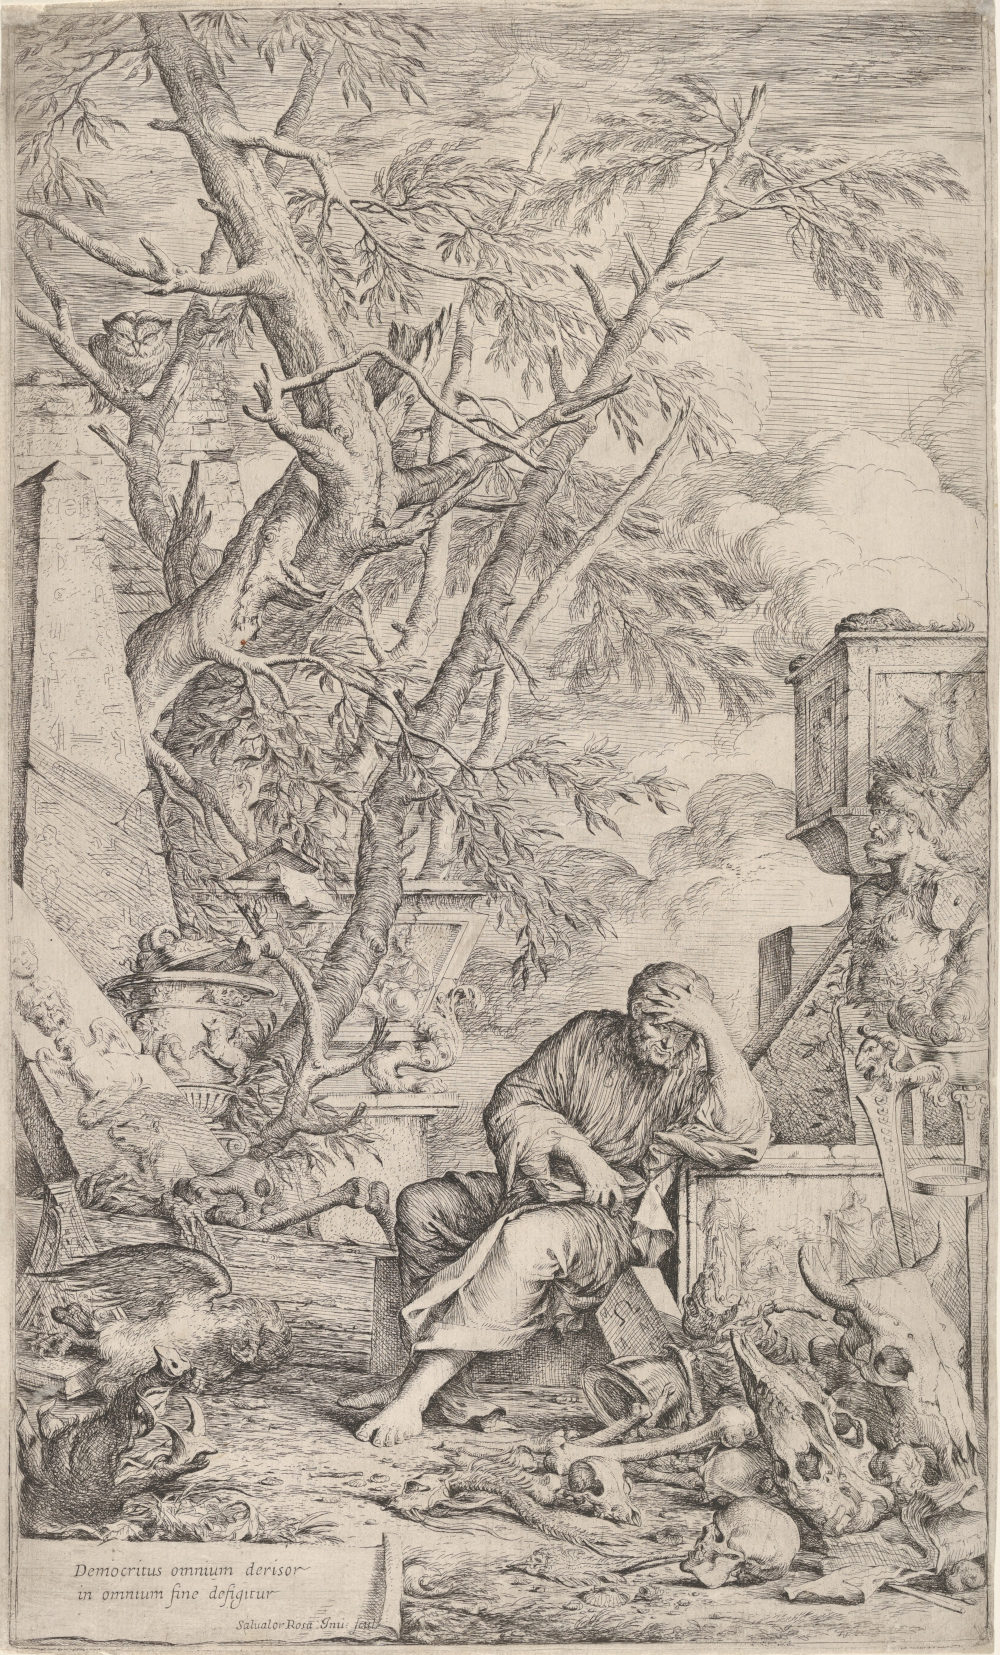
\includegraphics[keepaspectratio,width=0.9\textwidth]{Democritus-in-MeditationDP831915-small.jpg}
  \captionart{DemocritusinMeditation}
  \label{fig:democritusinmeditation}
\end{figure}
% Force float here
\clearpage{}
